\documentclass[nostrict]{szablonPG}

%-------------------- Dodatkowe pakiety ---------------------
\usepackage{listing}
\usepackage{dirtree}
\usepackage{comment}
\usepackage[x11names]{xcolor} % colorful text with the most amount of colors enabled (x11names)
\usepackage{graphicx}
\usepackage{pdflscape}
\usepackage{booktabs}
\usepackage{tabularx}
\usepackage[backend=biber,
            style=ieee,
            language=polish,
            giveninits=true,
            sorting=none,
            url=true,
            doi=false,
            isbn=false]{biblatex} % pakiet pozwalający na konfigurację bibliografi   
\addbibresource{refs.bib}
%------------------------------------------------------------
%------------------Definicja własnych komend-----------------
%------------------------------------------------------------
%------------------------------------------------------------
%			      Początek pracy dyplomowej  
%------------------------------------------------------------

\begin{document}

%------------------------------------------------------------
%  Dodanie strony tytułowej wygenerowanej z MojaPG oraz oświadczenia

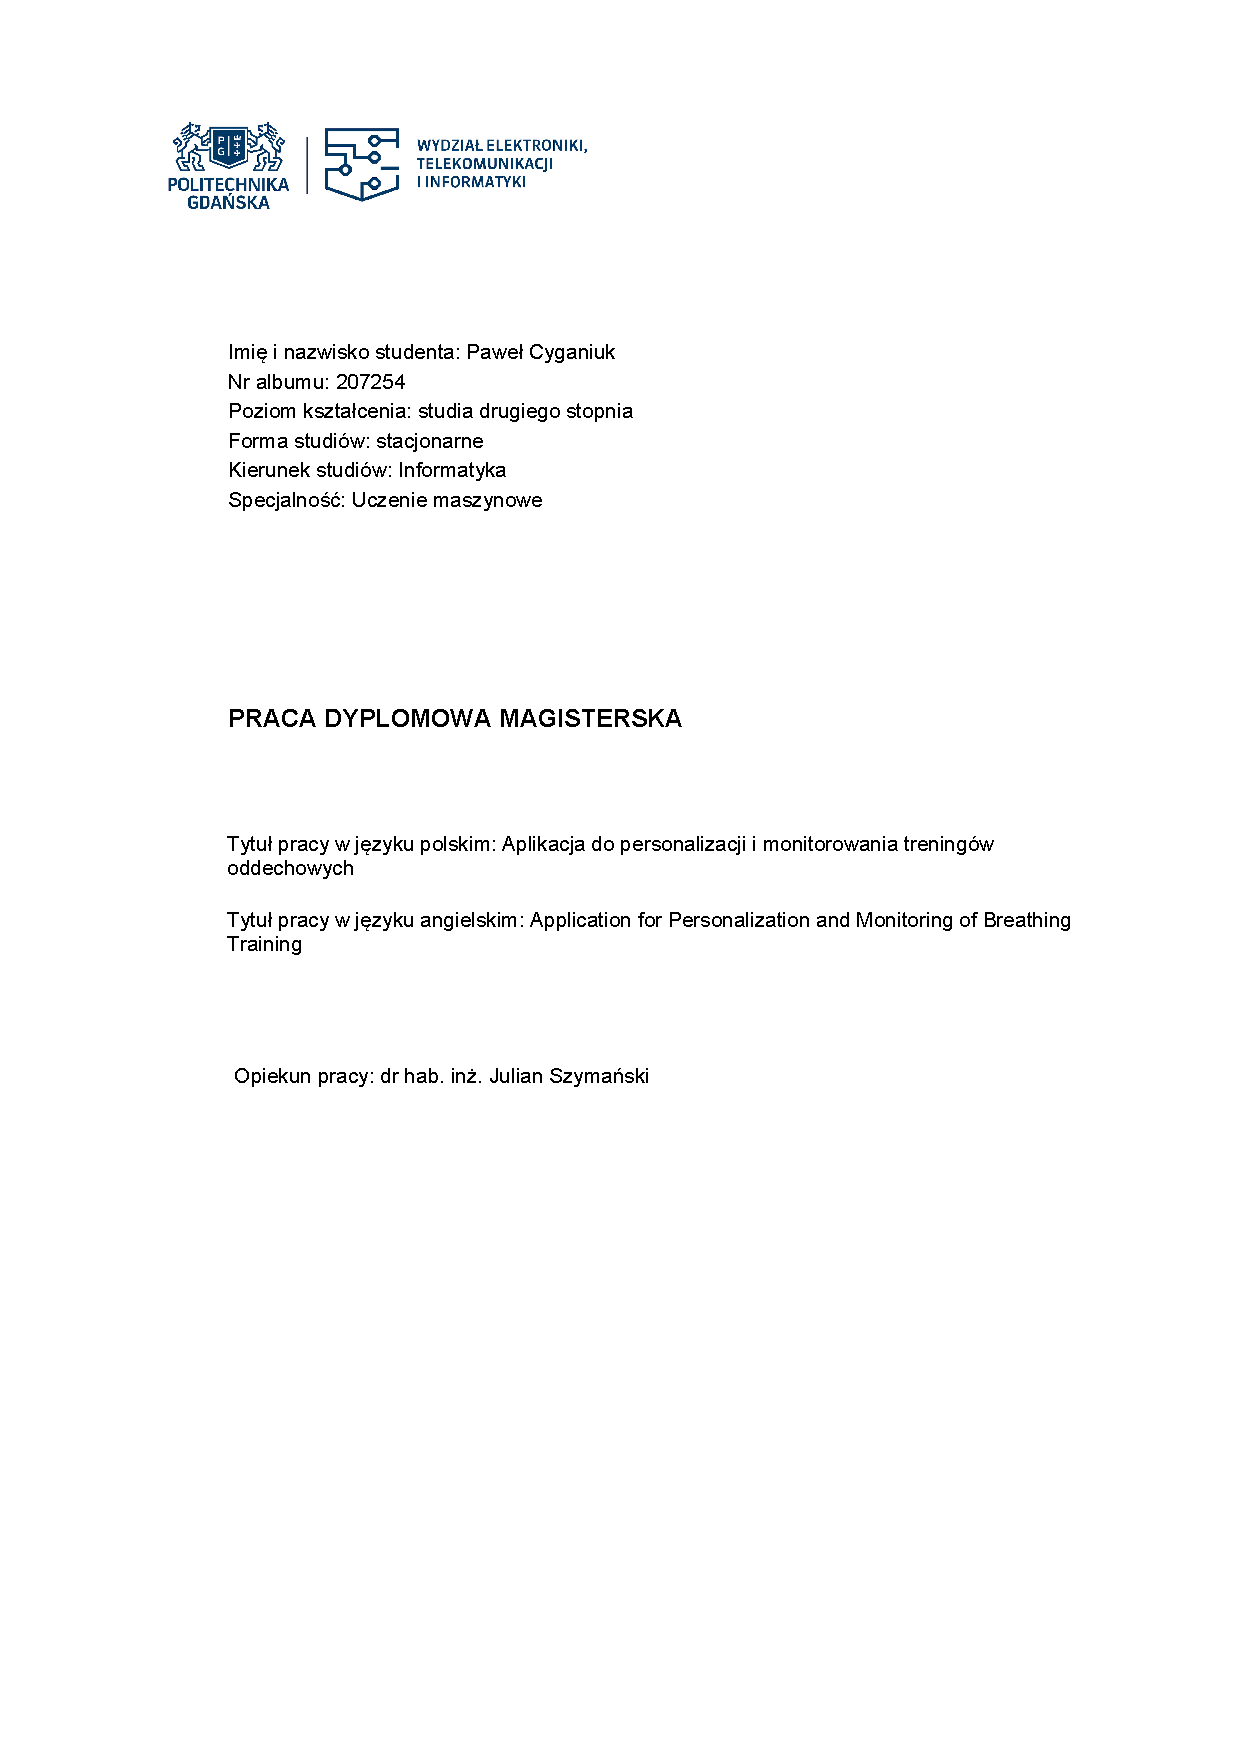
\includepdf[pages=-]{meta/StronaTytulowa_207254.pdf}
%\includepdf{meta/oswiadczenie.pdf}

%------------------------------------------------------------
%  Dodanie streszczenia i abstract
%  						

\chapter*{Streszczenie}

\indent W pracy przedstawiono rozwój aplikacji mobilnej ReSpire do spersonalizowanego treningu oddechowego oraz jej integrację z eksperymentalnym modelem wykrywania wydechu na podstawie dźwięku. Celem było wspomaganie ćwiczeń o konfigurowalnym przebiegu, a także zbadanie możliwości wykorzystania uczenia głębokiego do monitorowania cykli oddechowych za pomocą mikrofonu. Praca stanowi kontynuację istniejących projektów aplikacji i klasyfikacji oddechu, a przyjęte rozwiązania oparto na przeglądzie metod monitorowania oddechu, aplikacji mobilnych oraz sposobów wizualnego prowadzenia ćwiczeń.

Aplikację przygotowaną we Flutterze rozbudowano w zakresie konfiguracji i prowadzenia treningów oddechowych, dostosowując sposób jej obsługi do zróżnicowanych potrzeb użytkowników. Zmiany interfejsu uporządkowały prezentację ustawień, jak również zwiększyły możliwości personalizacji. Moduł detekcji wykorzystuje model CNN-Transformer rozwijany w PyTorch i wyeksportowany do formatu ONNX na potrzeby natywnej integracji z systemem Android. Udoskonalony model \textit{breathing classification v3} (BCV3) wytrenowano na rozszerzonym zbiorze danych, stosując regularyzację dropout oraz ważoną funkcję straty.

Modele BCV3 i BCV2 oceniono na wspólnym zbiorze testowym zawierającym 11~705 próbek dźwięku. Przy progu decyzyjnym 0,5 wersja ONNX modelu BCV3 osiągnęła dokładność 85,89\% i czułość wykrywania wydechu 94,52\%, wobec odpowiednio 84,95\% i 92,05\% dla BCV2. Wzrostowi czułości towarzyszyło zwiększenie liczby fałszywych detekcji. Testy na emulatorze Androida i urządzeniach fizycznych wskazały również na potrzebę dostosowywania progu decyzyjnego do konfiguracji rejestracji dźwięku.

Rezultatem pracy jest funkcjonalnie kompletna aplikacja do treningu oddechowego, wzbogacona o eksperymentalny moduł automatycznego zliczania cykli, stanowiący demonstrację wykonalności koncepcji (ang. \textit{proof of concept}). Dalsze prace mogą obejmować poprawę niezawodności detekcji, rozszerzenie rozpoznawania na wszystkie fazy oddechu oraz uzupełnienie natywnej integracji BCV3 w języku Swift dla systemu iOS, do którego warstwa aplikacyjna jest już przygotowana.

\vspace{0.5cm}
\noindent\textbf{Słowa kluczowe:} trening oddechowy, aplikacja mobilna, wykrywanie wydechu, uczenie głębokie, Flutter, ONNX\vspace{0.5cm}

\noindent \textbf{Dziedzina nauki i techniki, zgodnie z wymogami OECD:} nauki inżynieryjne i techniczne, nauka o komputerach i informatyce
\chapter*{Abstract}

\indent This thesis presents the development of ReSpire, a mobile application for personalised breathing training, and its integration with an experimental audio-based exhalation detection model. The aim was to support configurable breathing exercises and investigate the use of deep learning for monitoring breathing cycles through a microphone. The work builds on existing application and breath classification projects and draws on a review of breathing monitoring methods, mobile solutions, and visual guidance techniques.

The Flutter application was further developed to support the configuration and delivery of breathing training, with its interaction design adapted to diverse user needs. Interface changes improved the presentation of training settings and expanded personalisation options. The detection component uses a CNN-Transformer model developed in PyTorch and exported to ONNX for native integration on Android. The updated breathing classification v3 (BCV3) model was trained on an expanded dataset with dropout regularisation and a weighted loss function.

BCV3 and the baseline BCV2 were evaluated on the same test set of 11,705 audio samples. At a decision threshold of 0.5, the ONNX version of BCV3 achieved 85.89\% accuracy and 94.52\% exhalation recall, compared with 84.95\% and 92.05\% for BCV2. The improvement in recall was accompanied by an increase in false positive detections. Tests using an Android emulator and physical devices also indicated the need to adjust the decision threshold to the recording configuration.

The outcome is a functionally complete breathing training application enhanced with a proof-of-concept detection module for automatic cycle counting. Further work may improve detection reliability, extend recognition to all breathing phases, and complete the native Swift integration of BCV3 for iOS, for which the application layer is already prepared.

\vspace{0.5cm}
\noindent\textbf{Keywords:} breathing training, mobile application, exhalation detection, deep learning, Flutter, ONNX \vspace{0.5cm}


%------------------------------------------------------------
%   Lista komentarzy
% \listoftodos

%------------------------------------------------------------
%	Utworzenie spisu treści pracy dyplomowej
\tableofcontents

\chapter*{Wykaz ważniejszych oznaczeń i skrótów} % section* - ukrywa numerowanie oraz wyklucza ze spisu tresci
\addcontentsline{toc}{chapter}{Wykaz ważniejszych oznaczeń i skrótów}% % reczne dodanie do spisu tresci
\noindent
\textbf{UX} - (User Experience) doświadczenie użytkownika obejmujące jego odczucia i ocenę korzystania z aplikacji, w tym łatwość obsługi oraz możliwość realizacji zamierzonych celów. \newline
\textbf{UI} - (User Interface) interfejs użytkownika, czyli elementy umożliwiające komunikację z aplikacją, takie jak ekrany, przyciski, pola formularzy i komunikaty. \newline
\textbf{Spektrogram} - reprezentacja czasowo-częstotliwościowa sygnału przedstawiająca zmiany jego zawartości częstotliwościowej w czasie. Natężenie koloru obrazuje poziom poszczególnych składowych częstotliwościowych. \newline
\textbf{Macierz pomyłek} - (Confusion Matrix) tabela zestawiająca rzeczywiste klasy próbek z klasami przewidzianymi przez model. Pozwala określić liczbę poprawnych klasyfikacji oraz błędów dla poszczególnych klas. \newline
\textbf{CNN} - (Convolutional Neural Network) konwolucyjna sieć neuronowa wykorzystywana do analizy danych oraz ekstrakcji cech \cite{o2015introduction}. \newline
\textbf{RNN} - (Recurrent Neural Network) rekurencyjna sieć neuronowa przeznaczona do przetwarzania danych sekwencyjnych oraz analizy zależności czasowych \cite{grossberg2013recurrent}. \newline
\textbf{LSTM} - (Long Short-Term Memory) rodzaj rekurencyjnej sieci neuronowej umożliwiającej modelowanie zależności długoterminowych w danych sekwencyjnych \cite{hochreiter1997long}. \newline
\textbf{GRU} - (Gated Recurrent Unit) uproszczona architektura rekurencyjnej sieci neuronowej wykorzystująca mechanizmy bramkujące do efektywnego przetwarzania sekwencji danych \cite{cho2014learning}. \newline
\textbf{Transformer} - architektura sieci neuronowej oparta na mechanizmie self-attention, stosowana do przetwarzania danych sekwencyjnych oraz analizy zależności długoterminowych \cite{vaswani2017attention}. \newline
\textbf{Flutter} - otwartoźródłowy zestaw narzędzi programistycznych służący do tworzenia natywnych aplikacji mobilnych, webowych oraz desktopowych. \newline
\textbf{Dart} - obiektowy język programowania zoptymalizowany pod kątem tworzenia interfejsów użytkownika oraz aplikacji mobilnych, webowych i desktopowych. \newline
\textbf{iOS} - (iPhone Operating System) mobilny system operacyjny opracowany przez firmę Apple dla urządzeń mobilnych. \newline
\textbf{BEM} - (Breath Extraction Module) moduł ekstrakcji oddechu. \newline
\textbf{BPDM} - (Breathing Phases Detection Module) moduł detekcji faz oddechu. \newline
\textbf{ReLU} - (Rectified Linear Unit) jedna z najczęściej stosowanych funkcji nieliniowych w sieciach neuronowych. Przyjmuje wartość równą zero dla argumentów ujemnych oraz wartość równą argumentowi wejściowemu dla wartości nieujemnych. \newline
%------------------------------------------------------------
%	Dodanie rozdziałów pracy dyplomowej 

\chapter{Wprowadzenie}

\section{Wstęp}
Na przestrzeni ostatnich kilku lat można zaobserwować wzrost w zainteresowaniu różnego rodzaju technikami wspomagającymi zdrowie psychiczne jak i fizyczne \cite{ristovski2023importance}. Powodem tego jest między innymi stale rosnące tempo życia oraz coraz większe wymagania zawodowe i edukacyjne. Popularną metodą pomagającą radzeniu sobie z daną presją mogą być sesje ćwiczeń oddechowych przeprowadzane za pomocą filmów instruktażowych lub aplikacji mobilnych. 

W przypadku aplikacji mobilnych pożądane jest również możliwość personalizacji oraz monitorowanie treningu, aby użytkownik mógł dostosować odpowiednio poziom trudności czy otrzymać informację zwrotną jak dana sesja przebiegła.

\section{Cele pracy}
Celem pracy jest opracowanie narzędzia wspomagającego realizację treningów oddechowych w postaci aplikacji mobilnej, która umożliwi użytkownikowi definiowanie indywidualnych wzorców oddechowych oraz zapewni monitorowanie poszczególnych faz oddechu w czasie trwania sesji treningowej. 

W ramach badań przeprowadzona zostanie analiza istniejących metod monitorowania oddechu, zarówno wykorzystujących dedykowane czujniki, jak i rozwiązania oparte na powszechnie dostępnych urządzeniach mobilnych. Na podstawie przeprowadzonego przeglądu literatury oraz istniejących rozwiązań zostanie zaprojektowana i zaimplementowana aplikacja mobilna umożliwiająca realizację treningów oddechowych z możliwością personalizacji wzorców oddechowych. Dodatkowo do monitorowania wzorców oddechu skonstruowany zostanie model sztucznej inteligencji wykorzystujący uczenie głębokie. Opracowane rozwiązanie zostanie następnie poddane weryfikacji pod kątem poprawności działania oraz przydatności w kontekście wspomagania treningów oddechowych.

Wyniki pracy mogą przyczynić się do zwiększenia dostępności narzędzi wspierających praktykę ćwiczeń oddechowych, a także umożliwić ich łatwiejszą integrację z codziennym życiem użytkowników.
\chapter{Przegląd istniejących rozwiązań}

W niniejszym rozdziale przedstawione zostały istniejące rozwiązania oraz aplikacje dotyczące prowadzenia, wspomagania i analizowania treningów oddechowych. Oprócz tego zaprezentowano najpopularniejsze narzędzia oraz środowiska programistyczne używane do projektowania interfejsu, a także rozwijania aplikacji mobilnych. Omówione zostały również metody pozyskiwania i przetwarzania sygnału oddechowego za pomocą różnego rodzaju czujników. 

Przeanalizowano także współczesne metody wykorzystania sztucznej inteligencji w analizie sygnałów biomedycznych, ze szczególnym uwzględnieniem algorytmów uczenia głębokiego. Omówiono architektury oparte na splotowych sieciach neuronowych (CNN) \cite{o2015introduction}, wykorzystywanych do ekstrakcji cech z sygnałów czasowych i danych sensorycznych, rekurencyjnych sieciach neuronowych (RNN) \cite{grossberg2013recurrent}, w tym architekturach LSTM \cite{hochreiter1997long} oraz GRU \cite{cho2014learning}, umożliwiających modelowanie danych sekwencyjnych oraz analizę zmian sygnału w czasie, a także modele transformatorowe (Transformers) \cite{vaswani2017attention}, pozwalające na analizę zależności długoterminowych w sekwencjach danych. Przedstawiono możliwości zastosowania tych metod w kontekście detekcji wzorców oddechowych w czasie rzeczywistym jako informacji zwrotnej dla użytkownika.

\section{Rozwiązania wspierające treningi oddechowe}

Głównym kryterium podziału istniejących rozwiązań wpierających treningi oddechowe jest możliwość personalizacji oraz obecność funkcji analizy przebiegu sesji treningowej. W przypadku danych rozwiązań z perspektywy użytkownika bardzo ważnymi czynnikami w wyborze odpowiedniej metody prowadzenia własnego treningu jest dostępność czy wygoda użytkowania. 

Jedną z najbardziej dostępnych metod są filmy instruktażowe publikowane w portalach społecznościowych, jak na przykład „Wim Hof Method” \cite{wimhofbreathing}. Rozwiązania tego typu umożliwiają użytkownikowi wykonywanie ćwiczeń oddechowych bez konieczności korzystania ze specjalistycznego sprzętu lub oprogramowania. Pomimo licznych zalet rozwiązania te posiadają również istotne ograniczenia. Filmy instruktażowe nie oferują możliwości personalizacji treningu do indywidualnych potrzeb użytkownika ani monitorowania poprawności wykonywanych ćwiczeń.

W odpowiedzi na te ograniczenia rozwijane są aplikacje mobilne oraz systemy wykorzystujące czujniki i algorytmy sztucznej inteligencji do monitorowania sygnałów oddechowych. Rozwiązania te umożliwiają automatyczną analizę przebiegu treningu, wykrywanie wzorców oddechowych oraz dostosowywanie parametrów ćwiczeń do aktualnego stanu użytkownika. 

Spośród aplikacji mobilnych dostępnych jest na rynku sporo opcji. Oferują one jednak tylko element przeprowadzania treningu z nieznaczną personalizacją struktury treningu. 

\newpage

\subsection{Aplikacje komercyjne}
W danym segmencie pracy omówione zostaną aplikacje, które można znależć w sklepie z aplikacjami mobilnymi. Są to rozwiązania, które zostały pobrane przez setki tysięcy użytkowników na przestrzeni różnych platform. Zostały one przygotowane jako rozwiązanie gotowe do wypuszczenia na rynek.
\subsubsection{Wim Hof method}
Wśród aplikacji wspierających trening oddechowy wyróżnia się Wim Hof, która łączy ćwiczenia oddechowe z ekspozycją na zimno oraz elementami medytacji. Jej głównym celem jest umożliwienie użytkownikowi regularnego wykonywania treningów oddechowych w prosty i intuicyjny sposób.

Najważniejszą funkcjonalnością aplikacji są prowadzone sesje oddechowe. Użytkownik może wybierać spośród gotowych treningów oraz w ograniczonym zakresie dostosowywać ich parametry. Dostępne opcje obejmują m.in. zmianę liczby rund, tempa oddychania, liczby oddechów przed zatrzymaniem powietrza czy wybór podkładu muzycznego. W trakcie ćwiczeń aplikacja wyświetla animację pomagającą utrzymać odpowiedni rytm oddychania oraz informacje o aktualnej rundzie i liczbie wykonanych oddechów. Możliwe jest również wcześniejsze zakończenie sesji lub ręczne przejście do fazy zatrzymania oddechu.

Aplikacja oferuje także funkcje związane z monitorowaniem aktywności użytkownika. Dostępne są statystyki wykonanych treningów, kalendarz aktywności oraz system odznak motywujących do regularnych ćwiczeń. Dodatkowo użytkownik może udostępniać swoje wyniki i obserwować aktywność innych osób korzystających z aplikacji.

\begin{figure}[h]
    \centering

    \subfloat[Menu aplikacji]{
        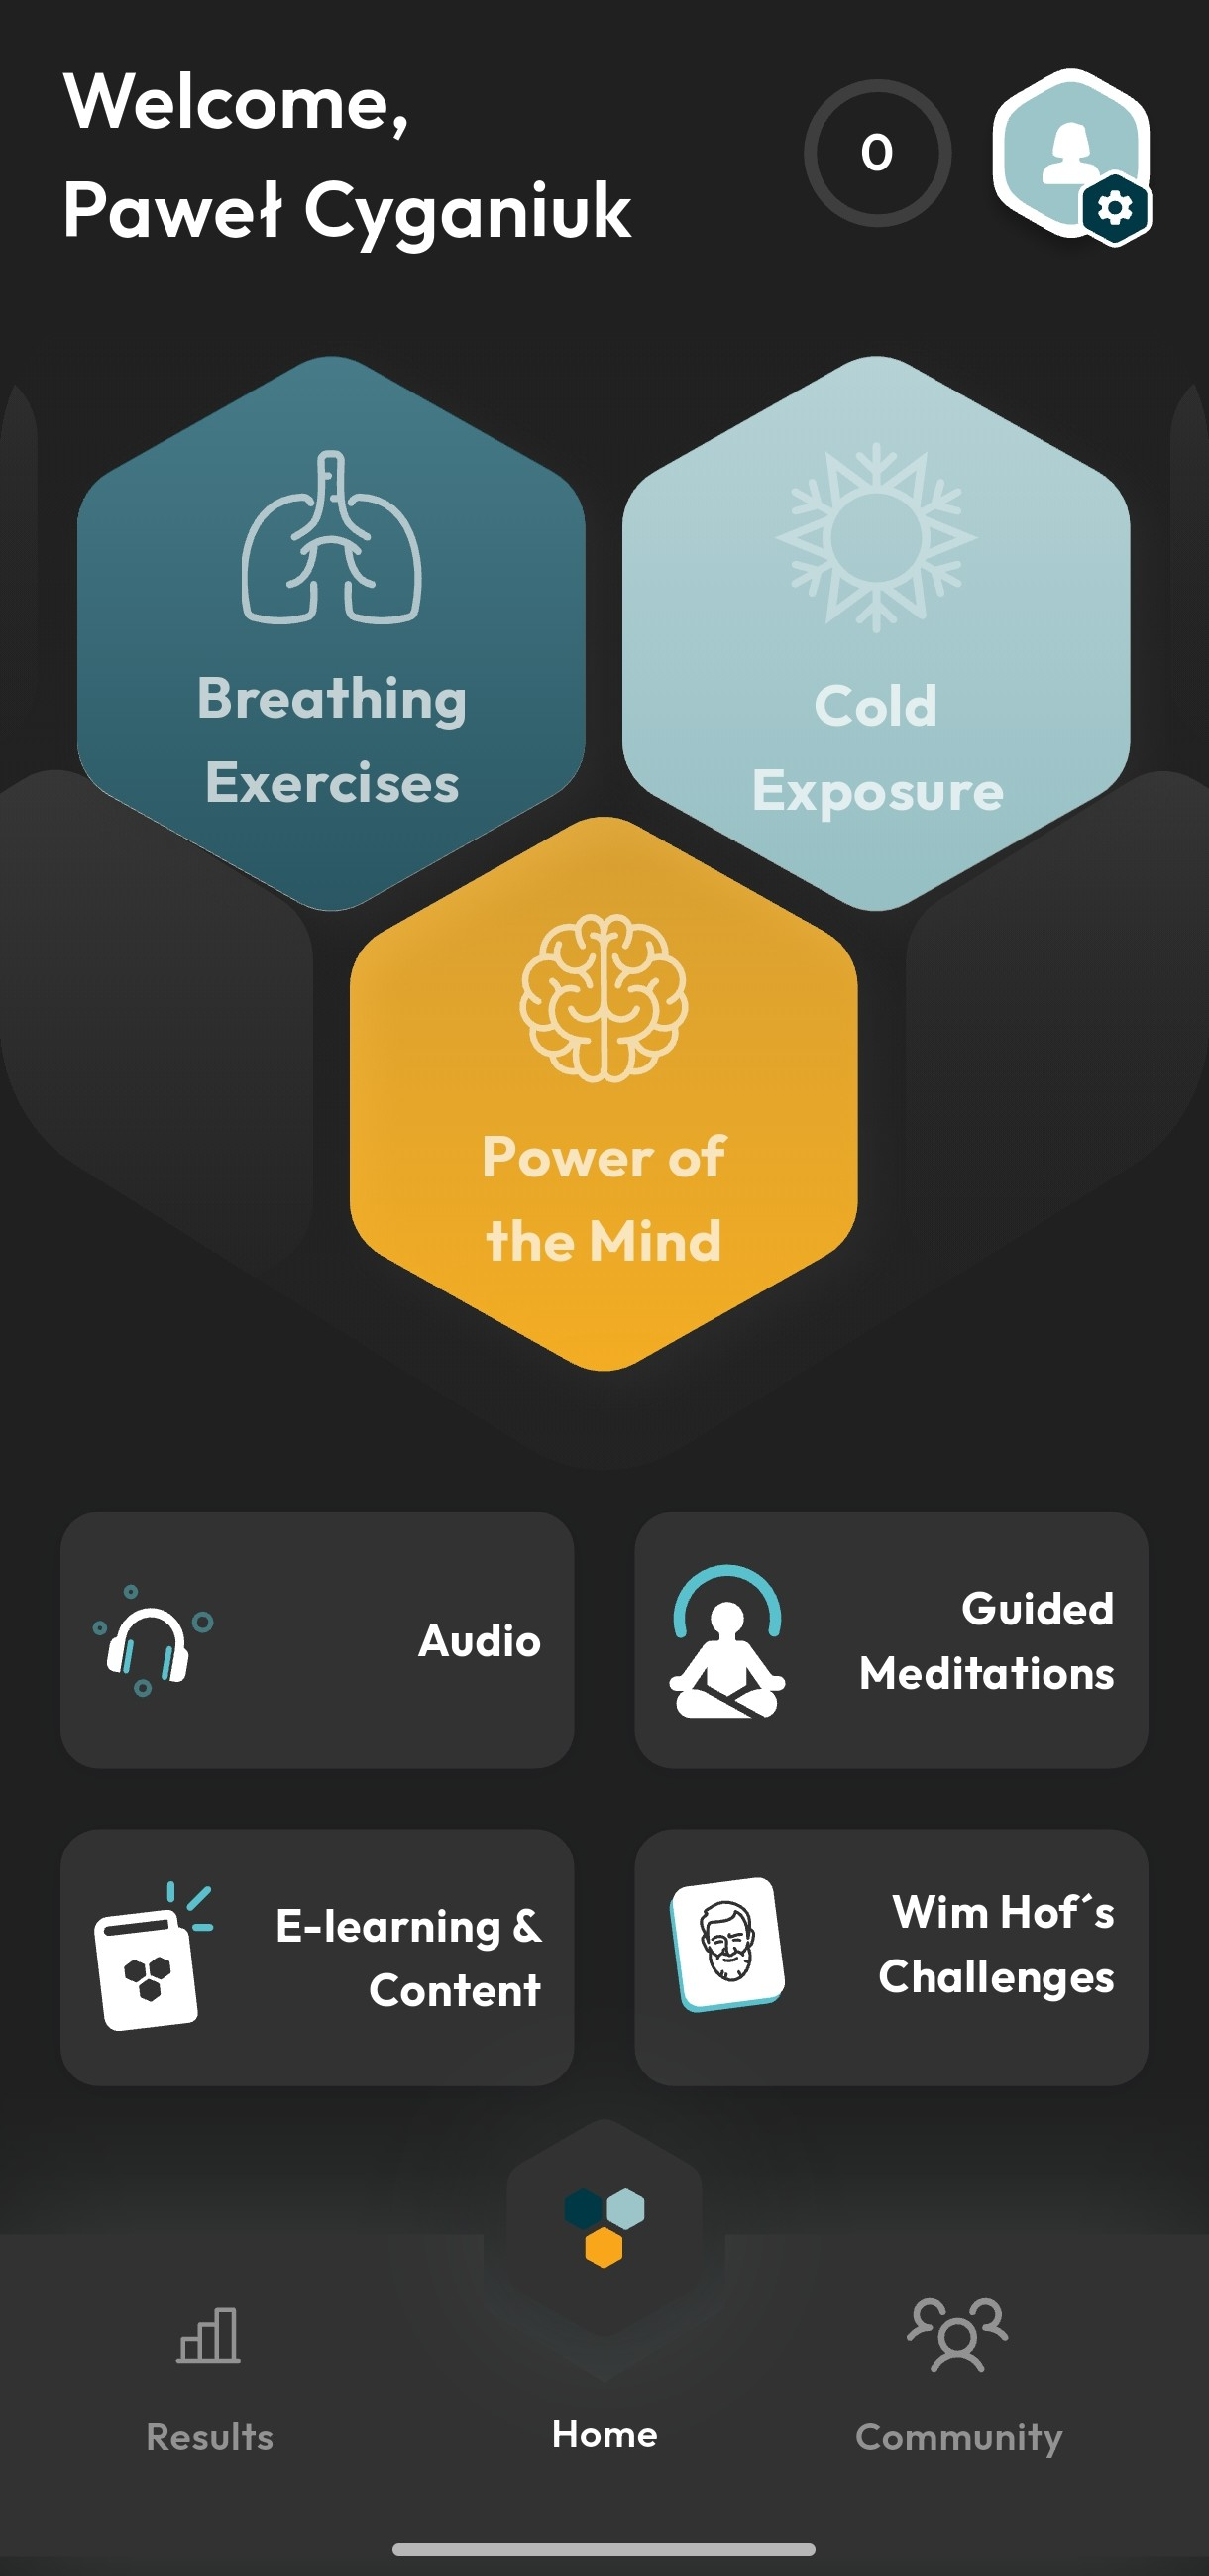
\includegraphics[width=0.27\textwidth,height=0.40\textheight,keepaspectratio]{obrazy/menu_wim.jpg}
    }
    \hfill
    \subfloat[Wizualizacja oddechu]{
        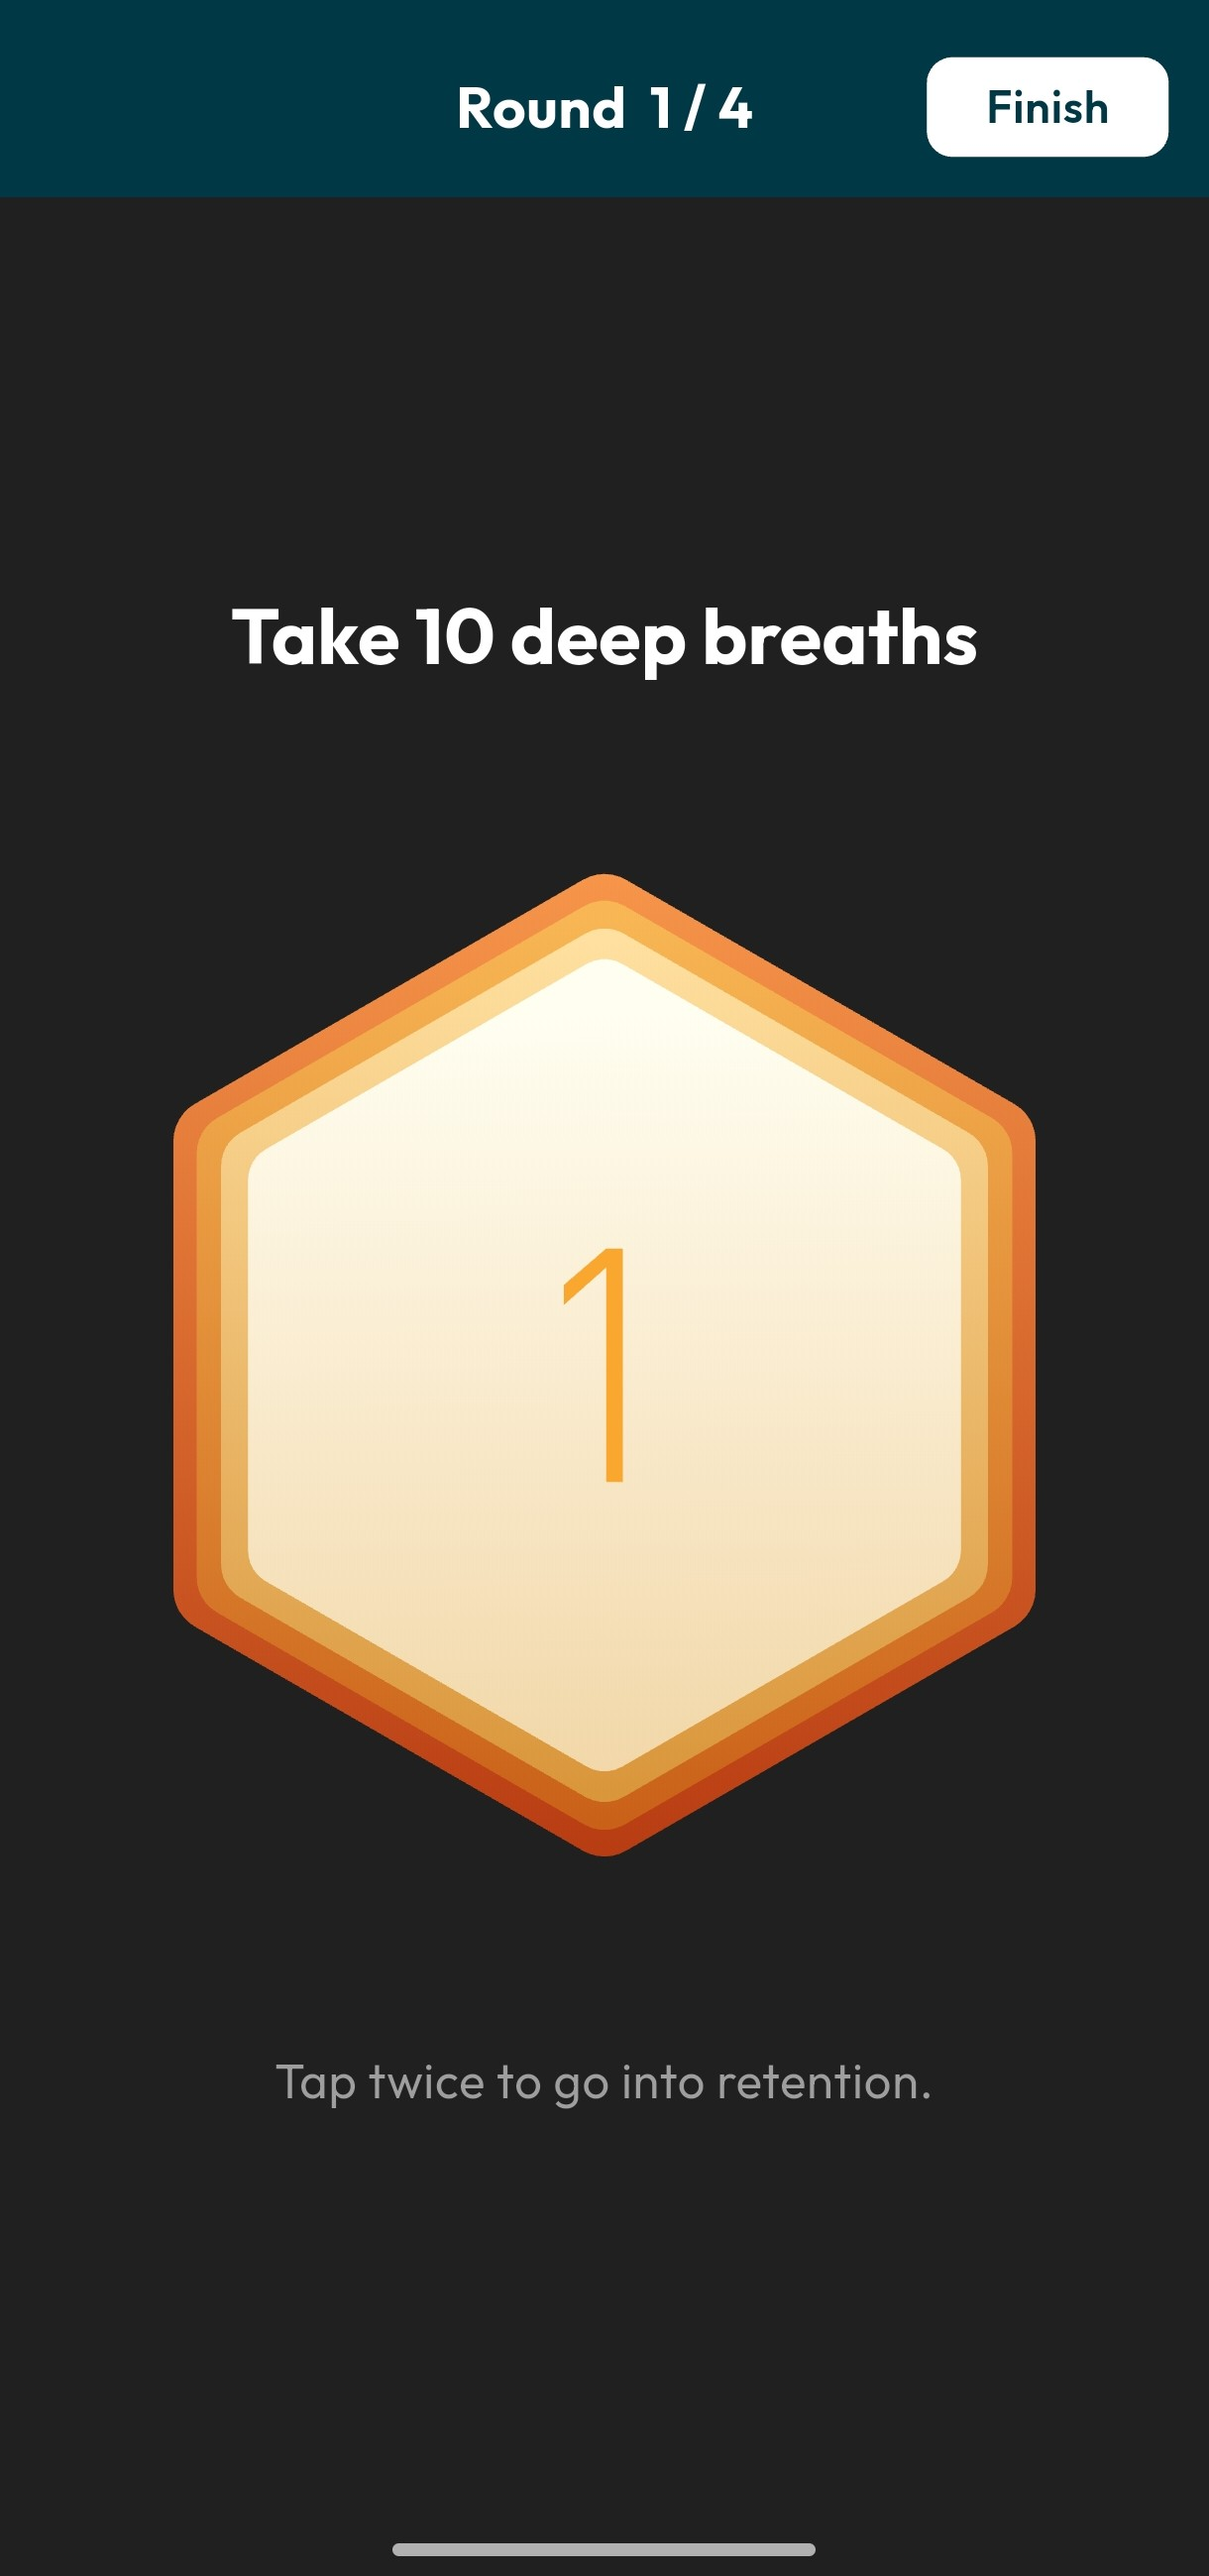
\includegraphics[width=0.27\textwidth,height=0.40\textheight,keepaspectratio]{obrazy/start_treningu_wim.jpg}
    }
    \hfill
    \subfloat[Wstrzymanie oddechu]{
        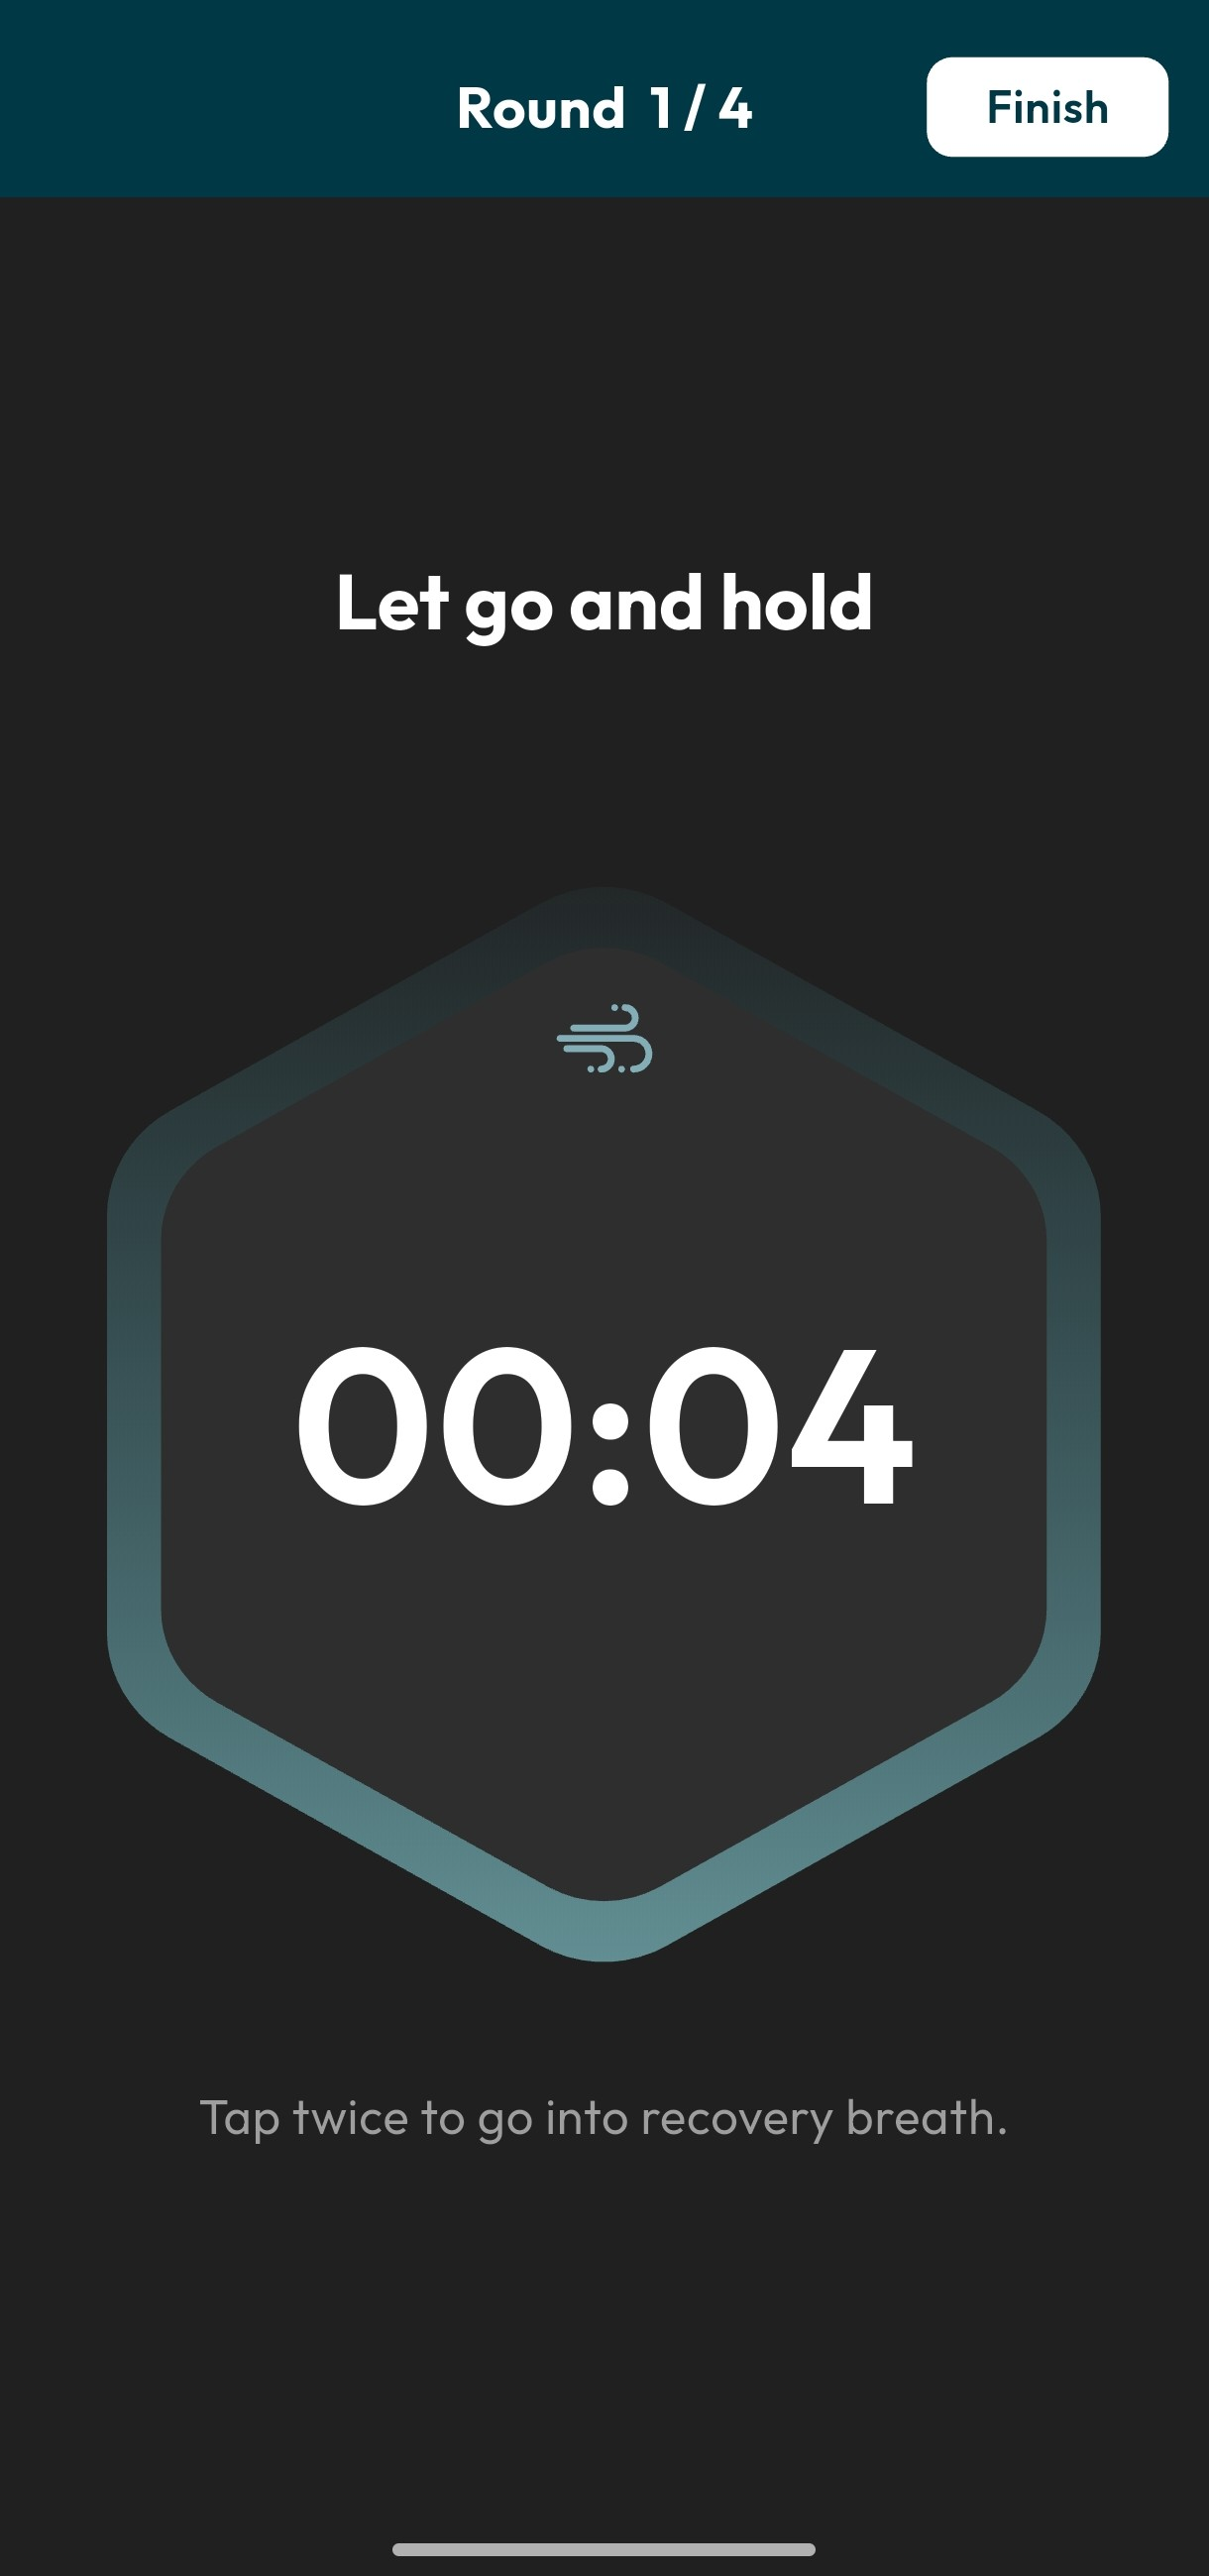
\includegraphics[width=0.27\textwidth,height=0.40\textheight,keepaspectratio]{obrazy/wstrzymanie_wim.jpg}
    }

    \caption{Zrzuty ekranu z aplikacji Wim Hof Method}
    \label{fig:wim_hof_method}
\end{figure}

Pomimo rozbudowanego systemu treningów aplikacja posiada istotne ograniczenia związane z personalizacją ćwiczeń. Użytkownik nie ma możliwości tworzenia w pełni własnych treningów ani swobodnego definiowania etapów sesji. Personalizacja ogranicza się jedynie do kilku podstawowych parametrów przygotowanych przez twórców aplikacji.
\subsubsection{Breathwrk}
Podobną aplikacją do wyżej wymienionej jest Breathwrk \cite{breathwrk2026}. W przeciwieństwie do Wim Hof Method, Breathwrk oferuje bardziej rozbudowaną bibliotekę treningów przeznaczonych do redukcji stresu, poprawy koncentracji, snu oraz zwiększania energii.

Istotnym elementem aplikacji są rozbudowane metody wizualizacji treningu. Podczas ćwiczeń użytkownik może korzystać z różnych animacji wyznaczających rytm oddechu, takich jak koło, linia czy animowane efekty immersyjne. Breathwrk kładzie większy nacisk na oprawę wizualną i dodatkowe bodźce, jak na przykład efekty świetlne, dźwięki tła czy wibracje telefonu synchronizowane z oddechem. Aplikacja umożliwia również korzystanie z instrukcji głosowych oraz ponowne uruchamianie treningu z wcześniej wybranymi ustawieniami.

Breathwrk oferuje także funkcje monitorowania aktywności użytkownika, takie jak statystyki treningów, poziomy rankingowe czy przypomnienia pomagające budować nawyk regularnych ćwiczeń. Podobnie jak w aplikacji Wim Hof Method, użytkownik może zapisywać ulubione treningi oraz śledzić swoje postępy.

\begin{figure}[h]
    \centering

    \subfloat[Menu aplikacji]{
        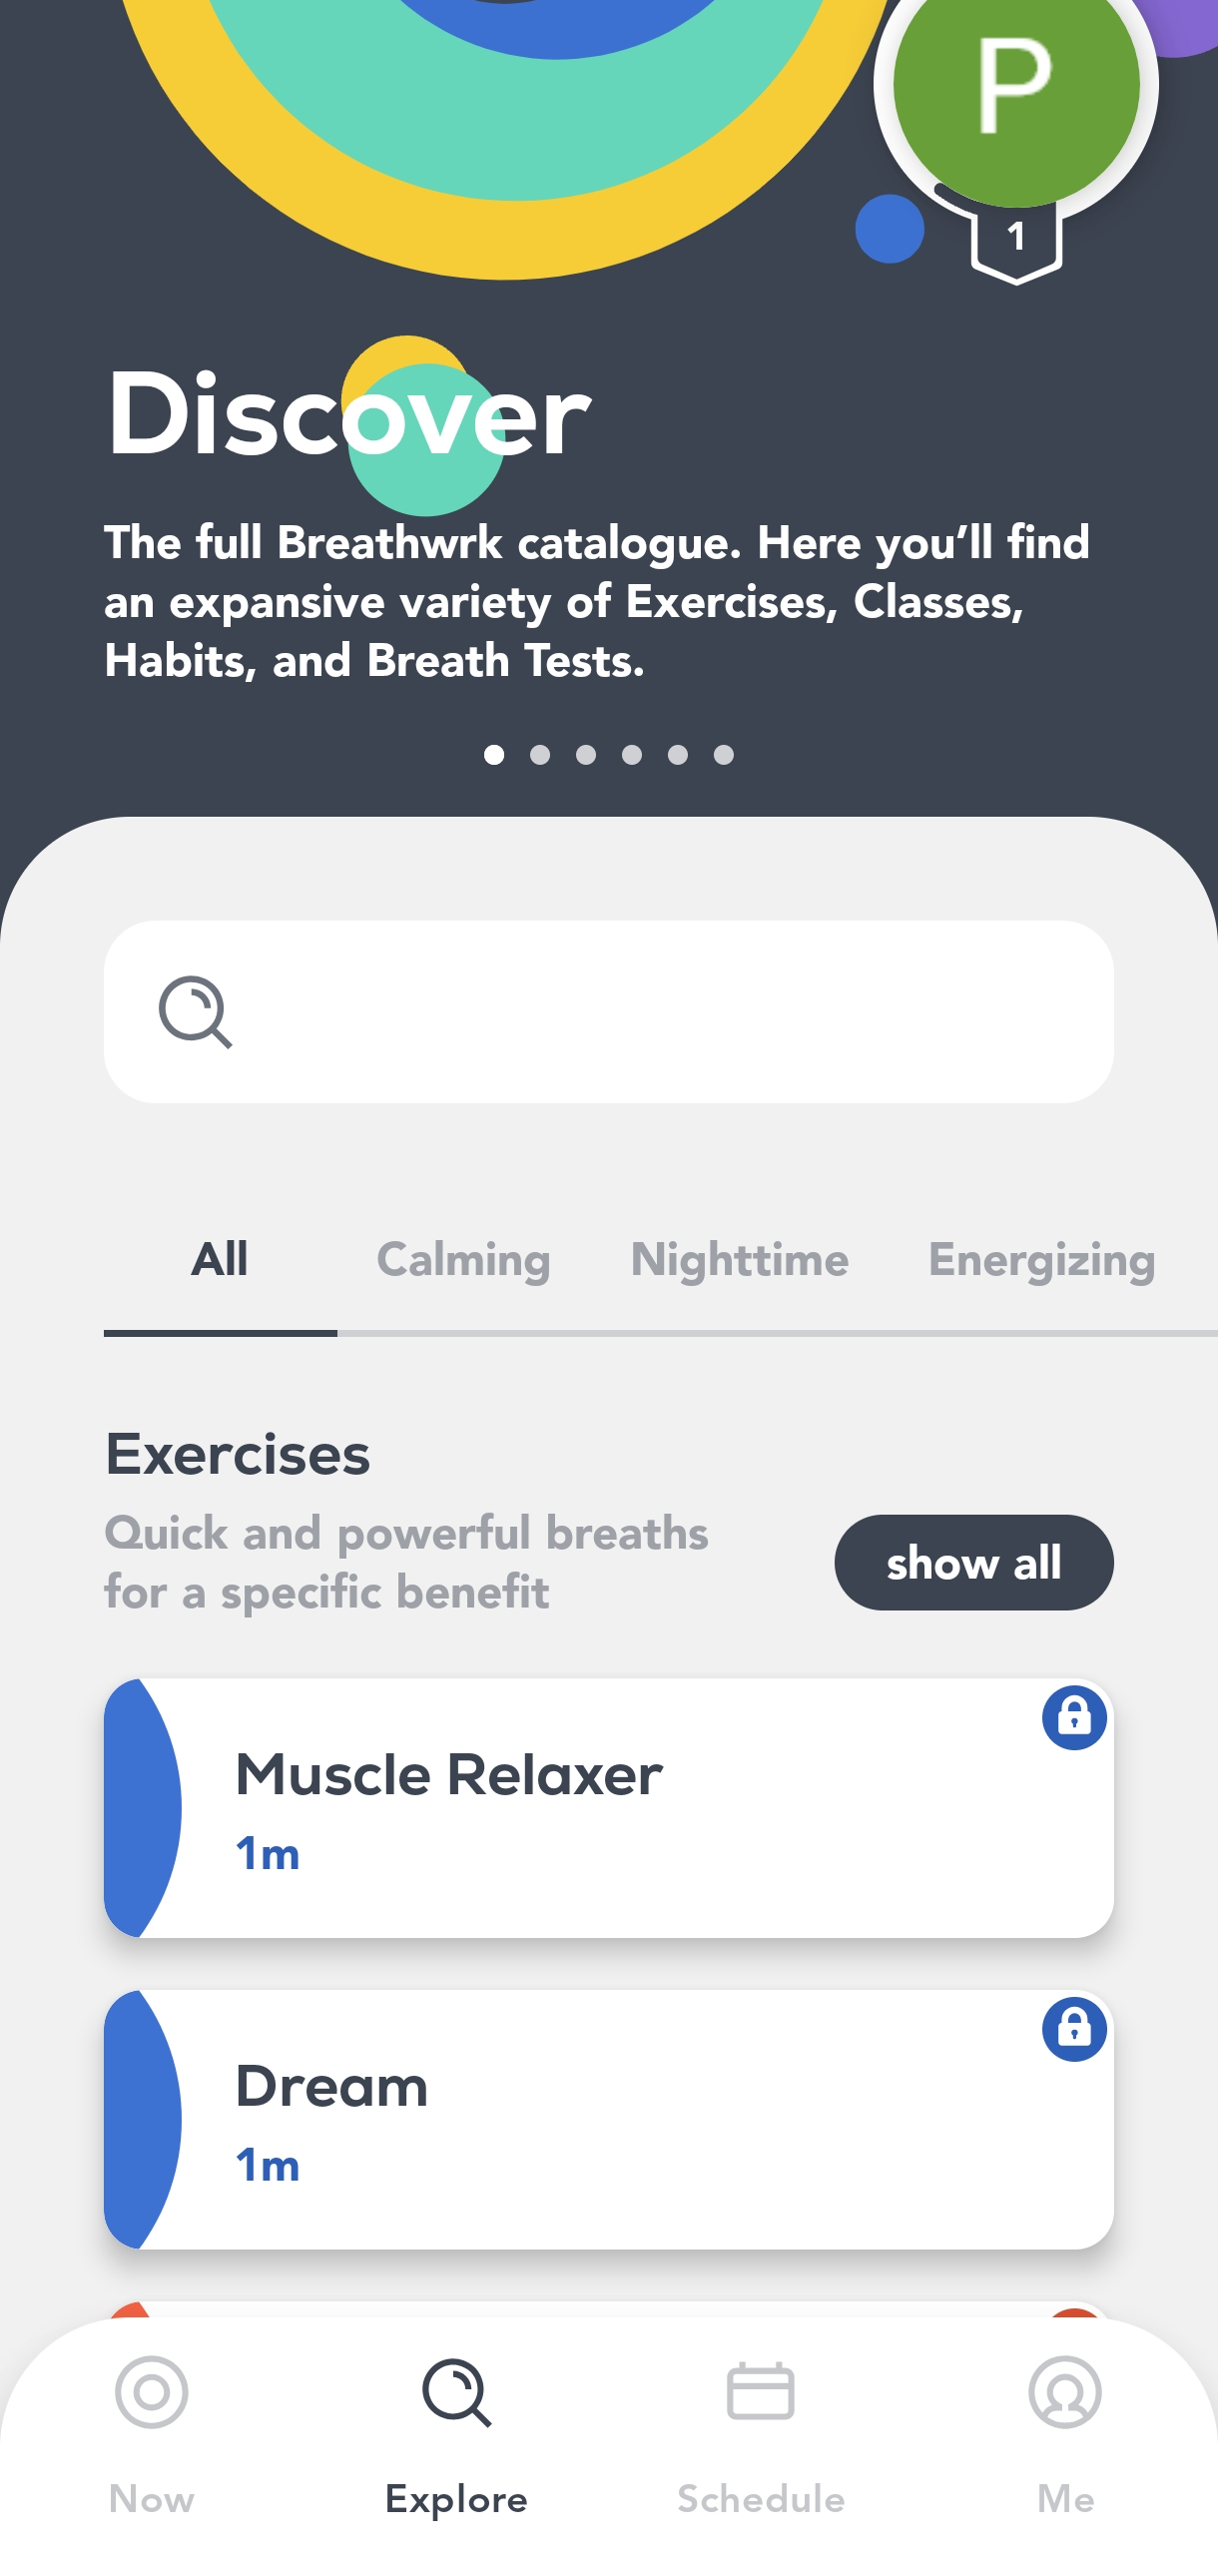
\includegraphics[width=0.27\textwidth,height=0.40\textheight,keepaspectratio]{obrazy/breathwrk_menu.jpg}
    }
    \hfill
    \subfloat[Standardowa wizualizacja oddechu]{
        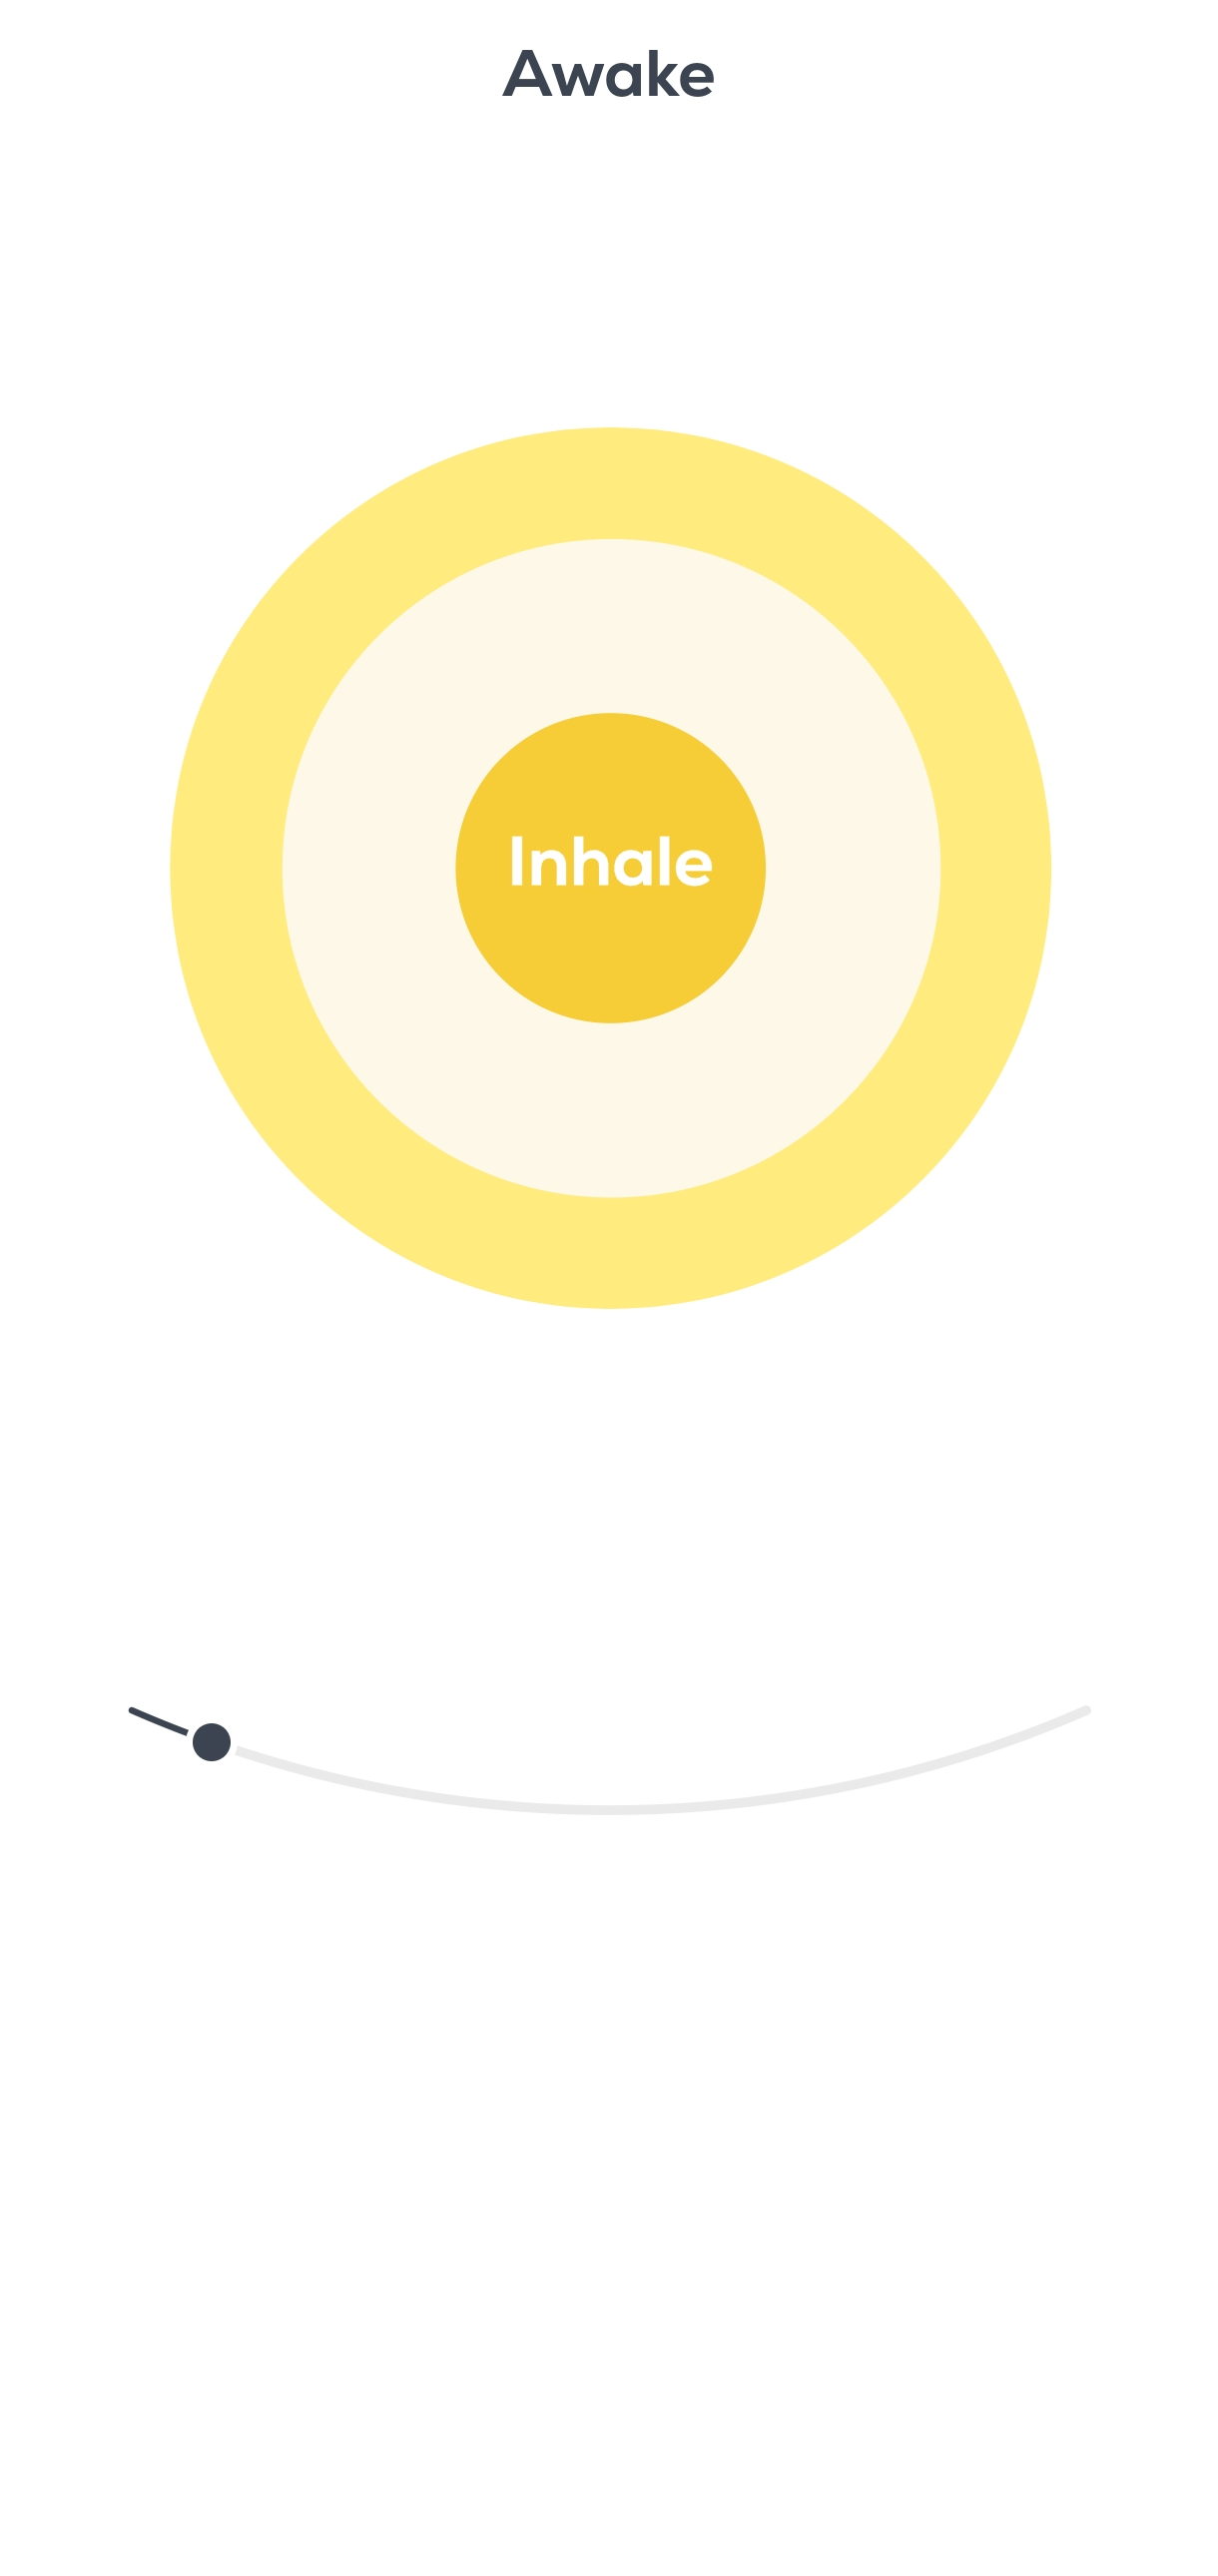
\includegraphics[width=0.27\textwidth,height=0.40\textheight,keepaspectratio]{obrazy/breathwrk_training_normal.jpg}
    }
    \hfill
    \subfloat[Immersywna wizualizacja oddechu]{
        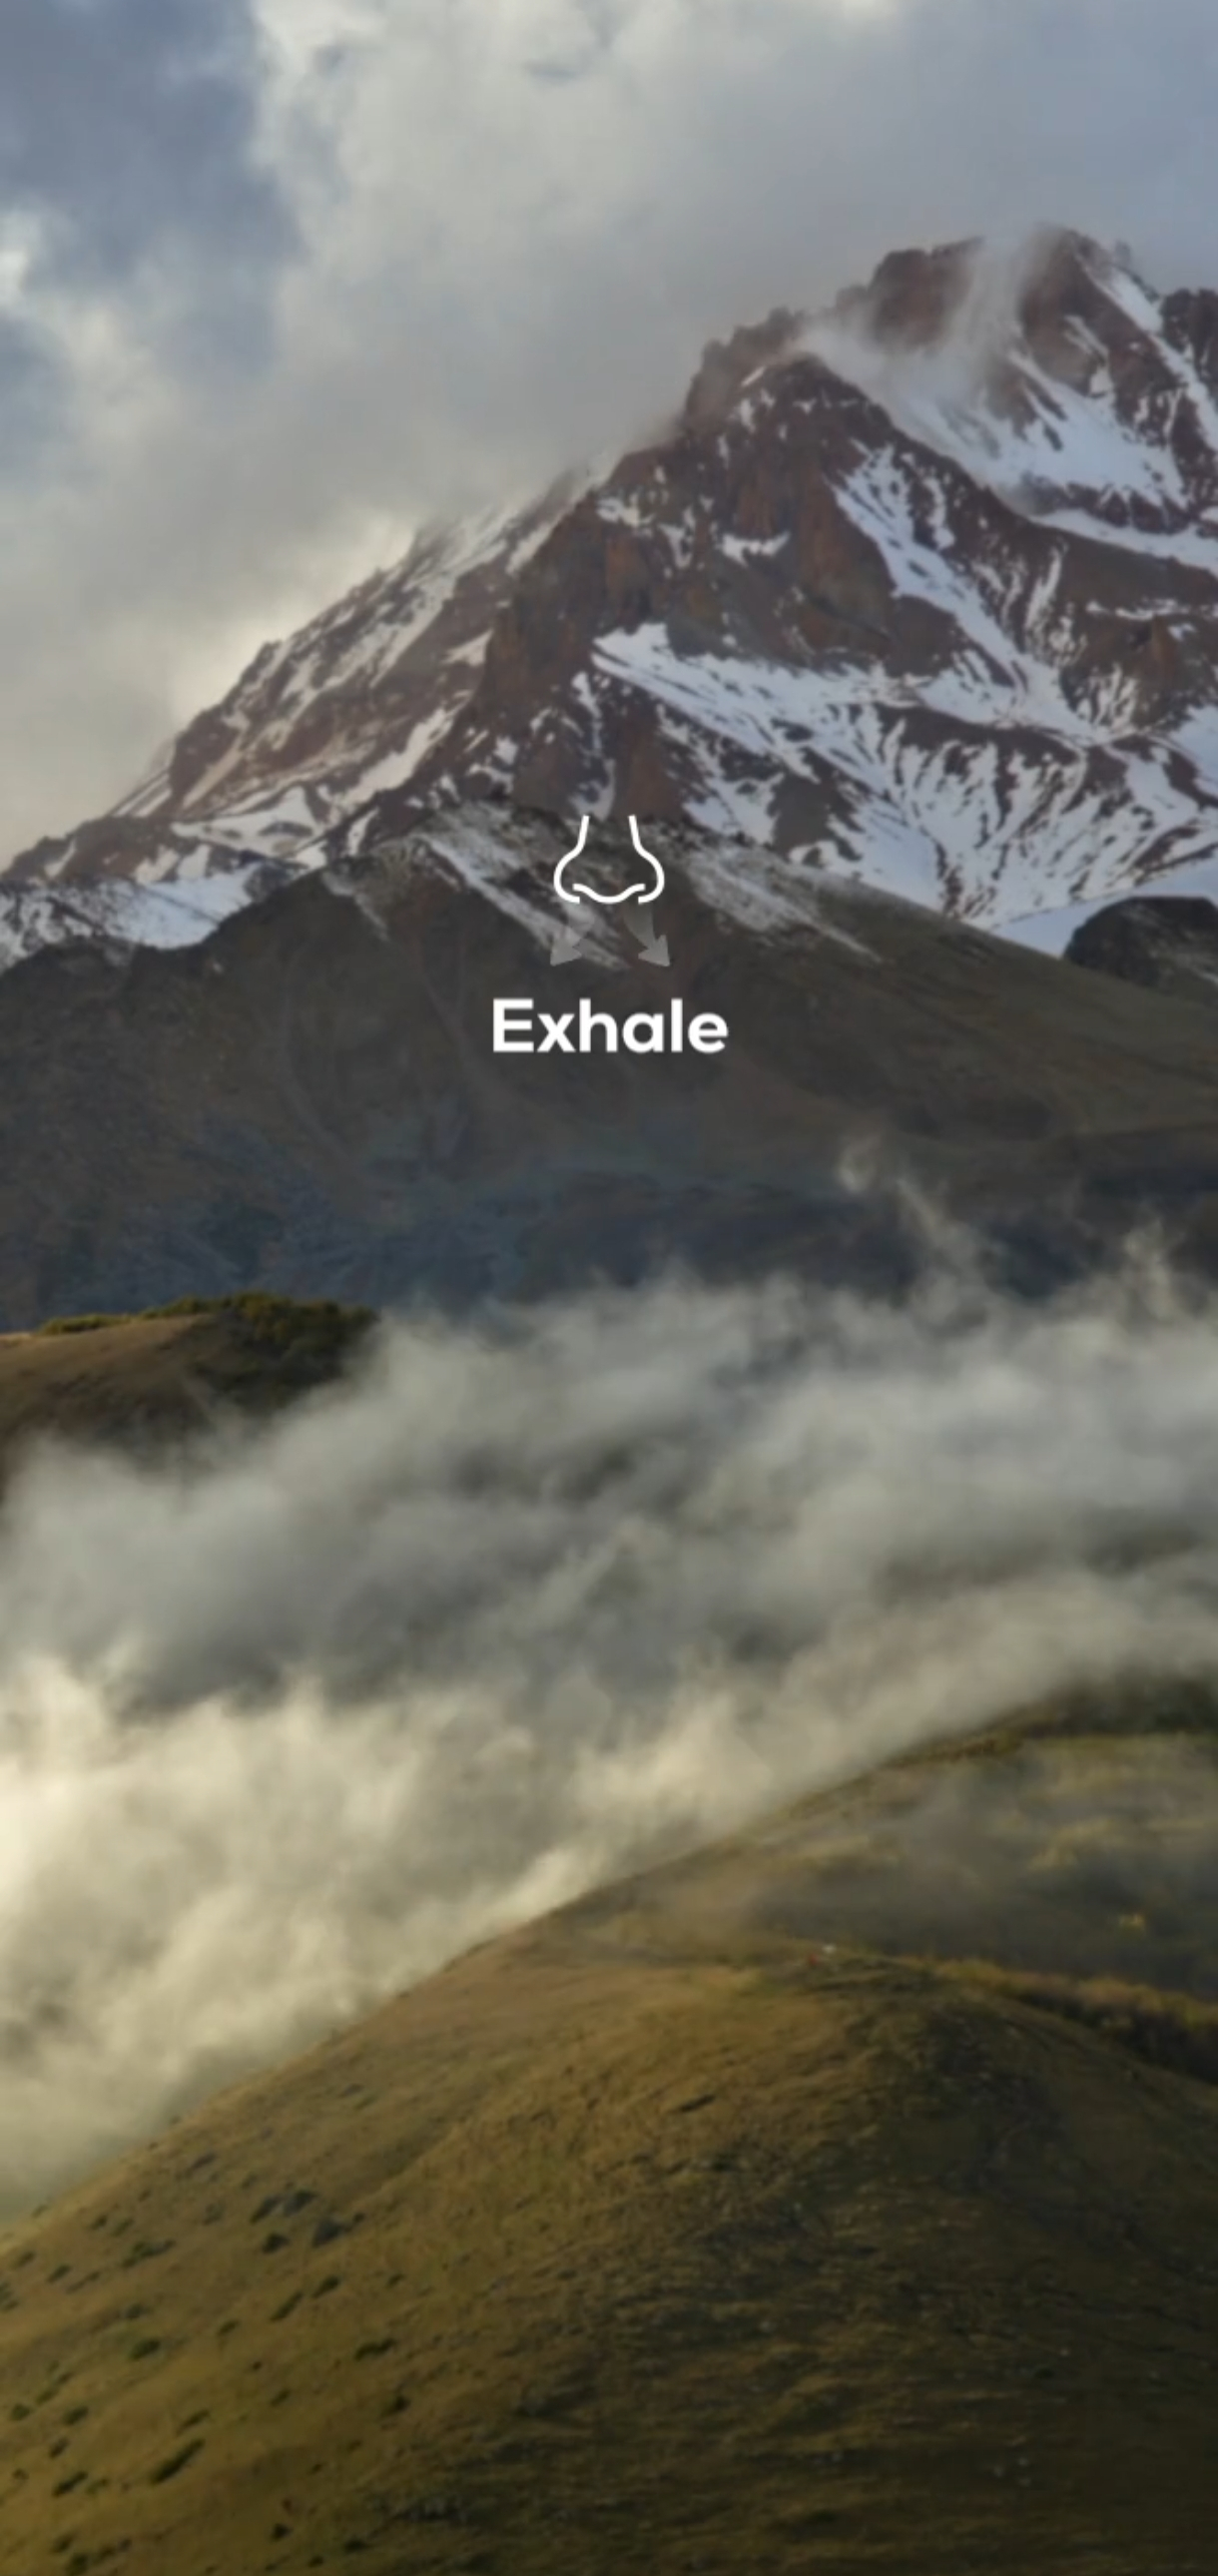
\includegraphics[width=0.27\textwidth,height=0.40\textheight,keepaspectratio]{obrazy/breathwrk_training_sky.jpg}
    }

    \caption{Zrzuty ekranu z aplikacji Breathwrk}
    \label{fig:breathwrk}
\end{figure}
Pomimo większego nacisku na warstwę wizualną i różnorodność gotowych treningów, aplikacja nadal posiada ograniczenia związane z personalizacją. Użytkownik nie może tworzyć własnych sesji oddechowych ani swobodnie definiować długości poszczególnych etapów ćwiczenia. Możliwa jest jedynie częściowa modyfikacja parametrów treningu, a część funkcji dostępna jest wyłącznie w wersji Premium.


\subsection{Aplikacje wspierające monitorowanie oddechu}
\subsubsection{Breeze}
Istotnym przełomem technologicznym w kontekście monitorowania oddechu jest rozwiązanie o nazwie Breeze \cite{10.1145/3369835}. Autorzy opracowali aplikację mobilną, która całkowicie eliminuje konieczność stosowania zewnętrznych urządzeń sensorycznych. Aplikacja wykorzystuje wyłącznie wbudowany w smartfon mikrofon do ciągłej detekcji faz oddechu użytkownika w czasie bliskim rzeczywistemu. Umożliwia ona realizację przetestowanego klinicznie wzorca oddechowego "4-2-4", składającego się z czterech sekund wdechu, dwóch sekund wydechu oraz czterech sekund pauzy, celując w indukcję oddechu z częstotliwością sześciu pełnych cykli na minutę. Aby zrealizować takie rozwiązanie w praktyce, konieczne było przezwyciężenie trudności związanych z niskim stosunkiem sygnału do szumu (SNR), zwłaszcza ze względu na niemal niesłyszalny dla mikrofonu dźwięk wdechu naturalnego.

Kluczowym elementem wkładu badawczego autorów pracy jest stworzenie bardzo dokładnego potoku przetwarzania sygnału akustycznego. Odebrany przez mikrofon dźwięk jest analizowany w jedno-sekundowych oknach. Na początku sygnał poddawany jest wstępnemu przetwarzaniu z użyciem filtrów pasmowo-przepustowych, a następnie, przy pomocy przesuwnych okien czasowych o długości 44 ms i nakładaniu 75\%, wyodrębniane są cechy częstotliwościowe, w tym charakterystyki w skali logMel oraz współczynniki melcepstralne (MFCC). Tak przygotowane dane wejściowe przekazywane są do dwuetapowego modelu rozpoznawania opartego o architekturę głębokich sieci neuronowych.  

\begin{figure}[h]
    \centering
    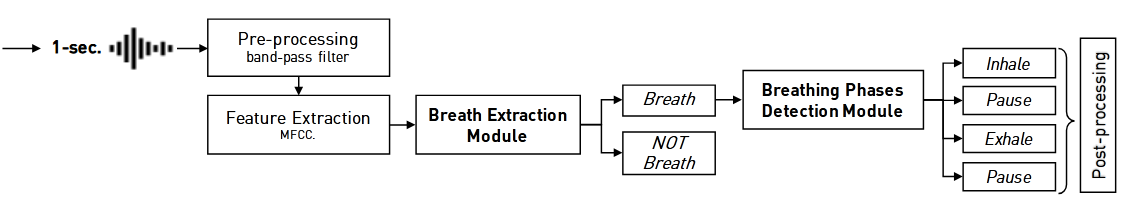
\includegraphics[width=1.0\linewidth]{obrazy/breeze_pipeline.png}
    \caption{Pipeline obróbki sygnału dźwiękowego aplikacji Breeze}
    \label{fig:breeze_pipeline}
\end{figure}

Proces przetwarzania sygnału dźwiękowego pozyskiwanego z mikrofonu urządzenia mobilnego został przedstawiony na Rysunku \ref{fig:breeze_pipeline}. Pierwszą warstwę detekcji stanowi Moduł Ekstrakcji Oddechu (BEM). Pełni on rolę zaawansowanej bramki kalibracyjnej, oddzielającej sygnał właściwy od dźwięków tła takich jak mowa, kaszel czy śmiech. Moduł BEM oparto o jednowarstwową splotową sieć neuronową (CNN) stosującą dziesięć filtrów, funkcję aktywacji ReLU oraz końcową klasyfikację klas za pomocą warstwy w pełni połączonej (FC) z funkcją softmax. Wyizolowane dzięki BEM ramki dźwiękowe zawierające poprawny sygnał oddechowy trafiają z kolei do Modułu Detekcji Faz (BPDM). Biorąc pod uwagę podobieństwo właściwości akustycznych wdechu i wydechu, autorzy odeszli od analizy niezależnych klatek dźwięku na rzecz analizy wzorców w czasie. Zastosowano tu dwukierunkową sieć z pamięcią długoterminową i krótko-terminową (BiLSTM), wzbogaconą o mechanizm uwagi. Mechanizm uwagi pozwala modelowi dynamicznie alokować "skupienie"~na tych fragmentach długiej sekwencji dźwiękowej, które niosą ze sobą największą wartość informacyjną w określeniu bieżącej fazy. Ostateczny wynik optymalizowany jest poprzez algorytm post-processingu w celu uniknięcia migotania fałszywych odczytów i zapewnienia płynnego interfejsu.  

Dla wytrenowania powyższych algorytmów konieczne było skompletowanie wysoce zróżnicowanego zbioru danych. Autorzy przeprowadzili sesję rejestracji danych z udziałem 43 uczestników, tworząc bazę ponad 2,76 miliona zdarzeń oddechowych. Aby system był uniwersalny i niezależny od specyfikacji sprzętowej konkretnego telefonu, próbki zbierano jednocześnie na czterech różnych urządzeniach mobilnych oraz dodatkowo na referencyjnym mikrofonie studyjnym. Dodatkowo użyty został bezprzewodowy pas mierzący ekspansję klatki piersiowej, pełniący funkcję fizjologicznego punktu odniesienia. Dane poddano półautomatycznemu etykietowaniu, gdzie oprócz informacji z sensora na ciele korzystano m.in. z filtru Savitzky'ego-Golay'a \cite{5888646} oraz algorytmu dekodowania Viterbiego do identyfikacji poszczególnych faz cyklu.  

% TU SKONCZYŁEM NA RAZIE

\begin{figure}[h]
    \centering
    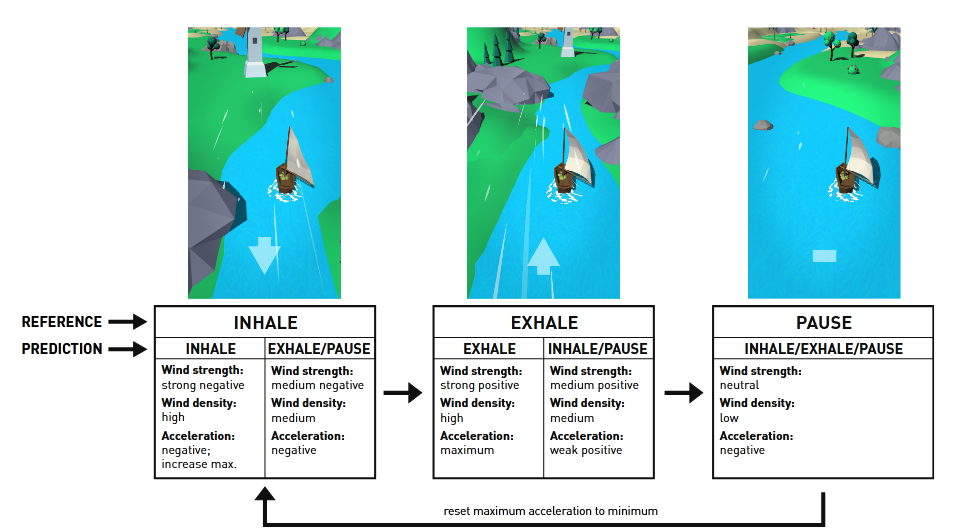
\includegraphics[width=0.80\linewidth]{obrazy/breeze_screen.png}
    \caption{Sposób działania aplikacji Breeze}
    \label{fig:breeze_workflow}
\end{figure}

Oprócz samego przetwarzania sygnałów, system Breeze kładzie również nacisk na element grywalizacji, który ma bezpośrednie przełożenie na monitorowanie treningu oraz satysfakcję i motywację końcowego użytkownika. Wygenerowane wyniki faz oddechu uruchamiają dynamiczny, wizualny moduł zbudowany w środowisku silnika Unity. Ćwiczenia przybierają formę sterowania żaglówką za pomocą wykrywania faz oddechu. Gdy system wykryje, że użytkownik poprawnie realizuje nałożony profil "4-2-4"~nagradza on gracza odpowiednim poruszeniem łódki i zachowaniem środowiska. Wdech napędza oraz generuje cząsteczki wiatru, podczas gdy wydech wydyma żagiel i gwarantuje płynne przyśpieszenie obiektu. Tego typu biofeedback w środowisku naturalnym stanowi ważną wartość empiryczną dla odbiorców, a także zwiększa ich zaangażowanie. Oprócz tego widać również, że sama kolorystyka aplikacji została dopasowana tak aby działała kojąco i~uspokajająco na użytkownika. 

Jeśli chodzi o wyniki samego modelu zaproponowanego przez autorów to ewaluacja wydajności technologicznej oraz testy kliniczne potwierdzają ogromny potencjał opisanego systemu. Moduł ekstrakcji (BEM) wytrenowany we wspartym głębokim uczeniem środowisku osiągnął precyzję AUC wynoszącą 0,92. Detektor poszczególnych faz oddechowych (BPDM) uzyskał wysoką w warunkach rzeczywistych skuteczność klasyfikacji na poziomie 75,5\%. Co więcej, złożony potok aplikacji wymaga zaledwie od 2,65 mln do ok. 10 mln operacji zmiennoprzecinkowych i w teście na telefonie z procesorem Snapdragon 845 wykazał opóźnienia detekcji na bardzo niskim poziomie 119 milisekund, umożliwiając płynne wyświetlanie animacji w 30 klatkach na sekundę przy jednoczesnej analizie dźwięku bez nadmiernego obciążania procesora.  

Dodatkowo, badanie pilotażowe na grupie 16 ochotników dowiodło mierzalnych, medycznych zalet działania omawianego rozwiązania. Korzystanie ze smartfona z aplikacją Breeze doprowadziło do znacznego obniżenia częstotliwości oddechów użytkowników (z poziomu ok. 12 oddechów spoczynkowo do pożądanych ok. 6 cykli na minutę). Rejestrowane równolegle wartości elektrokardiogramu (EKG) ujawniły statystycznie istotny i znaczny wzrost parametru wariancji tętna (HF-HRV) względem stanu bazowego. Były to wyniki wyższe, a także lepsze niż dla grupy kontrolnej, która podążała za prostą animacją na ekranie niezawierającą aktywnego biofeedbacku. Z~perspektywy ewaluacji UX, interaktywna koncepcja przewyższyła standardowe metody niemal we wszystkich wymiarach, takich jak:
\begin{itemize}
    \item podwyższone uczucie immersji,
    \item dobrze odczuwalna responsywność aplikacji,
    \item pozytywne doświadczenie z używania aplikacji.
\end{itemize} 

Podsumowując, choć system Breeze stanowi interesujący przykład wykorzystania uczenia maszynowego w monitorowaniu parametrów życiowych, jego praktyczna użyteczność w warunkach rzeczywistych budzi pewne zastrzeżenia. Zaproponowana architektura oparta na sieciach splotowych i rekurencyjnych oraz pozyskiwaniu sygnału z mikrofonu samego urządzenia wykazuje zadowalającą skuteczność przede wszystkim w kontrolowanym środowisku, co może znacząco ograniczać jej niezawodność w obecności dynamicznego szumu otoczenia czy różnych specyfikacji mikrofonów w tańszych urządzeniach mobilnych.

Kluczowym problemem z perspektywy dalszego rozwoju tej technologii oraz transparentności badań naukowych jest fakt, że autorzy nie udostępnili ani wykorzystanego zbioru danych, ani kodu źródłowego algorytmów. Brak dostępu do tych zasobów uniemożliwia niezależną weryfikację przedstawionych wyników oraz utrudnia replikację badań w innych ośrodkach naukowych.
\subsubsection{BreathTrack}
Głównym problemem większości współczesnych systemów akustycznego monitorowania oddechu często jest bariera związana z trudnością w pozyskiwaniu wysokiej jakości etykietowanych danych treningowych. O ile faza wydechu jest zazwyczaj wyraźnie słyszalna dla mikrofonów wbudowanych w smartfony, o tyle faza wdechu podczas swobodnego, regularnego oddychania jest często niemal niesłyszalna, co uniemożliwia precyzyjne ręczne adnotowanie nagrań. Jednym z istniejących rozwiązań jest system BreathTrack \cite{10.1145/3478123}, zaproponowany przez zespół badawczy pod kierownictwem B. Islam, który jako pierwszy wprowadza paradygmat uczenia opartego na nieoznaczonych danych akustycznych dla oddechu spoczynkowego.

Kluczowym wkładem autorów jest opracowanie architektury wykorzystującej między modalnościowy transfer wiedzy, opartej na metodologii szkolenia Nauczyciel-Uczeń. Pozwala ona na ustalenie kluczowych wzorców oddechowych, takich jak frakcyjny czas wdechu czy stosunek wdechu do wydechu, bez konieczności ręcznego etykietowania sygnału audio. Główna innowacja BreathTrack polega na założeniu, że rzetelną wiedzę o fazach oddechu można pozyskać z innej domeny sensorycznej smartfona takiej jak czujniki inercyjne. W taki sposób pozyskany sygnał użyty został do automatycznego nadzorowania procesu uczenia modelu akustycznego.

W warstwie przetwarzania wstępnego i pozyskiwania etykiet, BreathTrack implementuje model Nauczyciela, który nie jest siecią uczenia głębokiego, lecz zaawansowanym algorytmem przetwarzania sygnału. Kiedy urządzenie znajduje się na klatce piersiowej użytkownika, system analizuje dane z akcelerometru i żyroskopu, wybierając oś o największej okresowości za pomocą transformaty Fouriera. Następnie wykorzystując filtr Savitzky'ego-Golay'a \cite{5888646} oraz post-processing oparty na filtrze Kalmana, system precyzyjnie identyfikuje fizyczne rozszerzanie i~kurczenie się klatki piersiowej. W ten sposób generowane są idealne etykiety czasowe dla faz wdechu i wydechu, które posłużą do oceny równolegle nagrywanego sygnału z mikrofonu.

\begin{figure}[h]
\centering
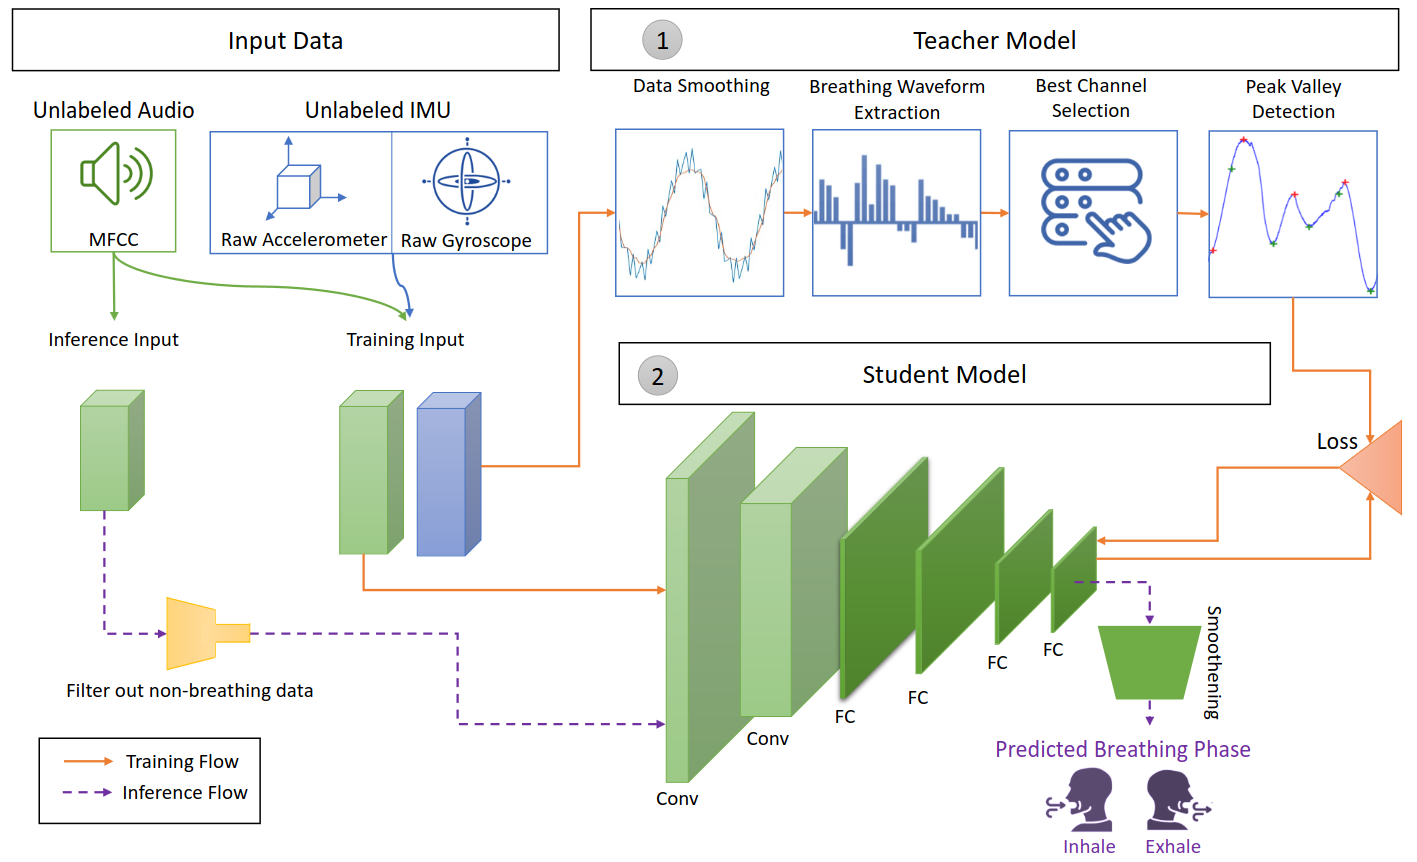
\includegraphics[width=0.90\linewidth]{obrazy/breathtrack_training_pipeline.png}
\caption{Potok treningu modelu BreathTrack, wykorzystujący architekturę Nauczyciel-Uczeń}
\label{fig:breathtrack_training_pipeline}
\end{figure}

Z kolei model predykcyjny dedykowany do docelowego działania opiera się wyłącznie na lekkiej, jednowymiarowej strukturze splotowej. Na wejście sieci trafiają 500 ms ramki dźwięku przetworzone do postaci współczynników melcepstralnych (MFCC). Architektura sieci składa się z dwóch warstw splotowych z normalizacją wsadową i 40-procentowym mechanizmem dropout. Następnie sygnał trafia do trzech warstw w pełni połączonych (FC) zakończonych funkcją aktywacji Sigmoid do klasyfikacji binarnej. Przez to że zrezygnowano tu ze struktur rekurencyjnych, w celu zachowania długofalowej spójności fizjologicznej autorzy zastosowali zewnętrzny algorytm wygładzania w fazie post-processingu. Analizuje on sąsiadujące segmenty czasowe i koryguje anomalie takie jak pojedynczy wdech wykryty w środku długiego wydechu znacząco poprawiając stabilność predykcji.

Ewaluacja systemu została przeprowadzona na zróżnicowanym zbiorze danych, obejmującym sesje nagraniowe w różnych pozycjach ciała i przy zmiennym natężeniu hałasu tła. Wyniki eksperymentalne wskazują, że BreathTrack osiąga dokładność w estymacji częstotliwości oddechu oraz granic faz oddechowych na poziomie porównywalnym z systemami w pełni nadzorowanymi, mimo braku dostępu do manualnych etykiet audio podczas treningu. Autorzy wykazali, iż błąd bezwzględny (MAE) w wyznaczaniu biomarkerów jest minimalny, co pozwala na wykorzystanie aplikacji do długofalowego monitorowania zdrowia, np. w wykrywaniu bezdechu sennego czy monitorowaniu stanów lękowych.

Z perspektywy projektowania systemów monitorujących oddech, BreathTrack rozwiązuje problem skalowalności. Po wytrenowaniu, model Ucznia jest w stanie analizować unikalną sygnaturę dźwiękową oddechu wyłącznie z mikrofonu, bez konieczności zakładania dodatkowych sensorów.

Należy jednak zauważyć pewne ograniczenia metodologiczne, które, podobnie jak w przypadku innych rozwiązań z tego segmentu, mogą wpływać na końcową ocenę pracy. Mianowicie autorzy nie zdecydowali się na upublicznienie kodu źródłowego ani zbioru danych, na którym przeprowadzano badania. Ogranicza to możliwość przeprowadzenia niezależnych testów porównawczych i utrudnia weryfikację odporności modelu na specyficzne, rzadkie artefakty akustyczne. Podsumowując, choć model jest w stanie wykryć nawet cichy oddech, jego wydajność w skrajnie głośnych środowiskach miejskich wciąż pozostaje obszarem wymagającym dalszego dostosowania.
\begin{comment}
Współczesne systemy mHealth kładą nacisk na interaktywność. Badania nad aplikacjami takimi jak te opisane w \textit{JMIR mHealth uHealth (doi:10.2196/63512)} oraz systemy typu \textbf{Breeze} (ACM, 10.1145/3369835), pokazują, że biofeedback oddechowy znacząco redukuje stres i poprawia uważność. Różnica między tymi rozwiązaniami a projektem dyplomowym polega na stopniu automatyzacji wykrywania faz – wiele rozwiązań komercyjnych wymaga ręcznego synchronizowania oddechu z animacją, podczas gdy niniejsza praca stawia na automatyczną detekcję.
\end{comment}
\subsection{Efektywne metody wizualizacji przebiegu treningu}
Kolejnym zagadnieniem w projektowaniu aplikacji wspierających treningi oddechowe jest sposób przekazywania użytkownikowi instrukcji dotyczących tempa i fazy oddechu. Tradycyjne metody wywodzące się z nagrań audio, opierają się wyłącznie na komendach głosowych. Obecnie popularniejszym podejściem są jednak metody wizualizujące oddech oraz przebieg treningu. Takie podejście zostało przebadane w artykule \textit{Evaluating mobile apps for breathing training: The effectiveness of visualization} \cite{chittaro2014evaluating}.

W ramach przeprowadzonych badań porównano trzy paradygmaty interfejsów aplikacji do treningu oddechowego. Każdy wariant został przetestowany dla treningu o docelowej częstotliwości sześciu cykli na minutę. Pierwszy z nich, wykorzystywał wyłącznie instrukcje głosowe z odliczaniem czasu trwania faz wdechu i wydechu. Następnie przebadano wariant widoczny na rysunku \ref{fig:sphere}, który integrował komunikaty audio z~pulsującą sferą, która rosła z wdechem, a także malała z wydechem, zmieniając przy tym kolor odpowiednio na zielony i czerwony. Trzeci wariant reprezentował podejście oparte na fali, w którym proces oddechu był wizualizowany jako przesuwająca się po ekranie fala trójkątna, z wyraźnie zaznaczonym bieżącym punktem cyklu, który widoczny jest na rysunku \ref{fig:wave}.

\begin{figure}[h]
    \centering
    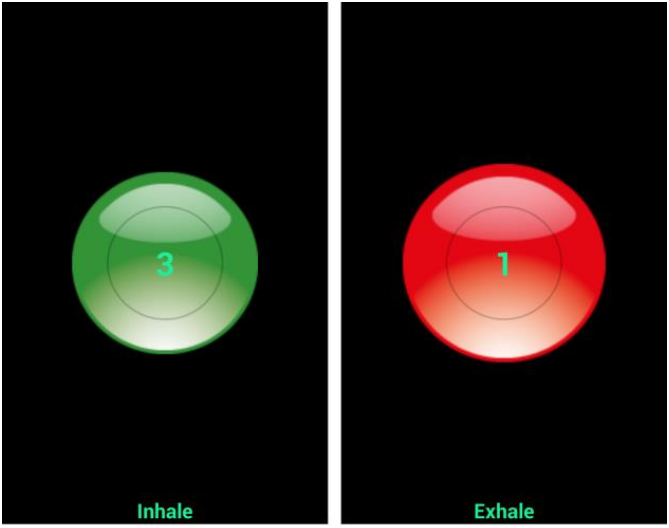
\includegraphics[width=0.80\linewidth]{obrazy/bubble.png}
    \caption{Wizualizacja treningu za pomocą sfery}
    \label{fig:sphere}
\end{figure}

\newpage

\begin{figure}[h]
    \centering
    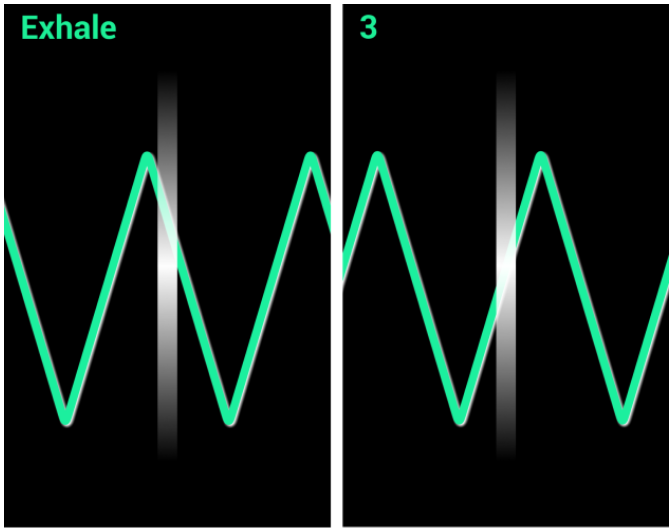
\includegraphics[width=0.80\linewidth]{obrazy/wave.png}
    \caption{Wizualizacja treningu za pomocą fali}
    \label{fig:wave}
\end{figure}

Ewaluacja przeprowadzona na grupie 68 uczestników przy użyciu klinicznej aparatury pomiarowej (m.in. sensorów objętości klatki piersiowej, czujników tętna oraz aktywności elektrodermalnej) jednoznacznie wykazała przewagę interfejsów wykorzystujących zaawansowaną wizualizację graficzną. Aplikacja wykorzystująca wizualizację fali pozwoliła użytkownikom na osiągnięcie statystycznie istotnie głębszego oddechu w docelowym paśmie częstotliwości w porównaniu do aplikacji bazującej wyłącznie na dźwięku.  

\begin{figure}[h]
    \centering
    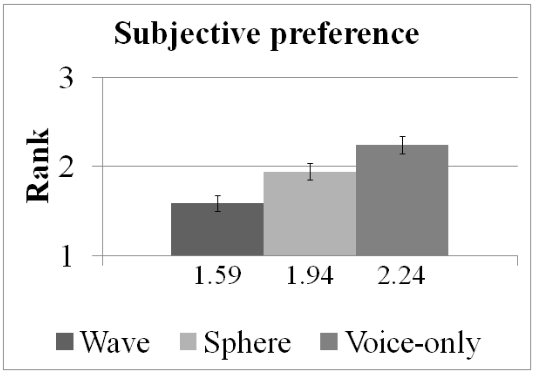
\includegraphics[width=0.5\linewidth]{obrazy/sub-pref.png}
    \caption{Porównanie wyników preferencji użytkowników w stosunku do sposoby wizualizacji treningu}
    \label{fig:sub-pref}
\end{figure}

Zaletą wizualizacji opartych na fali jest dostarczanie szerszego kontekstu czasowego ćwiczenia. W przeciwieństwie do pulsujących sfer lub komend głosowych, które informują jedynie o bieżącym stanie, fala na ekranie pozwala użytkownikowi obserwować zarówno aktualną, jak i~nadchodzącą fazę oddechu. Pozwala to na lepsze zaplanowanie objętości wdychanego powietrza i płynniejsze przejścia między fazami eliminując problem nagłego zatrzymywania oddechu przed końcem danej fazy z powodu braku pojemności płuc. Ponadto, jak wynika z rysunku \ref{fig:sub-pref} z~perspektywy subiektywnej oceny, użytkownicy ocenili wariant z falą jako najbardziej efektywny zarówno w kontekście nauki oddychania czy osiągania stanu relaksacji, wskazując go jako interfejs najbardziej preferowany.  

Wyniki te mają fundamentalne znaczenie dla projektowania systemów wspomagania treningów oddechu. Dowodzą one, że prawidłowo zaprojektowany wizualny biofeedback nie rozprasza użytkownika, lecz znacząco podnosi fizjologiczną skuteczność terapii. Wskazują również optymalny kierunek rozwoju interfejsów użytkownika, sugerując implementację grafów prezentujących ciągłość i historię cyklu oddechowego zamiast prostych animacji geometrycznych.
\begin{comment}
Wybór metody wizualizacji ma kluczowy wpływ na skuteczność treningu. Zgodnie z badaniami opublikowanymi w \textit{Computers in Human Behavior} (https://doi.org/10.1016/j.chb.2014.07.049):
\begin{itemize}
    \item \textbf{Wizualizacje abstrakcyjne (np. rozszerzające się koło):} Są najbardziej intuicyjne i najmniej obciążające poznawczo.
    \item \textbf{Wizualizacje oparte na naturze:} Zwiększają zaangażowanie i poczucie relaksacji (np. falowanie wody).
    \item \textbf{Wykresy w czasie rzeczywistym:} Najlepsze dla zaawansowanych użytkowników i celów diagnostycznych, ale mogą powodować stres u osób początkujących.
\end{itemize}
Zaleca się stosowanie płynnych przejść tonalnych i organicznych kształtów, aby uniknąć efektu "mechanicznego" narzucania rytmu.
\end{comment}

\section{Narzędzia i środowiska do tworzenia aplikacji mobilnych}
Tworzenie osobnych aplikacji dla systemów Android i iOS zapewnia pełny dostęp do funkcji oferowanych przez daną platformę, wymaga jednak utrzymywania dwóch baz kodu oraz znajomości odmiennych technologii. Rozwiązania wieloplatformowe ograniczają ten koszt przez współdzielenie logiki biznesowej, warstwy interfejsu lub obu tych elementów. Poszczególne narzędzia różnią się sposobem renderowania interfejsu, zakresem współdzielenia kodu czy metodą komunikacji z natywnymi interfejsami programistycznymi systemu.

\subsection{Flutter}
Flutter jest rozwijanym przez Google otwartoźródłowym zestawem narzędzi wykorzystującym język Dart. Umożliwia tworzenie aplikacji dla systemów Android i iOS, a także dla platform internetowych, desktopowych oraz wbudowanych, z wykorzystaniem jednej bazy kodu \cite{flutterDocs2026}. Interfejs użytkownika jest budowany deklaratywnie z hierarchii widżetów i renderowany przez mechanizmy dostarczane przez framework. Takie podejście ułatwia zachowanie spójnego wyglądu aplikacji na różnych urządzeniach oraz tworzenie niestandardowych animacji. Mechanizm \textit{Hot Reload} pozwala ponadto obserwować większość zmian bez ponownego uruchamiania aplikacji, co skraca cykl implementacji i testowania interfejsu.

Flutter udostępnia gotowe widżety zgodne m.in. ze stylami Material Design i Cupertino, które zapewniają nowoczesny wygląd oraz pozytywne doświadczenie z użytkowania aplikacji. Dostęp do czujników, mikrofonu, systemu plików oraz pozostałych funkcji urządzenia jest realizowany za pośrednictwem importu odpowiednich wtyczek. Jeżeli wymaganej funkcji nie zapewnia istniejący już pakiet, możliwe jest wywołanie kodu napisanego dla konkretnej platformy, np. w języku Kotlin dla systemu Android lub Swift dla systemu iOS, za pomocą kanałów platformowych \cite{flutterPlatformChannels2026}. Wadą tego rozwiązania może być konieczność utrzymywania dodatkowego kodu natywnego dla rzadziej wykorzystywanych funkcji urządzenia. Flutter stanowi szczególnie użyteczną technologię w aplikacjach wymagających spójnego wyglądu interfejsu dla wielu platform oraz płynnych wizualizacji przy minimalnej potrzebie dostosowywania kodu do poszczególnych platform.

\subsection{React Native}
Konkurencyjnym rozwiązaniem do tworzenia aplikacji wieloplatformowych jest React Native. Jest to otwartoźródłowy framework wykorzystujący React oraz język JavaScript lub TypeScript. React Native zachowuje komponentowy model tworzenia interfejsu znany z biblioteki React \cite{reactComponents2026}, natomiast jego podstawowe komponenty są odwzorowywane na elementy interfejsu właściwe dla platformy docelowej \cite{reactNativeDocs2026}. Pozwala to współdzielić znaczną część kodu przy zachowaniu sposobu działania i wyglądu zbliżonego do aplikacji natywnych. Framework ten może być również rozszerzeniem do istniejących już aplikacji napisanych w języku Kotlin lub Swift. Daje on możliwość dodania pojedynczych widoków lub widżetów.

W przypadku nowych aplikacji dokumentacja React Native zaleca korzystanie z frameworka uzupełniającego, takiego jak Expo, który dostarcza między innymi routing, biblioteki obsługujące funkcje urządzenia i narzędzia budowania aplikacji \cite{reactNativeGettingStarted2026}. Zaletami React Native są rozbudowany ekosystem pakietów oraz możliwość wykorzystania wiedzy oraz części narzędzi znanych z programowania aplikacji internetowych. Ograniczeniem może być zależność od zgodności bibliotek z aktualną architekturą frameworka. Implementacja nietypowych funkcji lub integracja specjalistycznego przetwarzania sygnałów może ponadto wymagać przygotowania modułów natywnych oddzielnie dla systemów Android i iOS.

\subsection{Kotlin Multiplatform}
Kotlin Multiplatform umożliwia współdzielenie kodu w języku Kotlin pomiędzy systemami Android i iOS, a także platformami desktopowymi, internetowymi i serwerowymi \cite{kotlinMultiplatform2026}. W odróżnieniu od frameworków narzucających jeden sposób tworzenia całej aplikacji programista może zdecydować, które warstwy będą wspólne. Typowym rozwiązaniem jest współdzielenie modeli danych, komunikacji sieciowej i logiki biznesowej przy pozostawieniu natywnych interfejsów użytkownika. Zastosowanie Compose Multiplatform pozwala dodatkowo współdzielić także warstwę interfejsu.

Podejście to zapewnia dużą elastyczność oraz bezpośredni dostęp do mechanizmów poszczególnych platform. Jest korzystne zwłaszcza wtedy, gdy istotne jest zachowanie natywnego interfejsu lub gdy projekt ma być rozwijany stopniowo na podstawie istniejącej aplikacji. Ceną tej elastyczności jest bardziej złożona struktura projektu, a także możliwa konieczność równoczesnego korzystania z narzędzi Android Studio oraz Xcode. Kotlin Multiplatform nie zawsze eliminuje więc potrzebę znajomości obu platform, lecz pozwala ograniczyć powielanie najważniejszej logiki aplikacji.

\subsection{Pozostałe rozwiązania}
Alternatywę dla opisanych technologii stanowi .NET Multi-platform App UI (.NET MAUI). W tym frameworku aplikacje tworzy się w języku C\#, natomiast interfejs użytkownika może być definiowany za pomocą języka znaczników XAML. Framework pozwala współdzielić logikę oraz interfejs aplikacji przeznaczonych dla systemów Android, iOS, macOS i Windows, zachowując możliwość dołączenia kodu specyficznego dla platformy \cite{dotnetMaui2026}. Jego zaletą jest integracja z ekosystemem .NET i środowiskiem Visual Studio, natomiast mniejsze znaczenie ma w projektach niezwiązanych z technologiami Microsoftu.

Innym podejściem jest Ionic, w którym interfejs powstaje z wykorzystaniem HTML, CSS i JavaScript oraz może być łączony z frameworkami Angular, React lub Vue. Aplikacja może działać jako aplikacja internetowa PWA, a środowisko Capacitor umożliwia jej uruchamianie na urządzeniach mobilnych i dostęp do funkcji natywnych \cite{ionicDocs2026}. Rozwiązanie to ułatwia przeniesienie istniejącej aplikacji internetowej na urządzenia mobilne. Warstwa oparta na technologiach webowych może jednak stanowić ograniczenie w projektach wymagających szczególnie intensywnych animacji, przetwarzania danych w czasie rzeczywistym lub ścisłej integracji ze sprzętem.
\subsection{Podsumowanie}
Wybór narzędzia powinien uwzględniać nie tylko procent współdzielonego kodu, ale również dostępność wymaganych bibliotek, jakość obsługi czujników i mikrofonu, wydajność animacji, kompetencje zespołu oraz przewidywany koszt utrzymania modułów natywnych. W przypadku aplikacji wspomagającej trening oddechowy istotne są zwłaszcza stabilne pozyskiwanie dźwięku, wykonywanie obliczeń w czasie rzeczywistym oraz płynna synchronizacja wizualizacji z wykrytą fazą oddechu. Flutter oferuje w tym zakresie dużą kontrolę nad spójnym interfejsem i animacjami, natomiast React Native ułatwia wykorzystanie ekosystemu JavaScript, a także bardziej intuicyjną pracę z kodem dla dla deweloperów aplikacji internetowych. Kotlin Multiplatform jest z kolei odpowiedni, gdy priorytetem pozostaje zachowanie natywnej warstwy interfejsu przy współdzieleniu algorytmów i logiki biznesowej.

\section{Narzędzia do wdrażania modeli AI na urządzeniach mobilnych}

Model wytrenowany w środowisku takim jak TensorFlow lub PyTorch nie powinien być bezpośrednio umieszczany w aplikacji mobilnej. Frameworki wykorzystywane podczas uczenia zawierają funkcje, które nie są potrzebne do wykonywania predykcji, a ich pełne środowiska wykonawcze są zbyt rozbudowane dla urządzeń o ograniczonej pamięci i mocy obliczeniowej. Typowy proces wdrożenia obejmuje zapis grafu obliczeniowego modelu, konwersję do formatu obsługiwanego przez mobilne środowisko wykonawcze, optymalizację, dołączenie pliku modelu do aplikacji oraz przeprowadzenie testów na urządzeniu docelowym.

\subsection{ONNX i ONNX Runtime Mobile}

Open Neural Network Exchange (ONNX) jest otwartym formatem reprezentacji modeli uczenia maszynowego. Model jest zapisywany jako graf, którego węzły opisują operacje matematyczne, natomiast krawędzie określają przepływ tensorów pomiędzy operacjami. Celem formatu jest uniezależnienie etapu wdrożenia od frameworka wykorzystanego do uczenia modelu \cite{onnxConcepts2026}. Przykładowo model przygotowany w PyTorch może zostać wyeksportowany do pliku \texttt{.onnx}, a~następnie uruchomiony bez obecności pełnego środowiska PyTorch.

Sam ONNX definiuje sposób zapisu modelu, lecz nie jest mobilnym silnikiem wnioskowania. Do wykonywania predykcji może służyć ONNX Runtime Mobile, dostępny dla systemów Android i iOS \cite{onnxRuntimeMobile2026}. Środowisko analizuje graf oraz dobiera implementacje operatorów odpowiednie dla procesora głównego lub dostępnego akceleratora. Model można dodatkowo przekonwertować do formatu ORT, jak również zbudować środowisko zawierające jedynie używane operatory, ograniczając rozmiar biblioteki dołączanej do aplikacji. Zaletą tego rozwiązania jest możliwość utrzymywania jednego formatu modelu dla obu głównych platform mobilnych. Ograniczeniem może być brak obsługi niektórych niestandardowych operatorów albo konieczność dostosowania wersji zestawu operatorów użytego podczas eksportu.

ONNX Runtime udostępnia również narzędzia do kwantyzacji statycznej i dynamicznej. Pozwalają one zastąpić część obliczeń wykonywanych na liczbach 32-bitowych operacjami wykorzystującymi liczby 8-bitowe \cite{onnxQuantization2026}. Zmniejsza to rozmiar wag oraz zapotrzebowanie na pamięć, a na obsługiwanym sprzęcie może także skrócić czas predykcji. Kwantyzacja może jednak powodować pogorszenie jakości wyników, z tego powodu model po optymalizacji musi zostać ponownie oceniony na reprezentatywnym zbiorze danych.

\subsection{TensorFlow Lite i LiteRT}

TensorFlow Lite jest rozwiązaniem przeznaczonym do uruchamiania modeli na urządzeniach mobilnych i brzegowych. Obecnie technologia ta jest rozwijana przez Google pod nazwą LiteRT, przy zachowaniu obsługi istniejących modeli oraz interfejsu TensorFlow Lite Interpreter \cite{liteRTMigration2026}. Podstawowym formatem pozostaje plik \texttt{.tflite}, będący zoptymalizowaną reprezentacją modelu opartą na formacie FlatBuffer. Modele przygotowane w TensorFlow można konwertować z formatu SavedModel lub bezpośrednio z obiektu Keras. LiteRT obsługuje również ścieżki konwersji modeli utworzonych w PyTorch i JAX \cite{liteRTOverview2026}.

Proces konwersji pozwala zastosować między innymi kwantyzację wag i aktywacji, dołączyć metadane opisujące wejścia i wyjścia oraz określić sposób obsługi niestandardowych operatorów \cite{liteRTConversion2026}. Podczas wykonywania predykcji środowisko może korzystać z procesora CPU, GPU lub NPU, zależnie od systemu oraz możliwości urządzenia. LiteRT jest rozwiązaniem wieloplatformowym, jednak szczególnie dobrze integruje się z aplikacjami dla systemu Android. Ważnym ograniczeniem jest to, że mobilny zestaw operatorów jest mniejszy niż pełny zestaw TensorFlow. Model wykorzystujący nieobsługiwaną operację może wymagać zmiany architektury, zastosowania operatora niestandardowego lub dołączenia rozszerzonego środowiska wykonawczego.

\subsection{Core ML}

Core ML jest środowiskiem firmy Apple przeznaczonym do integracji modeli uczenia maszynowego z aplikacjami dla systemów iOS, iPadOS, macOS i pozostałych platform Apple. Model dołącza się do projektu Xcode w formacie \texttt{.mlmodel} lub pakietu modelu, a Xcode generuje interfejs programistyczny ułatwiający przekazywanie danych wejściowych, jak również odczytywanie predykcji \cite{coreMLIntegration2026}. System może wykonywać obliczenia z wykorzystaniem CPU, GPU oraz układu Neural Engine, dobierając zasoby dostępne na urządzeniu.

Narzędzie Core ML Tools umożliwia konwersję modeli pochodzących między innymi z PyTorch i TensorFlow oraz zmianę typów oraz kształtów danych wejściowych \cite{coreMLTools2026}. Dostępne są także techniki optymalizacji, takie jak kwantyzacja, przycinanie wag i paletyzacja. Core ML zapewnia ścisłą integrację z ekosystemem Apple, a także może oferować bardzo dobrą efektywność na urządzeniach tej firmy, nie jest jednak rozwiązaniem wieloplatformowym. W projekcie obsługującym Androida i iOS zastosowanie Core ML oznacza zatem utrzymywanie oddzielnego wariantu modelu lub oddzielnej ścieżki eksportu dla platform Apple.

\subsection{ExecuTorch}

ExecuTorch jest częścią ekosystemu PyTorch przeznaczoną do wykonywania wnioskowania na telefonach, urządzeniach ubieralnych i systemach wbudowanych \cite{execuTorch2026}. Proces wdrożenia rozpoczyna się od eksportu programu PyTorch do grafu za pomocą mechanizmów \texttt{torch.export}. Graf jest następnie optymalizowany oraz kompilowany do programu ExecuTorch zapisywanego zazwyczaj w pliku \texttt{.pte}. Lekki runtime uruchamia przygotowany program na urządzeniu docelowym.

Podczas przygotowania modelu możliwe jest wskazanie backendu wykorzystującego określony rodzaj sprzętu, np. XNNPACK dla CPU, Core ML lub Metal Performance Shaders na urządzeniach Apple, a także rozwiązania dostawców mobilnych układów NPU \cite{execuTorchExport2026}. ExecuTorch jest szczególnie użyteczny, gdy model powstaje w PyTorch, jak również wymagane jest zachowanie spójnego zestawu narzędzi od treningu do wdrożenia. W zależności od docelowych urządzeń może być jednak konieczne wygenerowanie osobnych, zoptymalizowanych plików programu dla różnych backendów sprzętowych.

\subsection{Dobór formatu i optymalizacja modelu}

Wybór technologii wdrożeniowej zależy od frameworka treningowego, platform docelowych i~rodzaju wykorzystywanej akceleracji. ONNX Runtime Mobile jest korzystny, gdy istotna jest przenośność pomiędzy frameworkami oraz wspólny format dla Androida oraz iOS. LiteRT stanowi naturalny wybór dla modeli TensorFlow oraz aplikacji silnie związanych z ekosystemem Androida. Core ML pozwala najlepiej wykorzystać mechanizmy platform Apple, natomiast ExecuTorch zapewnia bezpośrednią ścieżkę wdrażania modeli rozwijanych w PyTorch.

Niezależnie od wybranego formatu proces optymalizacji powinien obejmować porównanie wyników modelu przed konwersją i po niej, pomiar czasu pojedynczej predykcji, zużycia pamięci, rozmiaru pliku oraz poboru energii. Testy należy wykonywać na rzeczywistych urządzeniach, ponieważ wyniki uzyskane na komputerze lub emulatorze nie odzwierciedlają działania mobilnych akceleratorów. W aplikacji analizującej oddech szczególnie ważne jest również zachowanie identycznego przetwarzania wstępnego sygnału. Długość okna czasowego, częstotliwość próbkowania, normalizacja oraz sposób obliczania cech, takich jak MFCC lub spektrogram log-mel, muszą odpowiadać parametrom użytym podczas treningu. Rozbieżność w tym zakresie może obniżyć skuteczność klasyfikacji nawet wtedy, gdy sama konwersja modelu przebiegła poprawnie.

\section{Pozyskiwanie i reprezentacja sygnału oddechowego}

Pozyskiwanie sygnału oddechowego poza środowiskiem klinicznym może być realizowane z wykorzystaniem czujników powszechnie dostępnych w smartfonach. Należy jednak rozróżnić bezpośrednią rejestrację zjawiska związanego z przepływem powietrza od pomiarów pośrednich. Mikrofon rejestruje dźwięk powstający podczas wdechu i wydechu, natomiast akcelerometr, żyroskop, a także kamera pozwalają obserwować ruchy ciała lub modulacje sygnału krążeniowego wywołane oddychaniem. Czujniki telefonu nie mierzą bezpośrednio objętości oddechowej ani przepływu powietrza tak jak spirometr, dlatego wyniki uzyskiwane za ich pomocą mają zwykle postać estymowanej częstotliwości oddychania, faz cyklu czy cech jakościowych.

\subsection{Mikrofon}

Mikrofon jest najbardziej naturalnym czujnikiem dla aplikacji, której zadaniem jest rozpoznawanie wdechu, wydechu i pauzy. Rejestrowany sygnał zawiera szum przepływu powietrza w~obrębie nosa oraz ust, dźwięki pochodzące z dróg oddechowych oraz zakłócenia otoczenia. Telefon może znajdować się przed twarzą użytkownika, obok łóżka lub w ustalonej pozycji wykorzystywanej podczas ćwiczenia. Nie wymaga to kontaktu ze skórą ani dodatkowego wyposażenia, a~wcześniejsze systemy Breeze i BreathTrack potwierdzają możliwość analizy faz oddechu za pomocą mikrofonu smartfona \cite{10.1145/3369835,10.1145/3478123}.

Jakość danych akustycznych silnie zależy od odległości i orientacji telefonu, charakterystyki mikrofonu, automatycznej regulacji wzmocnienia oraz obecności mowy, muzyki, wentylacji czy innych dźwięków. Szczególnie trudna jest detekcja naturalnego wdechu, który może mieć niewielką amplitudę. Z tego względu protokół rejestracji powinien określać położenie urządzenia, częstotliwość próbkowania, długość nagrania oraz warunki akustyczne. W aplikacji działającej w~czasie rzeczywistym warto dodatkowo wykrywać fragmenty o niewystarczającej jakości i informować użytkownika o konieczności zmiany położenia telefonu.

\subsection{Czujniki inercyjne}

Akcelerometr oraz żyroskop tworzą układ IMU, który pozwala obserwować niewielkie przemieszczenia i zmiany orientacji telefonu wywołane ruchem klatki piersiowej lub brzucha. W najprostszym wariancie urządzenie jest położone na tułowiu albo utrzymywane w stałym kontakcie z ciałem. Składowa oddechowa jest następnie oddzielana od grawitacji, ruchów kończyn, a także innych zakłóceń. W badaniu Lee i Yoo częstotliwość oddychania estymowano na podstawie trójosiowego akcelerometru smartfona, wykorzystując filtrację, analizę składowych niezależnych i analizę cepstralną \cite{lee2020smartphoneRespiration}.

Zaletą IMU jest brak wpływu hałasu akustycznego oraz możliwość uzyskania wyraźnego, okresowego przebiegu podczas spokojnego oddychania. Ograniczeniem jest konieczność stabilnego położenia telefonu. Zmiana pozycji ciała, chodzenie, ruch ręki lub drgania podłoża mogą mieć amplitudę wielokrotnie większą od sygnału oddechowego. Częstotliwość próbkowania czujników może ponadto różnić się pomiędzy modelami urządzeń oraz nie zawsze jest idealnie stała, dlatego próbki powinny zawierać znaczniki czasu i być przeskalowane do wspólnej osi czasowej.

\subsection{Kamera}

Kamera smartfona umożliwia dwie odmienne metody pomiaru. Pierwsza polega na bezkontaktowej obserwacji górnej części tułowia. Z kolejnych klatek filmu wyznaczane jest przemieszczenie klatki piersiowej, jak również brzucha, np. za pomocą przepływu optycznego, śledzenia punktów charakterystycznych albo zmian intensywności wybranego obszaru obrazu. Badania z wykorzystaniem przedniej kamery telefonu wykazały możliwość estymacji częstotliwości oddechu na podstawie ruchów tułowia \cite{nam2016dualCamera,bae2022smartphoneCameraRespiration}. Metoda wymaga jednak stabilnej kamery, odpowiedniego oświetlenia i~ograniczenia ruchów niezwiązanych z oddychaniem.

Drugi wariant wykorzystuje fotopletyzmografię obrazową. Użytkownik przykłada palec do tylnej kamery, zwykle przy włączonej diodzie, a zmiany jasności kolejnych klatek odzwierciedlają zmiany objętości krwi. Oddychanie moduluje amplitudę oraz częstotliwość sygnału PPG, dzięki czemu można pośrednio oszacować częstość oddechów \cite{nam2014cameraRespiration}. Rozwiązanie to nie rejestruje dźwięku ani ruchu klatki piersiowej i zazwyczaj lepiej nadaje się do wyznaczania częstotliwości niż dokładnych granic pomiędzy wdechem, wydechem czy pauzą.

\subsection{Łączenie wielu źródeł danych}

Sygnały z różnych czujników mogą być łączone w celu zwiększenia odporności systemu. Mikrofon może dostarczać informacji o charakterze i fazie dźwięku, podczas gdy IMU lub kamera stanowią niezależne potwierdzenie ruchu oddechowego. Fuzja może odbywać się na poziomie cech, przez połączenie wektorów wejściowych, albo na poziomie decyzji, przez zestawienie predykcji osobnych modeli. Takie rozwiązanie zwiększa jednak złożoność aplikacji, a także wymaga dokładnej synchronizacji strumieni o różnych częstotliwościach próbkowania. W praktyce czujnik dodatkowy może być również używany wyłącznie podczas pozyskiwania zbioru treningowego jako źródło etykiet referencyjnych, takich jak dane inercyjne wykorzystane do automatycznego oznaczania dźwięku w systemie BreathTrack \cite{10.1145/3478123}.

\subsection{Reprezentacje sygnału}

Sposób reprezentacji danych powinien zachowywać informacje potrzebne do realizowanego zadania, a jednocześnie ograniczać wpływ zakłóceń i różnic pomiędzy urządzeniami. W~przypadku dźwięku punktem wyjścia jest jednowymiarowy przebieg amplitudy PCM. Może on zostać przekazany bezpośrednio do modelu analizującego surową falę albo podzielony na zachodzące na siebie ramki. Z ramek wyznacza się podstawowe cechy czasowe, takie jak energia, wartość RMS, obwiednia amplitudy oraz liczba przejść przez zero. Cechy te są tanie obliczeniowo, lecz mają ograniczoną zdolność rozróżniania oddechu od dźwięków o podobnym poziomie energii.

Najczęściej stosowane reprezentacje czasowo-częstotliwościowe oblicza się za pomocą STFT (ang. \textit{short-time Fourier transform}). Wynikiem jest spektrogram opisujący zmianę energii w pasmach częstotliwości w czasie. Po przeliczeniu częstotliwości na skalę mel i zastosowaniu logarytmu otrzymuje się spektrogram log-mel, natomiast dalsza transformacja prowadzi do współczynników melcepstralnych MFCC. Reprezentacje log-mel oraz MFCC ograniczają wymiar danych oraz dobrze współpracują z sieciami CNN, RNN i modelami hybrydowymi. Były one wykorzystywane m.in. w systemach Breeze i BreathTrack \cite{10.1145/3369835,10.1145/3478123}. Alternatywę stanowią reprezentacje uczone automatycznie, np. wektory uzyskane z modeli audio wstępnie wytrenowanych na dużych zbiorach dźwięków.

Dane z IMU mają postać wielokanałowych szeregów czasowych zawierających trzy osie przyspieszenia, a także trzy osie prędkości kątowej. Przed analizą zwykle wykonuje się interpolację do stałej częstotliwości próbkowania, usunięcie składowej grawitacyjnej i filtrację w paśmie odpowiadającym oddychaniu. Reprezentacją wejściową może być pełny zestaw osi, moduł wektora, dominująca składowa uzyskana metodą PCA lub ICA, widmo częstotliwościowe albo sekwencja krótkich okien czasowych. W danych wizyjnych obraz jest najpierw redukowany do obszaru zainteresowania, a następnie przekształcany w jednowymiarowy przebieg ruchu, sekwencję wektorów przepływu optycznego albo przebieg zmian barwy odpowiadający PPG.

Dla klasyfikacji faz oddechu etykieta powinna być przypisana do każdej ramki lub przedziału czasu i określać co najmniej wdech, wydech oraz pauzę. Innym zadaniem jest estymacja częstotliwości oddechu, w której wynik stanowi liczba cykli na minutę, lub klasyfikacja całego nagrania, np. jako oddechu prawidłowego albo patologicznego. Zbiory przygotowane do jednego z tych zadań nie zawsze mogą być bezpośrednio użyte w innym, ponieważ etykieta choroby lub rodzaju nagrania nie zawiera informacji o dokładnych granicach faz.

\subsection{Dostępne zbiory danych}

Publicznie dostępne dane oddechowe różnią się rodzajem czujnika, protokołem rejestracji i~szczegółowością adnotacji. Do najczęściej wykorzystywanych zbiorów należą:

\begin{itemize}
    \item \textbf{ICBHI 2017 Respiratory Sound Database} zawiera 920 nagrań pochodzących od 126 osób, obejmujących łącznie około 5,5 godziny oraz 6898 oznaczonych cykli oddechowych. Adnotacje wskazują obecność prawidłowych cykli, trzeszczeń i świstów \cite{rocha2019respiratoryDatabase}. Nagrania wykonano za pomocą różnych urządzeń osłuchowych, dlatego zbiór dobrze nadaje się do analizy dźwięków płuc, ale jego charakterystyka różni się od dźwięku rejestrowanego mikrofonem telefonu znajdującego się przed twarzą.

    \item \textbf{Coswara} obejmuje około 65 godzin nagrań zebranych od 2635 uczestników za pomocą aplikacji internetowej dostępnej ze smartfonów oraz komputerów. Każdy rekord może zawierać oddech głęboki i płytki, kaszel, samogłoski oraz mowę, a także dane demograficzne, objawy oraz status testu SARS-CoV-2 \cite{bhattacharya2023coswara}. Zbiór jest zbliżony do rzeczywistych warunków użycia mikrofonu konsumenckiego, lecz etykiety opisują typ całego nagrania, jak również stan uczestnika, a nie dokładne granice wdechów i wydechów.

    \item \textbf{COVID-19 Sounds} Uniwersytetu Cambridge zawiera nagrania kaszlu, oddychania, a także mowy zbierane za pomocą aplikacji mobilnej wraz z ankietą oraz wynikiem testu. W opublikowanych eksperymentach wykorzystano 5240 próbek od 2478 uczestników \cite{han2022covidSounds}. Zbiór jest przydatny do badań nad danymi rejestrowanymi w niekontrolowanym środowisku, ale podobnie jak Coswara został przygotowany głównie do klasyfikacji stanu zdrowia, a nie segmentacji cyklu oddechowego.

    \item \textbf{HF\_Lung\_V1} zawiera 9765 piętnastosekundowych nagrań wykonanych cyfrowym stetoskopem. Udostępnia dziesiątki tysięcy oznaczeń wdechu i wydechu oraz adnotacje świstów, trzeszczeń czy innych dźwięków dodatkowych \cite{hsu2021hfLung}. Szczegółowe etykiety faz są cenne podczas budowy modeli sekwencyjnych, jednak różnica miejsca i sposobu rejestracji powoduje, że model wytrenowany na tym zbiorze wymaga adaptacji oraz walidacji na nagraniach z mikrofonu smartfona.

    \item \textbf{BIDMC PPG and Respiration Dataset} udostępniony w serwisie PhysioNet składa się z 53 ośmiominutowych rekordów pacjentów intensywnej terapii. Każdy rekord zawiera PPG, EKG, sygnał oddechowy z~pneumografii impedancyjnej, parametry życiowe oraz ręczne oznaczenia oddechów \cite{bidmcRespirationDataset}. Zbiór nie pochodzi ze smartfonów, ale umożliwia opracowywanie i ocenę algorytmów wyznaczających oddech pośrednio z sygnału PPG, który może być również rejestrowany za pomocą kamery telefonu.
\end{itemize}

\begin{table}[htbp]
    \centering
    \caption{Porównanie publicznie dostępnych zbiorów danych oddechowych}
    \label{tab:respiratory_datasets}
    \footnotesize
    \setlength{\tabcolsep}{4pt}
    \renewcommand{\arraystretch}{1.1}
    \begin{tabularx}{\textwidth}{@{}p{2cm}p{2.4cm}p{2.5cm}p{2.1cm}X@{}}
        \toprule
        \textbf{Zbiór} & \textbf{Sygnał} & \textbf{Osoby / próbki} & \textbf{Czas nagrań} & \textbf{Adnotacje} \\
        \midrule
        ICBHI 2017 \cite{rocha2019respiratoryDatabase}
        & Stetoskop elektroniczny
        & 126 osób, 920 nagrań
        & 10--90 s; łącznie ok. 5,5 h
        & 6898 cykli; oddech prawidłowy, trzeszczenia i świsty \\
        \midrule

        Coswara \cite{bhattacharya2023coswara}
        & Mikrofon telefonu lub komputera
        & 2635 osób, ok. 23 700 próbek
        & Łącznie ok. 65 h
        & Oddech, kaszel, mowa, objawy i status zdrowotny \\
        \midrule

        COVID-19 Sounds \cite{han2022covidSounds}
        & Mikrofon telefonu
        & 2478 osób, 5240 próbek
        & Zmienny
        & Oddech, kaszel, mowa, objawy i wynik testu \\
        \midrule

        HF\_Lung\_V1 \cite{hsu2021hfLung}
        & Cyfrowy stetoskop, 4 kHz
        & 279 osób, 9765 nagrań
        & 15 s każde; łącznie ok. 40,7 h
        & Wdechy, wydechy i dodatkowe dźwięki oddechowe \\
        \midrule

        BIDMC \cite{bidmcRespirationDataset}
        & PPG, EKG i pneumografia impedancyjna
        & 53 osoby, 53 rekordy
        & 8 min każdy; łącznie ok. 7,1 h
        & Oznaczenia oddechów i parametry życiowe \\
        \bottomrule
    \end{tabularx}
\end{table}

\subsubsection{Podsumowanie}
Dostępne zbiory nie rozwiązują w pełni problemu detekcji faz naturalnego oddechu za pomocą mikrofonu telefonu. Bazy osłuchowe oferują dokładne etykiety, lecz reprezentują inną domenę akustyczną, natomiast duże zbiory crowdsourcingowe zawierają dźwięk ze smartfonów, ale przeważnie nie mają adnotacji czasowych faz. Dane zebrane dla Breeze i BreathTrack nie zostały publicznie udostępnione wraz z kodem i etykietami \cite{10.1145/3369835,10.1145/3478123}. Z tego względu dla projektowanego systemu uzasadnione jest utworzenie własnego zbioru, nagranego w warunkach odpowiadających docelowemu użyciu aplikacji.

Podczas tworzenia takiego zbioru dźwięk z mikrofonu powinien być rejestrowany równocześnie z sygnałem referencyjnym, np. z pasa oddechowego, czujnika przepływu lub odpowiednio zamocowanego IMU. Pozwala to automatycznie albo półautomatycznie wyznaczyć granice wdechu, wydechu i pauzy. Podział na zbiory treningowy, walidacyjny oraz testowy należy przeprowadzać według uczestników, a nie pojedynczych fragmentów nagrania, aby próbki tej samej osoby nie występowały po obu stronach oceny. Wskazane jest również uwzględnienie różnych modeli telefonów, odległości od mikrofonu, pozycji ciała oraz kontrolowanych rodzajów hałasu. Tak przygotowane dane lepiej odzwierciedlają warunki działania aplikacji niż samo połączenie istniejących baz o odmiennych protokołach rejestracji.

\newpage

\section{Istniejące rozwiązania klasyfikacji faz oddechu}

Analiza sygnału oddechowego może prowadzić do kilku różnych zadań. Klasyfikacja całego nagrania przypisuje mu jedną etykietę, np. oddech prawidłowy, świst lub trzeszczenie. Detekcja zdarzeń wskazuje przedziały czasu, w których występują określone dźwięki. Najbardziej szczegółowym zadaniem jest segmentacja faz, polegająca na przypisaniu każdej ramce sygnału etykiety wdechu, wydechu albo pauzy. Rozróżnienie tych problemów jest istotne, ponieważ model osiągający wysoką skuteczność klasyfikacji całych cykli nie musi poprawnie wyznaczać momentów przejścia pomiędzy fazami.

\subsection{Metody progowe i klasyczne uczenie maszynowe}

Najprostsze algorytmy wykorzystują obwiednię amplitudy, energię krótkoczasową, liczbę przejść przez zero lub moc sygnału w wybranych pasmach częstotliwości. Po wygładzeniu przebiegu stosuje się progi decyzyjne, wykrywanie maksimów i minimalny dopuszczalny czas trwania fazy. Metody te mają niewielkie wymagania obliczeniowe oraz mogą działać bezpośrednio na urządzeniu mobilnym. Ich skuteczność silnie zależy jednak od poziomu głośności, położenia mikrofonu i~hałasu otoczenia. Próg dobrany dla jednego użytkownika lub urządzenia może być nieodpowiedni dla innych nagrań.

Bardziej rozbudowane rozwiązania klasyczne wyznaczają wektor cech zawierający m.in. MFCC, energię pasmową, parametry widmowe oraz charakterystyki obwiedni. Następnie wykorzystują klasyfikatory takie jak regresja logistyczna, maszyna wektorów nośnych, las losowy lub ukryty model Markowa. Modele sekwencyjne, np. HMM, pozwalają uwzględnić fakt, że fazy oddechu występują w określonej kolejności. Zaletą klasycznych metod jest łatwiejsza interpretacja oraz możliwość uczenia na mniejszej liczbie przykładów. Ograniczeniem pozostaje konieczność ręcznego projektowania cech oraz reguł przejścia, które nie zawsze opisują zróżnicowane wzorce oddechowe.

\subsection{Splotowe sieci neuronowe}

Splotowe sieci neuronowe (CNN) automatycznie uczą się lokalnych wzorców występujących w sygnale. Jednowymiarowe sieci CNN mogą analizować bezpośrednio przebieg amplitudy albo sekwencję cech akustycznych. Sieci dwuwymiarowe otrzymują zazwyczaj spektrogram lub spektrogram log-mel, który jest traktowany jak obraz. Filtry splotowe wykrywają w nim lokalne zmiany energii, pasma częstotliwości oraz krótkie struktury charakterystyczne dla wdechu i wydechu.

W jednowymiarowej sieci filtr jest przesuwany wzdłuż osi czasu i reaguje np. na nagły wzrost energii, rytmiczne zmiany amplitudy lub strukturę szumu oddechowego. W sieci dwuwymiarowej filtr obejmuje jednocześnie fragment czasu i zakres częstotliwości, dzięki czemu może wykrywać lokalne kształty na spektrogramie. Pierwsze warstwy uczą się prostych wzorców, natomiast kolejne łączą je w bardziej złożone reprezentacje fazy. Operacje redukcji rozmiaru, takie jak pooling albo splot z krokiem większym od jedności, zmniejszają liczbę danych i zwiększają zakres sygnału widoczny dla kolejnych warstw. Ostatnia głowica klasyfikacyjna przekształca wyuczone cechy w predykcję klasy dla całego okna lub kolejnych ramek.

Autorzy artykułu zastosowali sieć CNN analizującą spektrogramy do detekcji faz w nagraniach osłuchowych \cite{jacome2019breathingCNN}. Dla zdarzeń dopasowanych na podstawie co najmniej 50-procentowego nakładania uzyskano średnią zgodność z ekspertami wynoszącą 97\% dla wdechu i 87\% dla wydechu. Wyniki wskazują, że lokalne cechy czasowo-częstotliwościowe wystarczają do skutecznego wykrywania wielu faz, ale wydech pozostaje trudniejszy ze względu na mniejszą amplitudę i mniej wyraźne granice.

Sieci CNN wykorzystano również w rozwiązaniach przeznaczonych dla smartfonów. W systemie BreathTrack lekka sieć jednowymiarowa przetwarzała ramki reprezentowane przez MFCC, a także klasyfikowała fazę na podstawie dźwięku z mikrofonu \cite{10.1145/3478123}. W Breeze moduł CNN najpierw oddzielał oddech od mowy, kaszlu i innych zakłóceń, zanim sygnał został przekazany do modelu sekwencyjnego \cite{10.1145/3369835}. CNN oferują dobry kompromis pomiędzy skutecznością a kosztem obliczeniowym, dlatego są często wybierane do modeli mobilnych. Same warstwy splotowe mają jednak ograniczony zasięg czasowy oraz mogą nie uwzględniać pełnej struktury długiego cyklu oddechowego.

\subsection{Rekurencyjne sieci neuronowe}

Rekurencyjne sieci neuronowe (RNN) przetwarzają kolejne ramki sygnału i utrzymują stan opisujący wcześniejszy kontekst. Podstawowe RNN mają trudności z uczeniem długotrwałych zależności, dlatego w analizie oddechu częściej stosuje się komórki LSTM lub GRU. Mechanizmy bramkujące pozwalają przechowywać informacje o poprzednich fragmentach cyklu, a także ograniczają problem zanikania gradientu \cite{hochreiter1997long,cho2014learning}.

Na wejście RNN trafia uporządkowana sekwencja wektorów cech, z których każdy opisuje krótki fragment nagrania. Stan ukryty przekazywany pomiędzy kolejnymi krokami może przechowywać informację o rozpoczęciu fazy, jej dotychczasowym czasie trwania i wcześniejszej kolejności zdarzeń. Dzięki temu podobny lokalnie dźwięk może zostać sklasyfikowany inaczej w zależności od kontekstu. Przykładowo po dłuższym wdechu model może oczekiwać wydechu albo pauzy zamiast kolejnego początku wdechu. Warstwa wyjściowa może generować etykietę po każdym kroku, tworząc segmentację całej sekwencji.

Sieci dwukierunkowe, takie jak BiLSTM oraz BiGRU, analizują sekwencję zarówno zgodnie z~kierunkiem czasu, jak i od jej końca. Zapewniają dzięki temu dostęp do kontekstu znajdującego się przed klasyfikowaną ramką, jak również po niej. W artykule związanym ze zbiorem HF\_Lung\_V1 porównano osiem wariantów sieci: LSTM, GRU, BiLSTM, BiGRU oraz ich połączenia z warstwami CNN \cite{hsu2021hfLung}. Badanie obejmowało jednoczesną detekcję wdechu, wydechu i dodatkowych dźwięków oddechowych, pokazując przydatność modeli rekurencyjnych do analizy etykiet zmieniających się w~czasie.

Dwukierunkowość jest korzystna podczas analizy zakończonego nagrania, ale utrudnia pracę w czasie rzeczywistym, ponieważ model potrzebuje również przyszłych ramek. W aplikacji mobilnej odpowiedź może być opóźniona o długość bufora albo model musi zostać zastąpiony wariantem jednokierunkowym. GRU ma mniej parametrów niż LSTM, co może być korzystne przy ograniczonych zasobach, natomiast rzeczywista różnica wydajności zależy od rozmiaru warstw i~środowiska wykonawczego.

\subsection{Architektury hybrydowe CNN-RNN}

Połączenie CNN oraz RNN wykorzystuje zalety obu rodzin modeli. Część splotowa działa jako ekstraktor cech, rozpoznając lokalne wzorce na spektrogramie, a część rekurencyjna analizuje kolejność tych wzorców. Taka architektura jest określana jako CRNN. Może generować predykcję dla każdej ramki, a następnie stosować warstwę softmax do rozróżnienia wdechu, wydechu i~pauzy.

W klasycznym modelu CRNN spektrogram jest najpierw przetwarzany przez kilka warstw splotowych. Redukują one wymiar częstotliwości, zachowując uporządkowanie danych w czasie. Otrzymana sekwencja wektorów cech trafia następnie do LSTM lub GRU, które analizują przebieg całego cyklu. Takie rozdzielenie zadań pozwala CNN odpowiadać za rozpoznawanie brzmienia oddechu, a części rekurencyjnej za ocenę, jak rozpoznane cechy zmieniają się i następują po sobie. Predykcje ramkowe można dodatkowo wygładzić albo ograniczyć regułami dopuszczalnych przejść między fazami.

Przykładem podejścia hybrydowego jest Breeze, w którym po module ekstrakcji oddechu opartym na CNN zastosowano dwukierunkową sieć LSTM z mechanizmem uwagi \cite{10.1145/3369835}. CNN ograniczała wpływ dźwięków niezwiązanych z oddychaniem, natomiast BiLSTM modelowała kolejność faz. Podobną rolę może pełnić połączenie CNN z GRU albo czasową siecią splotową TCN. Modele hybrydowe zwykle wymagają więcej obliczeń niż sam CNN, ale lepiej opisują zależności czasowe oraz mogą ograniczać krótkie, fizjologicznie nieprawdopodobne zmiany etykiet.

\subsection{Architektury oparte na atencji}

Najnowszym kierunkiem rozwoju metod analizy dźwięku, inspirowanym sukcesami osiągniętymi w przetwarzaniu języka naturalnego, są architektury oparte na mechanizmie atencji, określane jako transformatory. W przeciwieństwie do sieci rekurencyjnych analizują one zależności pomiędzy wszystkimi elementami sekwencji za pomocą mechanizmu samo-uwagi \cite{vaswani2017attention}. Pozwala to uwzględnić globalny kontekst nagrania i powiązać odległe fragmenty sygnału, np. początek, jak również koniec długiej fazy oddechowej.

Przed przekazaniem danych do transformera kolejne ramki albo fragmenty spektrogramu są odwzorowywane na wektory nazywane tokenami. Do tokenów dodaje się informację o ich położeniu, ponieważ sam mechanizm uwagi nie zachowuje kolejności elementów. W każdej warstwie obliczane są wagi określające, które pozostałe fragmenty sekwencji są istotne dla interpretacji danego tokenu. Model może dzięki temu powiązać bieżący dźwięk z początkiem tej samej fazy, wcześniejszą pauzą lub zmianą energii występującą w odleglejszej części okna. Głowica wyjściowa może klasyfikować cały analizowany fragment albo generować osobną predykcję dla każdego tokenu czasowego.

W systemie działającym na żywo transformer nie może korzystać z dowolnie długiego przyszłego kontekstu. Analizuje więc ograniczony bufor najnowszych danych albo wykorzystuje maskowanie przyczynowe, które blokuje dostęp do przyszłych ramek. Dłuższy bufor dostarcza więcej informacji o cyklu, ale zwiększa opóźnienie i zapotrzebowanie na pamięć. Projekt modelu mobilnego wymaga zatem kompromisu pomiędzy zakresem kontekstu, szybkością reakcji oraz kosztem obliczeniowym.

Jednym z najważniejszych modeli tego typu dla danych dźwiękowych jest transformer spektrogramów audio (ang. \textit{Audio Spectrogram Transformer}, AST). Architektura ta bazuje na rozwiązaniach znanych z transformatora wizyjnego ViT \cite{dosovitskiy2021vit}. Spektrogram jest dzielony na niewielkie fragmenty, które są przekształcane w tokeny i przekazywane do kolejnych bloków transformatora. Dzięki temu model może jednocześnie analizować lokalne cechy dźwięku oraz zależności występujące w całym nagraniu. AST osiąga w wielu zadaniach klasyfikacji audio wyniki konkurencyjne lub lepsze od klasycznych sieci CNN, nie wykorzystując przy tym warstw splotowych \cite{gong2021ast}.

Transformatory spektrogramów znalazły również zastosowanie w analizie dźwięków oddechowych. Model AS-ViT wykorzystano do identyfikacji prawidłowych oraz nieprawidłowych dźwięków w zbiorze ICBHI 2017 \cite{ariyanti2023asvit}, natomiast MVST analizuje spektrogram mel z użyciem fragmentów o~różnych kształtach, co pozwala lepiej odwzorować zależności czasowe i częstotliwościowe \cite{he2024mvst}. Rozwiązania te dotyczą przede wszystkim klasyfikacji całych cykli oddechowych. Zastosowanie ich do rozpoznawania wdechu, wydechu, a także pauzy wymaga generowania osobnej predykcji dla kolejnych ramek czasowych.

Główną wadą transformerów jest większe zapotrzebowanie na pamięć, moc obliczeniową oraz dane treningowe w porównaniu z lekkimi sieciami CNN lub GRU. Z tego względu wdrożenie takiego modelu na urządzeniu mobilnym może wymagać zastosowania mniejszej architektury, kwantyzacji, destylacji wiedzy lub ograniczenia liczby analizowanych fragmentów spektrogramu.

\subsection{Przygotowanie danych i ocena modeli}

Skuteczność architektury zależy w dużym stopniu od sposobu przygotowania danych. Nagrania należy dzielić według uczestników, aby głos, jak również charakterystyka oddechu tej samej osoby nie znalazły się jednocześnie w zbiorze treningowym i testowym. Przy małych zbiorach stosuje się augmentację obejmującą dodawanie szumu, zmianę wzmocnienia, niewielkie przesunięcia w czasie, maskowanie fragmentów spektrogramu oraz mieszanie przykładów. Transformacje nie mogą jednak zmieniać granic faz w sposób niespójny z etykietami.

Sama dokładność może być myląca, jeżeli jedna klasa, np. pauza lub tło, występuje znacznie częściej od pozostałych. Ocena powinna uwzględniać precyzję, czułość i wynik F1 osobno dla każdej fazy, macierz pomyłek oraz miary dopasowania przedziałów czasowych. Dla aplikacji mobilnej istotne są również opóźnienie predykcji, zużycie pamięci, rozmiar modelu i odporność na zmianę telefonu oraz hałas otoczenia.

W przypadku segmentacji należy odróżnić ocenę ramek od oceny całych zdarzeń. Model może uzyskać wysoką dokładność ramkową, a jednocześnie wielokrotnie dzielić jeden wydech na kilka krótkich detekcji lub błędnie wyznaczać jego granice. Z tego względu oprócz metryk klasyfikacyjnych analizuje się zgodność początku i końca fazy, stopień nakładania wykrytego przedziału na etykietę referencyjną oraz liczbę pominiętych i nadmiarowych zdarzeń. W aplikacji zliczającej cykle szczególnie istotne jest sprawdzenie, czy jeden rzeczywisty wydech powoduje dokładnie jedno zwiększenie licznika.

\subsection{Podsumowanie}

Metody progowe są najmniej kosztowne, lecz silnie zależą od warunków nagrania. CNN dobrze rozpoznają lokalne wzorce akustyczne, natomiast LSTM i GRU umożliwiają modelowanie kolejności faz oddechowych. Architektury te analizują jednak przede wszystkim lokalne fragmenty sygnału albo przetwarzają go sekwencyjnie. Z tego względu za najlepsze rozwiązanie dla projektowanego systemu uznano transformer wizyjny, który może analizować zarówno lokalne cechy spektrogramu, jak i globalne zależności czasowo-częstotliwościowe. Jego wymagania obliczeniowe można ograniczyć przez zastosowanie mniejszego wariantu modelu oraz kwantyzacji. Dzięki temu zachowa on odpowiednią dokładność i wydajność pracy.
\chapter{Implementacja i opis projektu}

W niniejszym rozdziale przedstawiono sposób implementacji systemu wspomagającego trening oddechowy. Opis ten  obejmuje pochodzenie projektu jakim jest kontynuacja wybranych prac. Omówione zostały wybrane technologie oraz podział odpowiedzialności pomiędzy modułami. Przedstawiony zostanie również przepływ danych od rejestracji dźwięku do prezentacji wyniku użytkownikowi. Głównym założeniem architektonicznym było oddzielenie wieloplatformowej aplikacji mobilnej od procesu uczenia modelu. Model był rozwijany w środowisku Python z pomocą biblioteki PyTorch, a następnie został wyeksportowany do formatu ONNX, który został dołączony do aplikacji Flutter.

\section{Geneza i zakres projektu}

Opracowany system stanowi kontynuację dwóch wcześniejszych projektów. Pierwszym z~nich jest \textit{ReSpire}, czyli aplikacja mobilna przygotowana we frameworku Flutter i języku Dart dla systemów Android oraz iOS \cite{respireGithub2026}. Repozytorium projektu zawiera wydzielone katalogi odpowiedzialne między innymi za komponenty interfejsu, widoki, usługi, motyw graficzny, a także funkcje pomocnicze. Struktura ta stała się podstawą warstwy aplikacyjnej rozwijanej w ramach niniejszej pracy.

W stosunku do pierwotnej wersji ReSpire wprowadzano iteracyjne udoskonalenia interfejsu użytkownika. Prace koncentrowały się na dopracowaniu prezentacji treningu i ogólnej poprawie doświadczenia użytkownika z daną aplikacją.  Oprócz tego dodane zostały opcje rozszerzające możliwości personalizacji treningów oraz interfejs został przygotowany do wyświetlania wyniku klasyfikacji w czasie rzeczywistym. Skorzystanie z istniejącej bazy aplikacji pozwoliło skupić dalszy rozwój na integracji z modułem uczenia maszynowego, bez konieczności ponownego tworzenia podstawowej nawigacji, jak również warstwy wizualnej.

Drugim projektem jest \textit{breathing-classification-v2}, zawierający narzędzia do zbierania i przetwarzania danych, implementacje modeli, skrypty treningowe, mechanizmy ewaluacji oraz aplikację demonstracyjną \cite{breathingClassificationGithub2026}. W projekcie tym rozwijano kilka sposobów klasyfikacji oddechu, w tym modele LSTM, modele analizujące widmo oraz architekturę transformerową. W niniejszej pracy wykorzystano rozwiązania rozwijane w wariancie określanym jako \texttt{exhale\_detection}, który stanowił punkt wyjścia dla detekcji wydechu i integracji klasyfikatora z aplikacją.

Obecny projekt łączy obie linie rozwojowe. Z ReSpire przejęto podstawową architekturę aplikacji, a także interfejs, natomiast z projektu klasyfikacji oddechu wykorzystano potok przetwarzania dźwięku, model CNN-Transformer oraz mechanizm eksportu do ONNX. W efekcie powstał system, w którym aplikacja odpowiada za obsługę użytkownika i rejestrację dźwięku, a wydzielony model za wykrywanie wydechu wykorzystywane do zliczania cykli oddechowych.

\medskip
\noindent\textbf{Aplikacja ReSpire}\par
\noindent Projekt bazowy: \url{https://github.com/GGBJacob/ReSpire}\par
\noindent Wersja rozwijana: \url{https://github.com/PCyganiuk/ReSpire}

\medskip
\noindent\textbf{Model klasyfikacji oddechu}\par
\noindent Projekt bazowy: \url{https://github.com/peterprospl12/breathing-classification-v2}\par
\noindent Wersja rozwijana: \url{https://github.com/PCyganiuk/breathing-classification-v3}

\newpage
\section{Przypadki użycia aplikacji}

Model przypadków użycia przedstawia najważniejsze funkcje aplikacji z perspektywy użytkownika końcowego oraz zależności pomiędzy nimi. Jego celem jest pokazanie, jakie działania użytkownik może wykonać podczas zarządzania treningami oddechowymi i konfiguracji aplikacji. Na diagramie pominięto szczegóły implementacyjne, takie jak zapis danych, komunikacja z natywną warstwą systemu czy uruchamianie modelu detekcji. Elementy te są obsługiwane wewnętrznie i nie wymagają bezpośredniej interakcji użytkownika.

\begin{figure}[H]
    \centering
    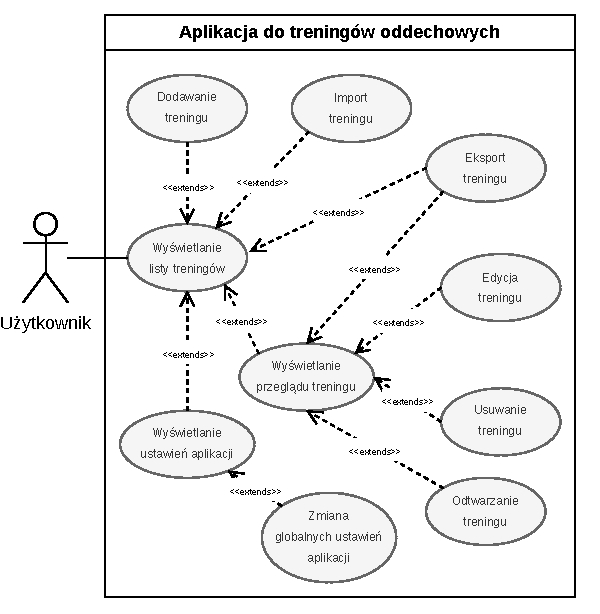
\includegraphics[width=0.90\linewidth,height=0.78\textheight,keepaspectratio]{obrazy/use_case.drawio-1.pdf}
    \caption{Diagram przypadków użycia aplikacji ReSpire}
    \label{fig:use_case_diagram}
\end{figure}

Jedynym aktorem przedstawionym na diagramie jest użytkownik aplikacji. Podstawowym przypadkiem użycia jest \textbf{Wyświetlanie listy treningów}, stanowiące główny punkt dostępu do pozostałych funkcji. Z tego miejsca użytkownik może wykonać przypadki: \textbf{Dodawanie treningu}, \textbf{Import treningu}, \textbf{Eksport treningu} albo \textbf{Wyświetlanie przeglądu treningu}. Zastosowane na diagramie relacje \textit{extend} wskazują działania opcjonalne, które rozszerzają podstawowy przebieg pracy z listą i są wykonywane dopiero po zgłoszeniu odpowiedniego żądania przez użytkownika.

\newpage

Przypadek \textbf{Dodawanie treningu} umożliwia zdefiniowanie jego nazwy, etapów, grup, liczby powtórzeń oraz parametrów poszczególnych faz oddechu. Po zatwierdzeniu poprawnie utworzony trening jest zapisywany i pojawia się na liście. \textbf{Import treningu} pozwala wczytać jeden lub kilka treningów z pliku o obsługiwanym formacie. Przed zapisem aplikacja powinna sprawdzić poprawność struktury danych, a w przypadku błędnego pliku przerwać operację i wyświetlić odpowiedni komunikat. \textbf{Eksport treningu} realizuje działanie odwrotne: dane treningu są przekształcane do postaci możliwej do zapisania i późniejszego ponownego zaimportowania.

Po wybraniu elementu z listy wykonywany jest przypadek \textbf{Wyświetlanie przeglądu treningu}. Ekran ten przedstawia jego strukturę, czasy faz, przyrosty oraz kolejność grup, dzięki czemu ustawienia mogą zostać sprawdzone przed rozpoczęciem ćwiczenia. Z poziomu przeglądu dostępne są trzy dalsze przypadki: \textbf{Edycja treningu}, \textbf{Usuwanie treningu} i \textbf{Odtwarzanie treningu}. Edycja pozwala zmienić istniejącą konfigurację i zapisać jej nową postać. Usuwanie wymaga potwierdzenia, ponieważ prowadzi do usunięcia treningu z lokalnych danych aplikacji. Odtwarzanie rozpoczyna sesję zgodnie z zapisanym wzorcem i uruchamia wybrane formy prowadzenia ćwiczenia, takie jak wizualizacja lub wskazówki dźwiękowe. Jeżeli monitorowanie za pomocą mikrofonu jest aktywne, podczas treningu może być również wykorzystywany moduł wykrywania wydechu.

Osobną grupę stanowią przypadki \textbf{Wyświetlanie ustawień aplikacji} i \textbf{Zmiana globalnych ustawień aplikacji}. Użytkownik może otworzyć widok ustawień i zmienić parametry obowiązujące globalnie, niezależnie od konfiguracji konkretnego treningu. Obejmują one między innymi sposób prezentowania ćwiczenia, zachowanie ekranu oraz ustawienia funkcji monitorujących. Oddzielenie ustawień globalnych od parametrów treningu ogranicza konieczność powtarzalnego konfigurowania tych samych opcji dla każdej sesji.

\section{Architektura rozwiązania}

System został podzielony na warstwę prezentacji, logikę aplikacji, moduł przetwarzania dźwięku oraz moduł wnioskowania. Taki podział ogranicza zależności pomiędzy interfejsem a modelem. Umożliwia również wymianę pliku ONNX bez przebudowy całej aplikacji oraz testowanie klasyfikatora niezależnie od warstwy wizualnej.

Warstwa Flutter odpowiada za interfejs i logikę aplikacji, natomiast uruchamianie modelu odbywa się w kodzie natywnym. Komunikacja pomiędzy kodem Dart a warstwami platformowymi jest realizowana za pomocą kanałów platformowych \cite{flutterPlatformChannels2026}. W zrealizowanej integracji BCV3 aplikacja przekazuje przygotowane dane wejściowe do modułu Kotlin w systemie Android. Kod natywny uruchamia model za pomocą ONNX Runtime, a następnie zwraca do Fluttera wynik detekcji wydechu. Warstwa aplikacyjna jest przygotowana również dla systemu iOS, jednak natywna integracja BCV3 w module Swift nie została przeprowadzona, przy czym pozostaje kierunkiem dalszych prac. Schemat architektury przedstawiono na rysunku \ref{fig:implementation_pipeline}; ścieżka dla iOS stanowi docelowy wariant integracji.

\begin{figure}[H]
    \centering
    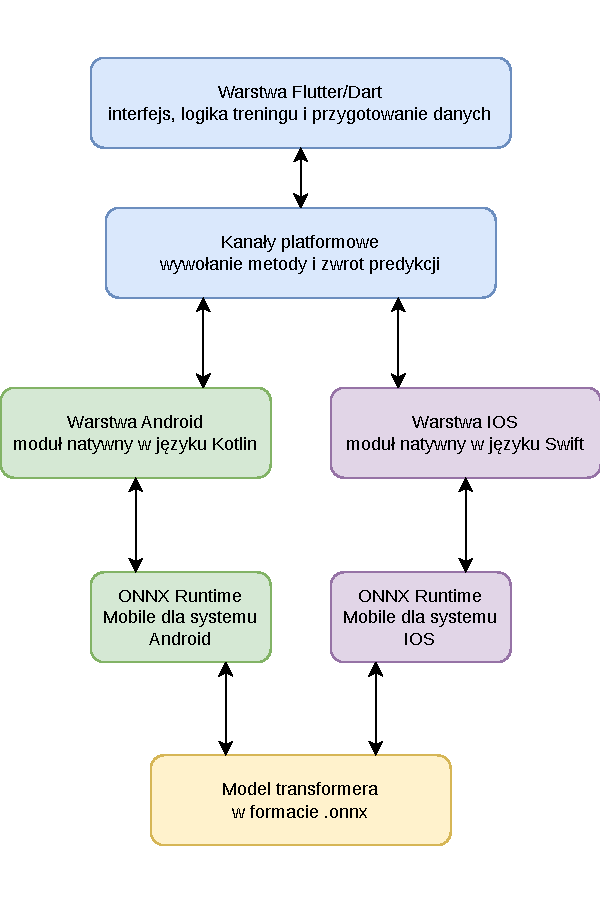
\includegraphics[width=0.82\linewidth,height=0.5\textheight,keepaspectratio]{obrazy/flow_diagram.pdf}
    \caption{Komunikacja warstwy Flutter z natywnymi modułami uruchamiającymi model ONNX}
    \label{fig:implementation_pipeline}
\end{figure}

Rozdzielenie etapu treningu i wnioskowania ma również znaczenie praktyczne. Proces uczenia może wykorzystywać komputer wyposażony w procesor graficzny, większą ilość pamięci oraz pełne środowisko PyTorch. Aplikacja końcowa zawiera wyłącznie model przeznaczony do predykcji i lekkie środowisko wykonawcze. Dzięki temu urządzenie mobilne nie musi udostępniać bibliotek używanych podczas trenowania.

\section{Warstwa aplikacyjna we Flutterze}

Do implementacji aplikacji wybrano Flutter, który umożliwia tworzenie interfejsu i logiki dla wielu platform z wykorzystaniem języka Dart oraz wspólnej bazy kodu \cite{flutterDocs2026}. Wybór tej technologii wynikał również z faktu, że wcześniejszy projekt ReSpire został już przygotowany we Flutterze. Kontynuowanie tej architektury ograniczyło koszt migracji, przy czym pozwoliło zachować istniejące komponenty.

Do rozwoju i testowania aplikacji mobilnej wykorzystano środowisko Android Studio. Zapewniało ono kompleksowe wsparcie dla kodu Flutter oraz Dart, jak i zarządzanie konfiguracją projektu dla systemu Android. Dzięki niemu możliwe było również uruchamianie aplikacji na emulatorze oraz podłączonym urządzeniu, a także analizowanie komunikatów diagnostycznych i błędów pojawiających się podczas działania aplikacji. Środowisko było również wykorzystywane podczas integracji warstwy Flutter z natywnym kodem Kotlin i biblioteką ONNX Runtime.

Warstwa Flutter odpowiada za uruchamianie sesji treningowej, obsługę uprawnień do mikrofonu, przechwytywanie danych, prezentację wyniku detekcji, a także sterowanie animacjami. Kod aplikacji został rozdzielony na elementy interfejsu, strony, usługi i funkcje pomocnicze. Komponenty wizualne mogą dzięki temu być modyfikowane niezależnie od kodu obsługującego dźwięk oraz model.

Z punktu widzenia interfejsu wynik modelu jest stanem aplikacji. Po otrzymaniu predykcji odpowiednie elementy ekranu są aktualizowane, aby wskazać wykrycie wydechu, który sygnalizuje koniec cyklu oddechowego. Ten sam wynik jest używany również do zliczania cykli i wyświetlenia odpowiedniej informacji o przebiegu treningu po jego zakończeniu. Interfejs nie musi znać szczegółów architektury sieci neuronowej, ponieważ otrzymuje jedynie etykietę oraz wartości wyjściowe modelu.

Wieloplatformowość Fluttera umożliwia utrzymywanie wspólnej logiki dla kolejnych systemów docelowych. Elementy zależne od platformy, takie jak konfiguracja uprawnień, sposób dostępu do mikrofonu lub integracja natywnego środowiska ONNX, mogą być wydzielone do odpowiednich katalogów platformowych albo obsłużone przez wtyczki. Pozwala to rozwijać wersje aplikacji bez duplikowania całej warstwy prezentacji.

\subsection{Diagram klas treningu}

Diagram klas przedstawia model danych wykorzystywany do zapisu konfiguracji treningu, ustawień sesji i przypisanych dźwięków. Pokazuje on zarówno hierarchię obiektów tworzących trening, jak i klasy pomocnicze odpowiedzialne za personalizację poszczególnych faz. Na diagramie wskazano również pliki źródłowe projektu, w których zawarto definicje poszczególnych klas. Aktualną postać modelu przedstawiono na rysunku \ref{fig:training_class_diagram}.

\begin{landscape}
\begin{figure}[H]
    \centering
    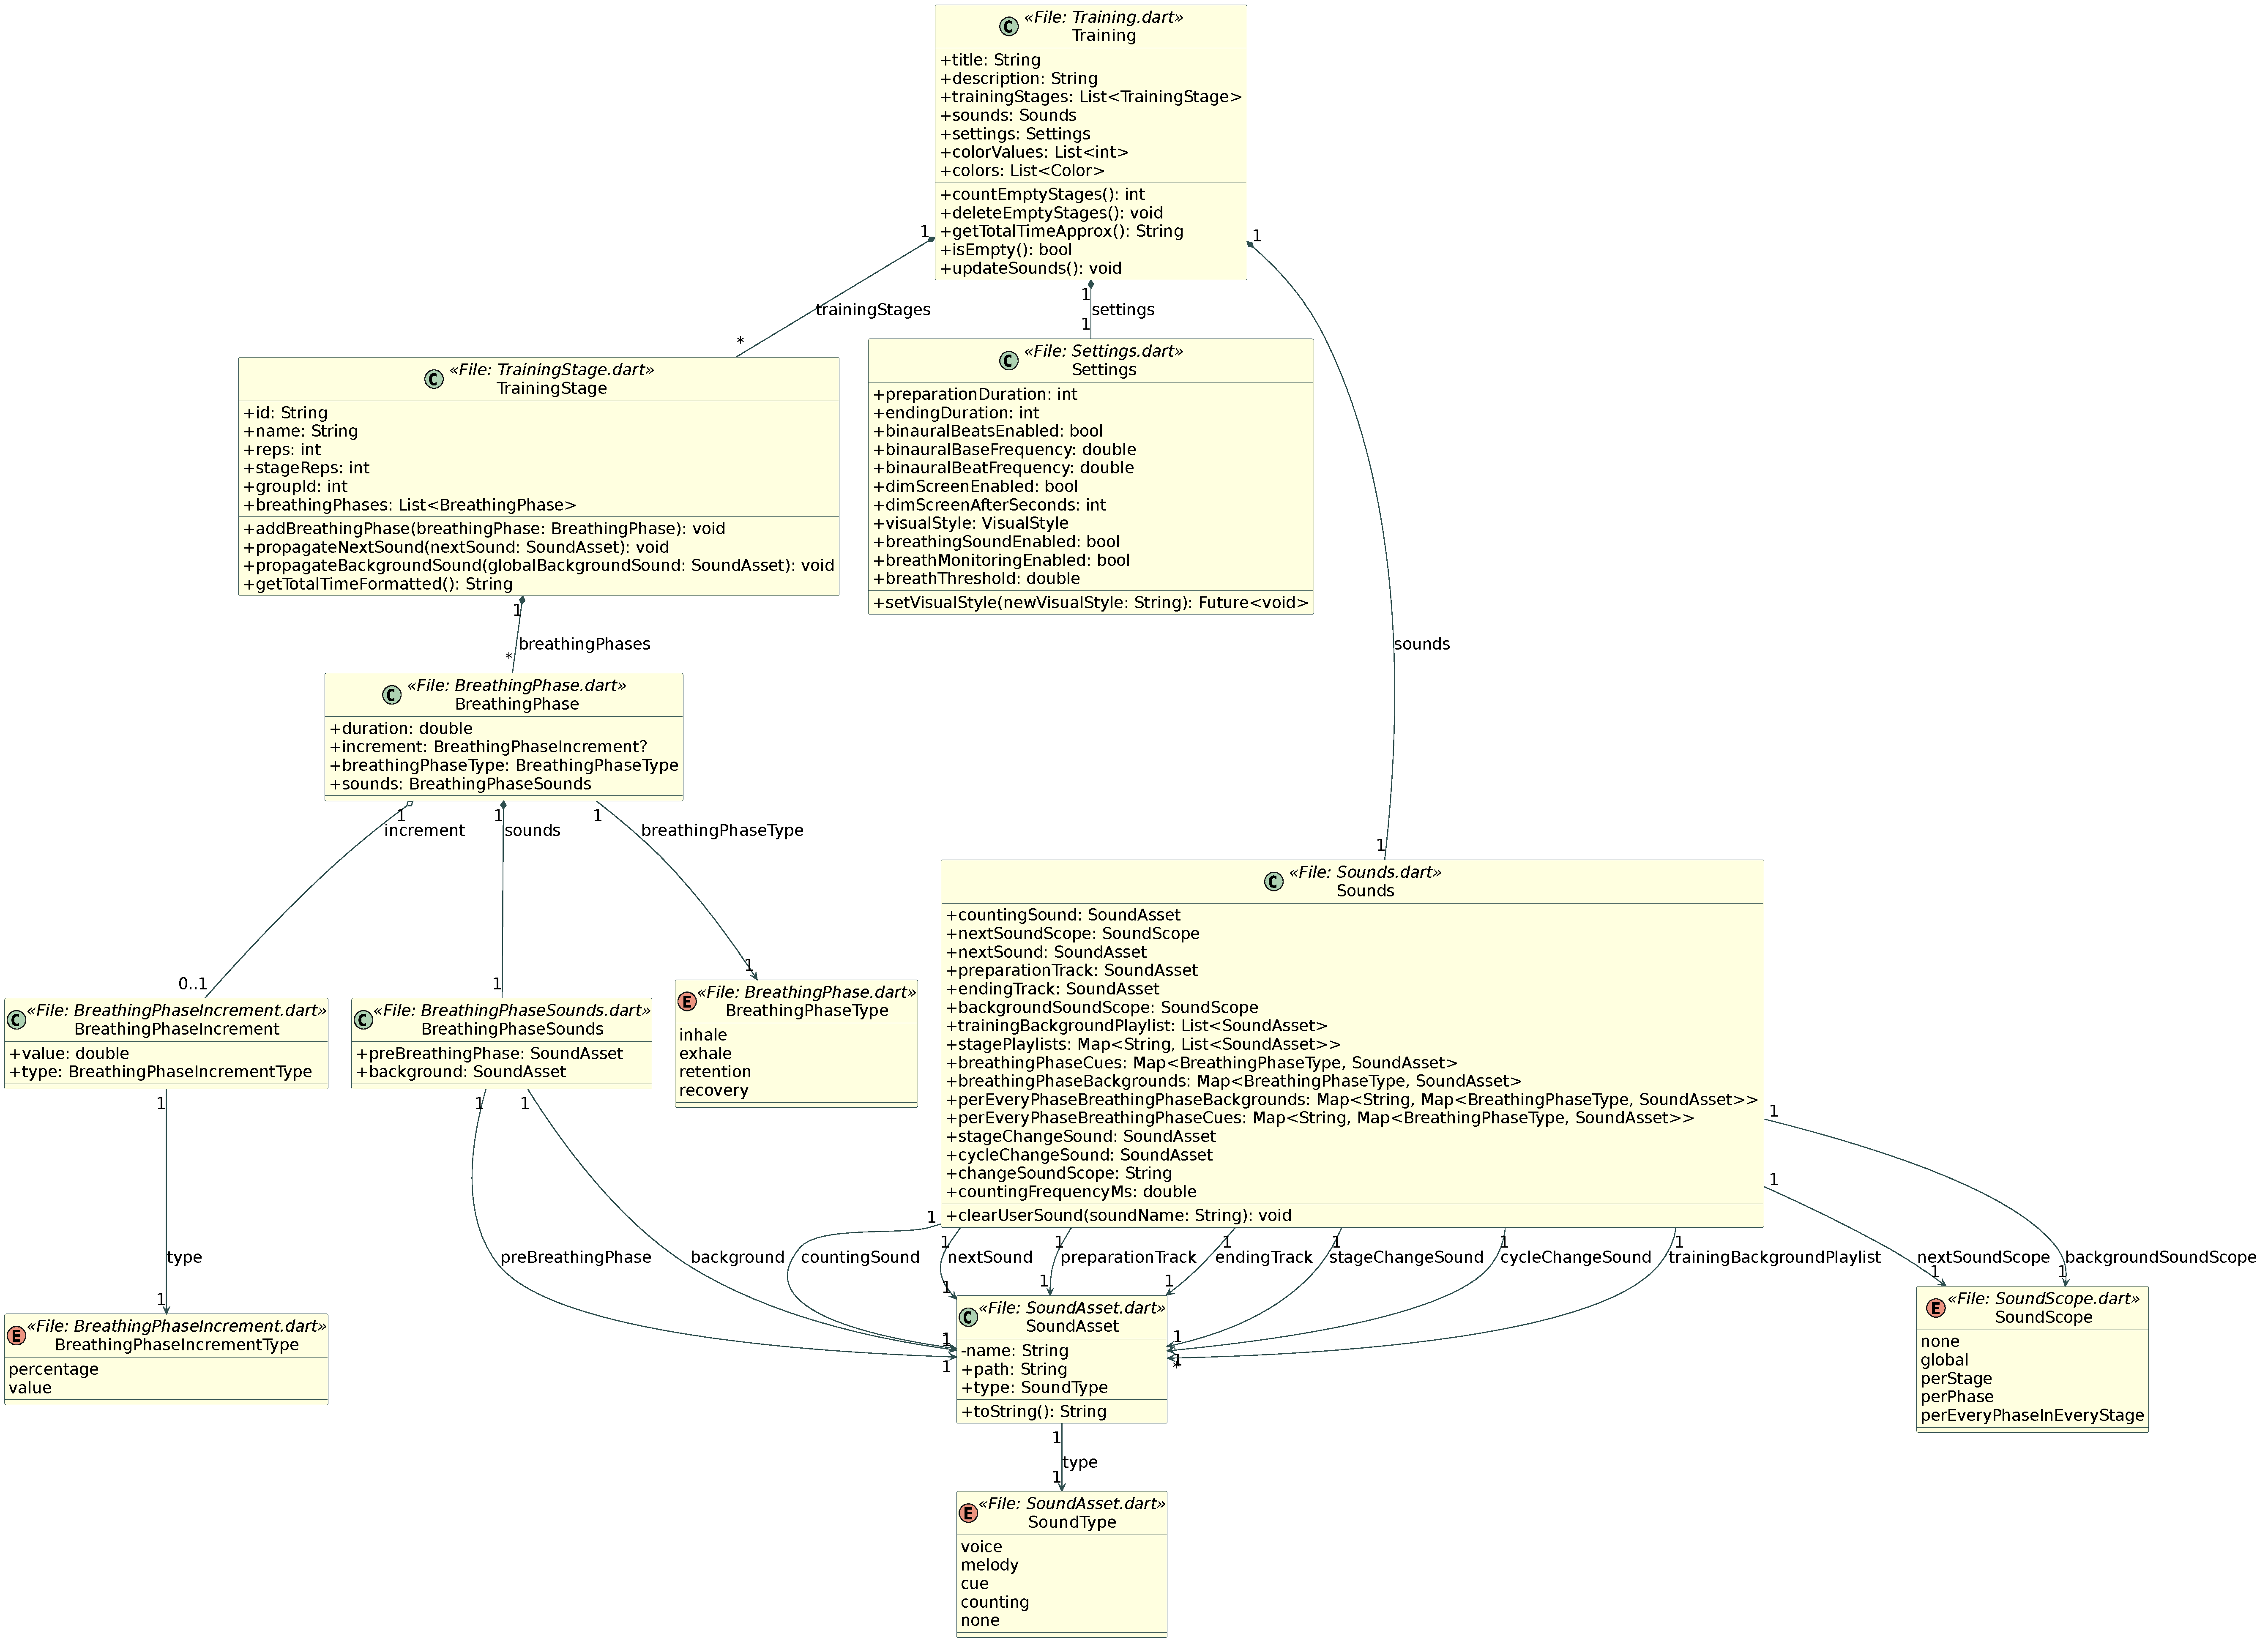
\includegraphics[width=\textheight,height=0.95\textwidth,keepaspectratio]{obrazy/use_case_files-1.pdf}
    \caption{Diagram klas modelu treningu aplikacji ReSpire}
    \label{fig:training_class_diagram}
\end{figure}
\end{landscape}

\subsection{Struktura danych treningu}

Model danych treningu ma strukturę hierarchiczną, której podstawę tworzą klasy \texttt{Training}, \texttt{TrainingStage}i \texttt{BreathingPhase}. Obiekt \texttt{Training} zawiera listę co najmniej jednego etapu, natomiast każdy etap składa się z uporządkowanej sekwencji faz \texttt{BreathingPhase}. Etapy mogą być dodatkowo łączone w grupy. Elementy należące do tej samej grupy są wykonywane kolejno, po czym cała grupa zostaje powtórzona zadaną liczbę razy. Dopiero po wykonaniu wszystkich powtórzeń aplikacja przechodzi do następnej grupy lub niezgrupowanego etapu.

Klasa \texttt{Training} przechowuje tytuł i opis treningu, listę etapów, ustawienia, konfigurację dźwięków oraz wartości kolorów wykorzystywane do wizualnego rozróżniania grup. Udostępnia również metody pomocnicze służące do wykrywania i usuwania pustych etapów, sprawdzania poprawności struktury, przybliżonego obliczania całkowitego czasu sesji oraz aktualizowania konfiguracji dźwiękowej. Pole \texttt{description} umożliwia uzupełnienie treningu o dodatkowy opis, natomiast \texttt{colorValues} i \texttt{colors} przechowują reprezentację kolorów w postaci możliwej do zapisania oraz obiekty wykorzystywane bezpośrednio przez interfejs.

Obiekt \texttt{TrainingStage} opisuje pojedynczy etap treningu. Oprócz identyfikatora, nazwy i listy faz zawiera pola \texttt{reps}, \texttt{stageReps} oraz \texttt{groupId}. Pole \texttt{reps} określa liczbę cykli wykonywanych wewnątrz etapu, natomiast \texttt{groupId} pozwala przypisać kilka etapów do wspólnej, uporządkowanej grupy. Pole \texttt{stageReps} określa liczbę powtórzeń całej grupy etapów. Klasa etapu nie przechowuje parametru przyrostu czasu, ponieważ progresja jest definiowana niezależnie dla każdej fazy oddechowej. \texttt{TrainingStage} umożliwia ponadto dodawanie faz, obliczanie łącznego czasu etapu oraz propagowanie dźwięku tła i sygnału kolejnej fazy do elementów podrzędnych.

Klasa \texttt{BreathingPhase} reprezentuje pojedynczą czynność oddechową. Pole \texttt{duration} określa jej podstawowy czas trwania, \texttt{breathingPhaseType} wskazuje rodzaj fazy, a \texttt{sounds} przechowuje jej oprawę dźwiękową. Typ wyliczeniowy \texttt{BreathingPhaseType} obejmuje wdech (\texttt{inhale}), wydech (\texttt{exhale}), zatrzymanie oddechu (\texttt{retention}) i regenerację (\texttt{recovery}). Każda faza może mieć własne, opcjonalne pole \texttt{increment}, dzięki czemu czas wdechu, wydechu, zatrzymania lub regeneracji może zmieniać się niezależnie w kolejnych cyklach.

Klasa \texttt{BreathingPhaseIncrement} odpowiada za zmianę czasu trwania konkretnej fazy wraz z kolejnymi powtórzeniami. Zawiera wartość \texttt{value} oraz sposób jej interpretacji określany przez \texttt{BreathingPhaseIncrementType}. Model obsługuje przyrost o wartość bezwzględną (\texttt{value}) oraz zmianę procentową (\texttt{percentage}). Pozwala to przykładowo stopniowo wydłużać wydech, nie zmieniając jednocześnie czasu pozostałych faz w tym samym etapie.

Globalne parametry sesji agreguje klasa \texttt{Settings}. Obejmuje ona czasy przygotowania i zakończenia, konfigurację dźwięków binauralnych, opcję wygaszania ekranu i czas bezczynności poprzedzający wygaszenie. Pole \texttt{visualStyle} wskazuje wybrany sposób wizualizacji treningu. Pola \texttt{breathingSoundEnabled}, \texttt{breathMonitoringEnabled} i \texttt{breathThreshold} sterują odpowiednio dźwiękowym prowadzeniem oddechu, działaniem modułu monitorowania oraz wartością progu detekcji. Metoda \texttt{setVisualStyle()} umożliwia aktualizację stylu wizualizacji wraz z zapisaniem zmiany.

Konfiguracja dźwięków została rozdzielona pomiędzy kilka powiązanych klas:

\begin{itemize}
    \item \texttt{Sounds} jest głównym kontenerem oprawy dźwiękowej treningu. Przechowuje dźwięk odliczania, utwory przygotowania oraz zakończenia, sygnały zmiany etapu i cyklu, globalną listę muzyki, a także listy przypisane do poszczególnych etapów. Mapy faz umożliwiają niezależne określenie sygnałów oraz dźwięków tła dla wdechu, wydechu, zatrzymania i regeneracji. Dodatkowe mapy indeksowane identyfikatorem etapu obsługują osobne ustawienia dla każdej fazy w każdej grupie. Pole \texttt{countingFrequencyMs} określa częstotliwość odtwarzania odliczania;
    \item \texttt{BreathingPhaseSounds} zawiera zasoby związane z pojedynczą fazą: sygnał \texttt{preBreathingPhase} odtwarzany przed jej rozpoczęciem oraz dźwięk \texttt{background} aktywny w czasie trwania fazy;
    \item \texttt{SoundAsset} reprezentuje pojedynczy zasób audio. Przechowuje jego nazwę, ścieżkę oraz kategorię wskazywaną przez \texttt{SoundType};
    \item \texttt{SoundType} rozróżnia głos lektora (\texttt{voice}), melodię (\texttt{melody}), krótki sygnał (\texttt{cue}), odliczanie (\texttt{counting}) i brak dźwięku (\texttt{none});
    \item \texttt{SoundScope} określa zakres obowiązywania dźwięku. Dostępne wartości oznaczają brak przypisania (\texttt{none}), ustawienie globalne (\texttt{global}), przypisanie do etapu (\texttt{perStage}), fazy (\texttt{perPhase}) albo każdej fazy w każdym etapie (\texttt{perEveryPhaseInEveryStage}).
\end{itemize}

Takie rozdzielenie odpowiedzialności pozwala zapisywać zarówno proste treningi wykorzystujące ustawienia globalne, jak i bardziej złożone sesje, w których każda grupa, etap lub faza ma własny czas, przyrost, kolor i oprawę dźwiękową. Jednocześnie dane pozostają możliwe do serializacji, co jest wykorzystywane podczas lokalnego zapisu oraz importu i eksportu treningów.

\subsection{Schemat bazy danych}

Schemat ERD przedstawia sposób zapisu modelu treningu w lokalnej bazie danych Hive. Głównym obiektem przechowywanym w kontenerze \texttt{respire} jest \texttt{Training}, który zawiera powiązane etapy, fazy oddechowe, ustawienia oraz konfigurację dźwięków. Na diagramie zaznaczono identyfikatory typów \texttt{HiveType}, numery pól \texttt{HiveField}, typy danych i pliki źródłowe zawierające definicje poszczególnych struktur. Widoczne relacje odpowiadają zagnieżdżeniu obiektów wykorzystywanemu podczas serializacji i odczytu treningu.

\begin{landscape}
\begin{figure}[H]
    \centering
    \makebox[\linewidth][c]{%
        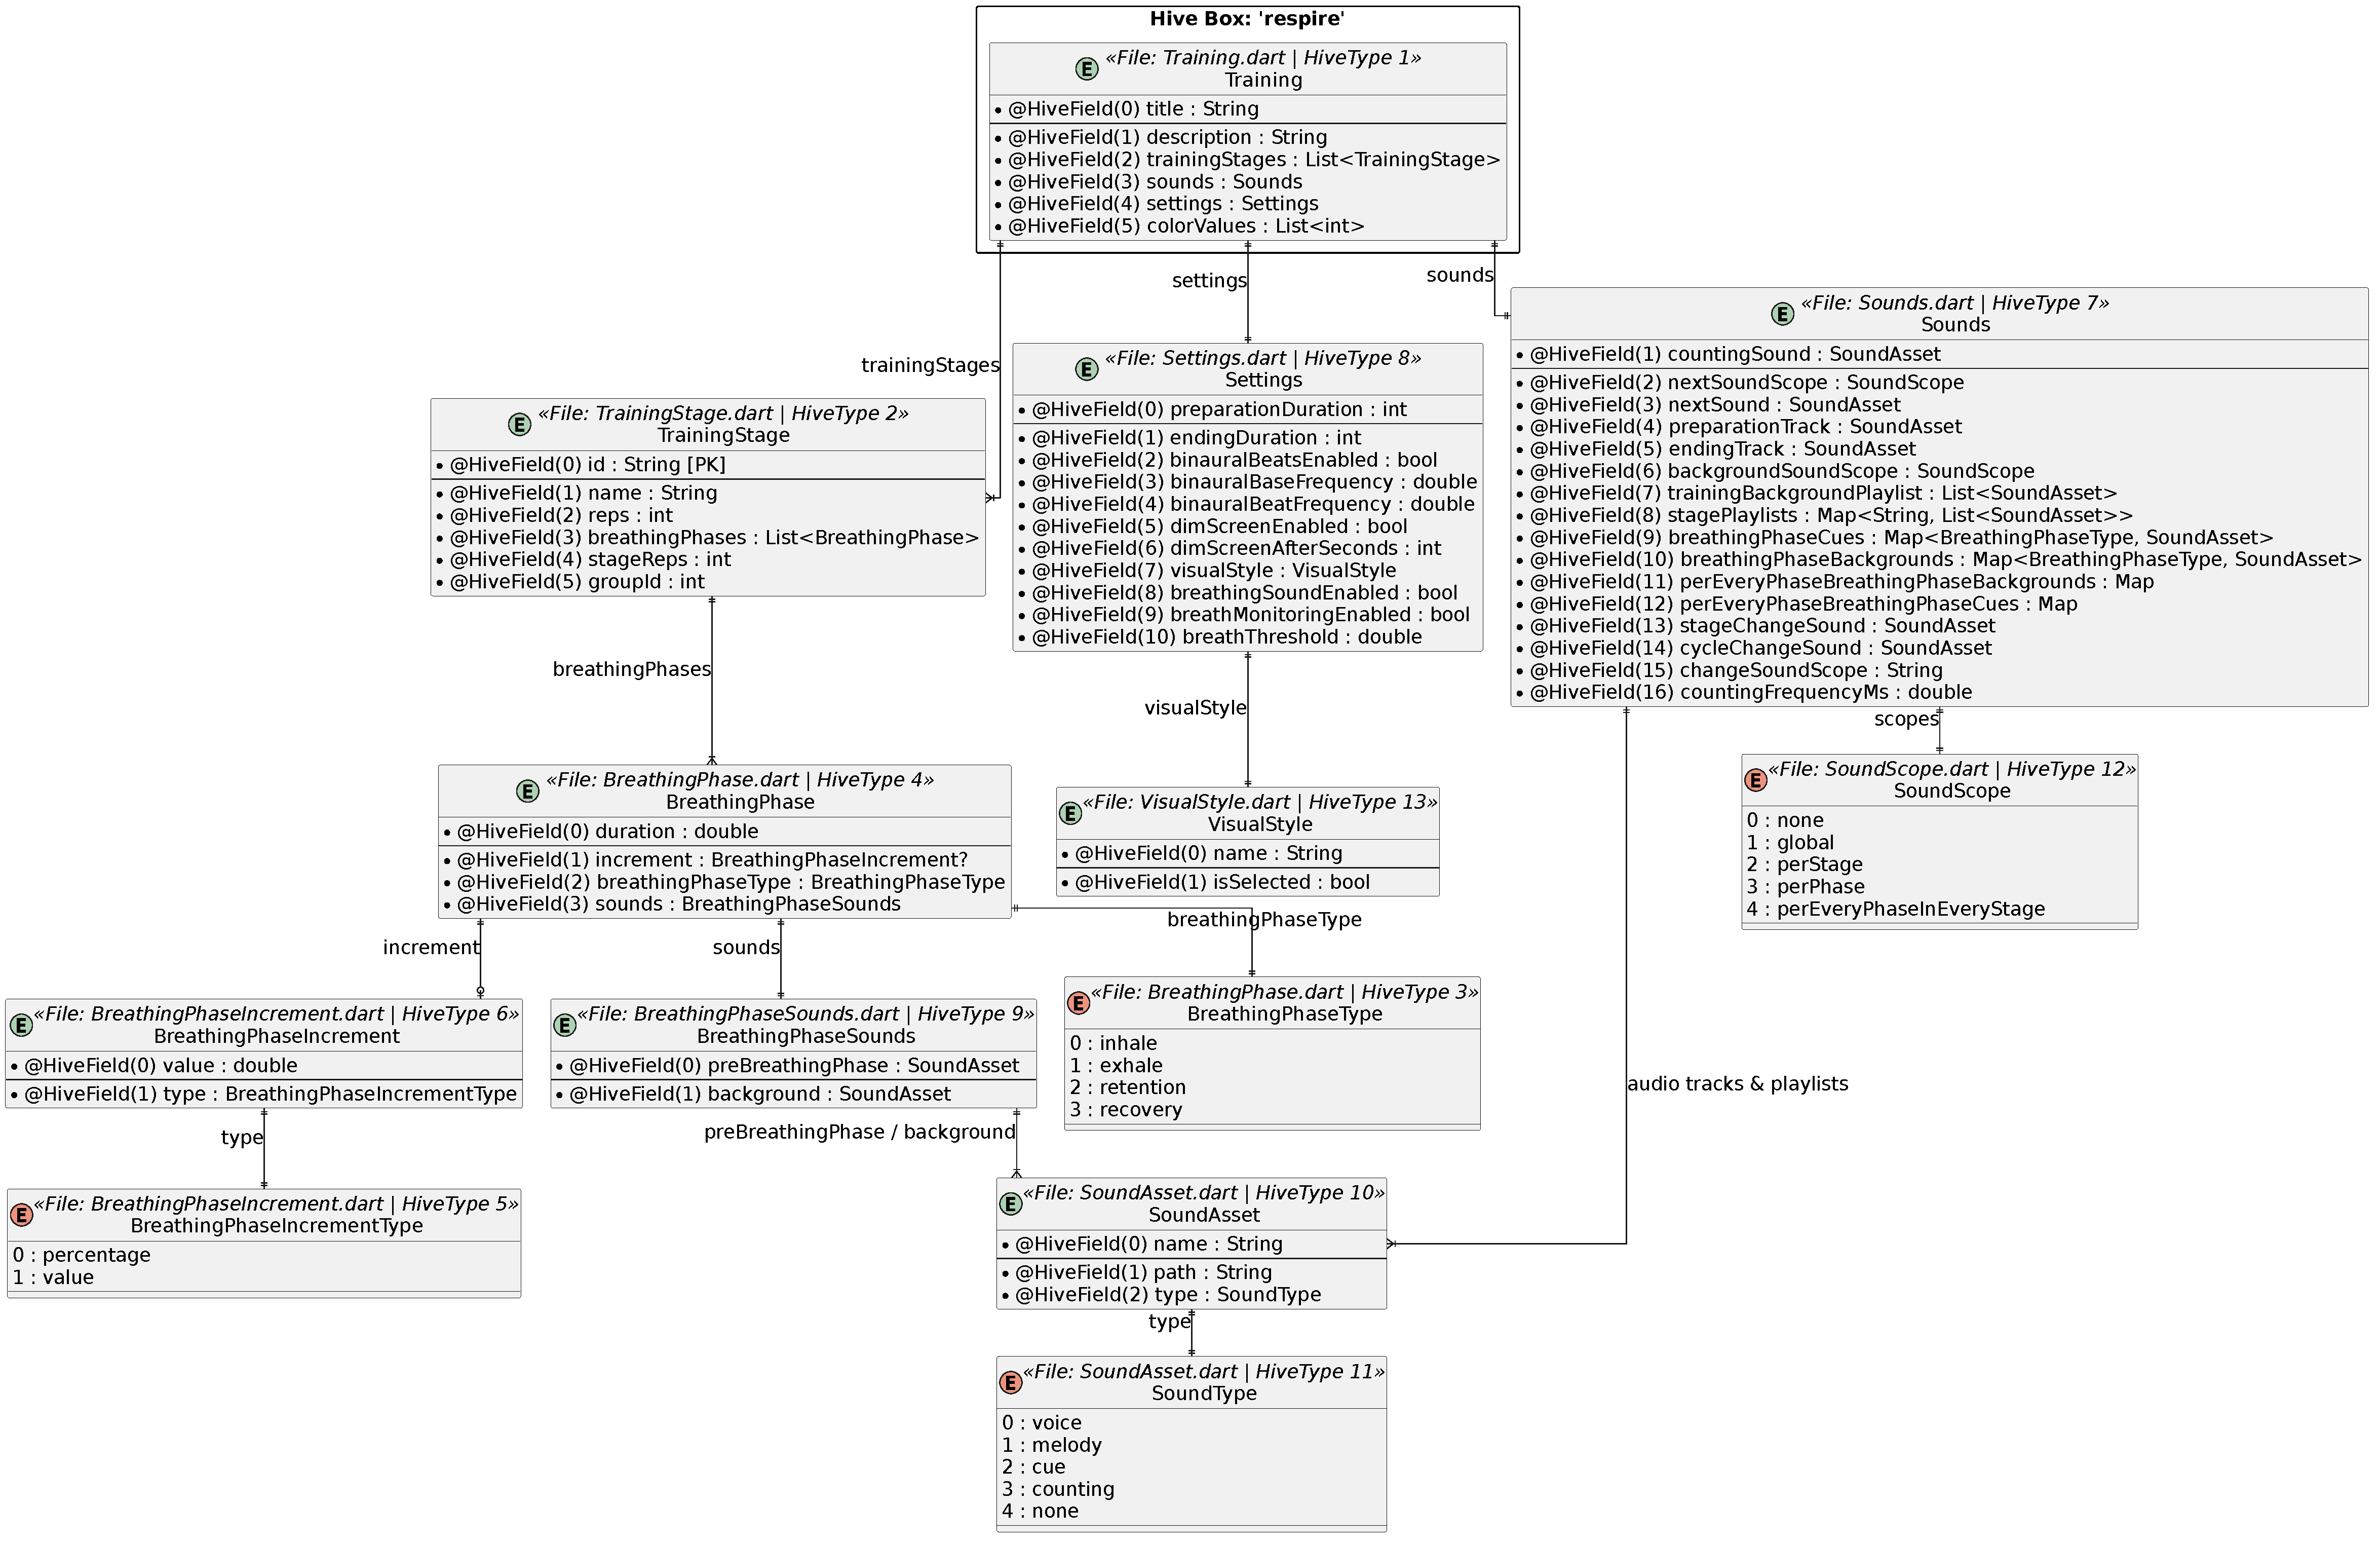
\includegraphics[width=1.10\textheight,height=1.05\textwidth,keepaspectratio]{obrazy/erd-1.pdf}%
    }
    \caption{Schemat ERD lokalnej bazy danych aplikacji ReSpire}
    \label{fig:training_erd}
\end{figure}
\end{landscape}

\subsection{Układ plików w repozytorium projektu aplikacji}

Repozytorium aplikacji składa się z części natywnej przeznaczonej dla systemu Android, katalogu zasobów oraz właściwego kodu aplikacji Flutter. Katalog \texttt{android} zawiera konfigurację projektu i pliki wymagane do zbudowania wersji mobilnej. Zasoby obejmują animacje, tłumaczenia, dźwięki i elementy graficzne, natomiast katalog \texttt{lib} przechowuje komponenty interfejsu, strony, usługi, motyw, funkcje pomocnicze oraz główny plik uruchamiający aplikację. Uproszczoną strukturę najważniejszych katalogów przedstawiono poniżej.

\dirtree{%
.1 android/.
.2 app/.
.3 src/.
.4 main/.
.3 build.gradle.
.2 gradle/.
.3 wrapper/.
.2 build.gradle.
.2 gradle.properties.
.2 settings.gradle.
.1 android/app/src/main/assets/.
.2 animations/.
.3 wave.json.
.2 languages/.
.3 en-US.json.
.3 pl-PL.json.
.2 sounds/.
.3 generator.dart.
.2 group\_logo.png.
.2 logo\_bez\_tla.png.
.1 lib/.
.2 components/.
.3 BreathingPage/.
.3 Global/.
.3 HomePage/.
.3 Settings/.
.3 TrainingEditorPage/.
.2 pages/.
.3 BreathingPage.dart.
.3 HomePage.dart.
.3 ProfilePage.dart.
.3 SettingsPage.dart.
.3 TrainingEditorPage.dart.
.3 TrainingPage.dart.
.2 services/.
.3 SoundManagers/.
.3 TranslationProvider/.
.3 BinauralBeatGenerator.dart.
.3 SettingsProvider.dart.
.3 TrainingController.dart.
.3 TrainingImportExportService.dart.
.3 UserSoundsDataBase.dart.
.2 theme/.
.3 Colors.dart.
.2 utils/.
.3 DurationFormatter.dart.
.3 TextUtils.dart.
.2 main.dart.
}

\section{Model CNN-Transformer w PyTorch}

Model klasyfikujący został zaimplementowany w PyTorch \cite{pytorchDocs2026}. Bibliotekę tę wybrano jako nowoczesne rozwiązanie zapewniające swobodę implementacji i intuicyjny sposób definiowania modeli, a także dostępność gotowych elementów transformera oraz możliwość przeprowadzenia treningu, ewaluacji i eksportu w jednym środowisku.

Do rozwoju kodu modelu w języku Python, uruchamiania skryptów treningowych, jak również analizy wyników wykorzystano środowisko Visual Studio Code.

Wejściem modelu nie jest bezpośrednio pełne nagranie, lecz krótki fragment dźwięku przekształcony do spektrogramu mel. Zgodnie z konfiguracją udokumentowaną w repozytorium modelu wykorzystywana jest częstotliwość próbkowania 44,1 kHz, okna o długości 0,3 s oraz reprezentacja zawierająca 128 pasm mel \cite{breathingClassificationGithub2026}. Takie podejście zapewnia krótki czas reakcji i umożliwia bieżące wykrywanie wydechu podczas treningu.

Zastosowany model bazowy ma architekturę hybrydową CNN-Transformer. Spektrogram mel jest najpierw przetwarzany przez ekstraktor cech złożony z trzech warstw splotowych Conv2D oraz operacji redukujących wymiar częstotliwościowy. Uzyskane mapy cech są spłaszczane do sekwencji ramek czasowo-częstotliwościowych, rzutowane liniowo do wymiaru modelu i uzupełniane kodowaniem pozycyjnym. Tak przygotowana sekwencja trafia do enkodera transformera, po którym zastosowano warstwę dropout oraz w pełni połączoną głowicę wyjściową generującą predykcje dla kolejnych ramek. W aplikacji wynik modelu jest wykorzystywany wyłącznie do wykrywania wydechu. Podczas działania aplikacji rozpoznany wydech oznacza zakończenie cyklu oddechowego, a także stanowi podstawę do zwiększenia licznika.

Do aplikacji Flutter dołączany jest gotowy, wcześniej wytrenowany model zapisany w formacie ONNX. Podczas działania aplikacji jego architektura i wyuczone wagi nie są modyfikowane. Zmiana sposobu działania modelu wymaga przeprowadzenia ponownego treningu w środowisku Python, ponownego eksportu oraz zastąpienia pliku ONNX w zasobach aplikacji. Bez ponownego uczenia można regulować jedynie próg decyzyjny, na podstawie którego wynik modelu jest uznawany za wykrycie wydechu. Zmiana progu wpływa na czułość detekcji, która może wymagać dostosowania w zależności od używanego sprzętu.

\section{Eksport modelu do ONNX}

Model utworzony w PyTorch nie jest bezpośrednio dołączany do aplikacji. Po zakończeniu treningu jest przełączany w tryb ewaluacji i eksportowany do formatu ONNX. PyTorch udostępnia w tym celu moduł \texttt{torch.onnx}, który przekształca graf obliczeniowy do przenośnej reprezentacji \cite{pytorchOnnxExporter2026}. W katalogu modelu transformerowego służy do tego osobny skrypt \texttt{export\_to\_onnx.py} \cite{breathingClassificationGithub2026}.

ONNX pełni funkcję warstwy pośredniej pomiędzy środowiskiem treningowym a aplikacją. Format zapisuje strukturę grafu, operatory oraz parametry modelu, dzięki czemu wnioskowanie nie wymaga uruchamiania interpretera Pythona ani pełnego PyTorch \cite{onnxConcepts2026}. Plik jest umieszczany w~zasobach aplikacji, a następnie otwierany przez warstwę wykonawczą zgodną z ONNX Runtime. Środowisko to obsługuje wykonywanie modeli między innymi na systemie Android lub iOS \cite{onnxRuntimeMobile2026}.

Podczas integracji należy zachować zgodność wejścia modelu z przetwarzaniem zastosowanym w Pythonie. Dotyczy to częstotliwości próbkowania, długości okna, liczby pasm mel, kolejności wymiarów tensora, typu danych oraz normalizacji. Należy przy tym zachować szczególną ostrożność, ponieważ nawet poprawnie wyeksportowany model może zwracać błędne wyniki, jeżeli aplikacja przygotuje spektrogram w inny sposób niż kod użyty podczas treningu.

Weryfikacja eksportu polega na przekazaniu tych samych danych wejściowych do wersji PyTorch i ONNX, jak również porównaniu uzyskanych wartości. Różnice powinny mieścić się w tolerancji wynikającej z obliczeń zmiennoprzecinkowych. Następnie model jest testowany w pełnym potoku aplikacji, obejmującym pobranie dźwięku, przygotowanie cech, wnioskowanie oraz aktualizację interfejsu.

\section{Działanie aplikacji}

Po uruchomieniu treningu aplikacja uzyskuje dostęp do mikrofonu i rozpoczyna odbieranie próbek audio. Dane są gromadzone do momentu utworzenia okna o wymaganej długości. Następnie wykonywane jest przetwarzanie wstępne, a także obliczenie reprezentacji wejściowej. Tensor trafia do modelu ONNX, który zwraca wynik określający obecność wydechu w analizowanym fragmencie. Pełny przepływ przetwarzania sygnału, od pozyskania dźwięku do wyświetlenia informacji zwrotnej w interfejsie użytkownika, przedstawiono na rysunku \ref{fig:breath_flow_chart}.

\begin{figure}[H]
    \centering
    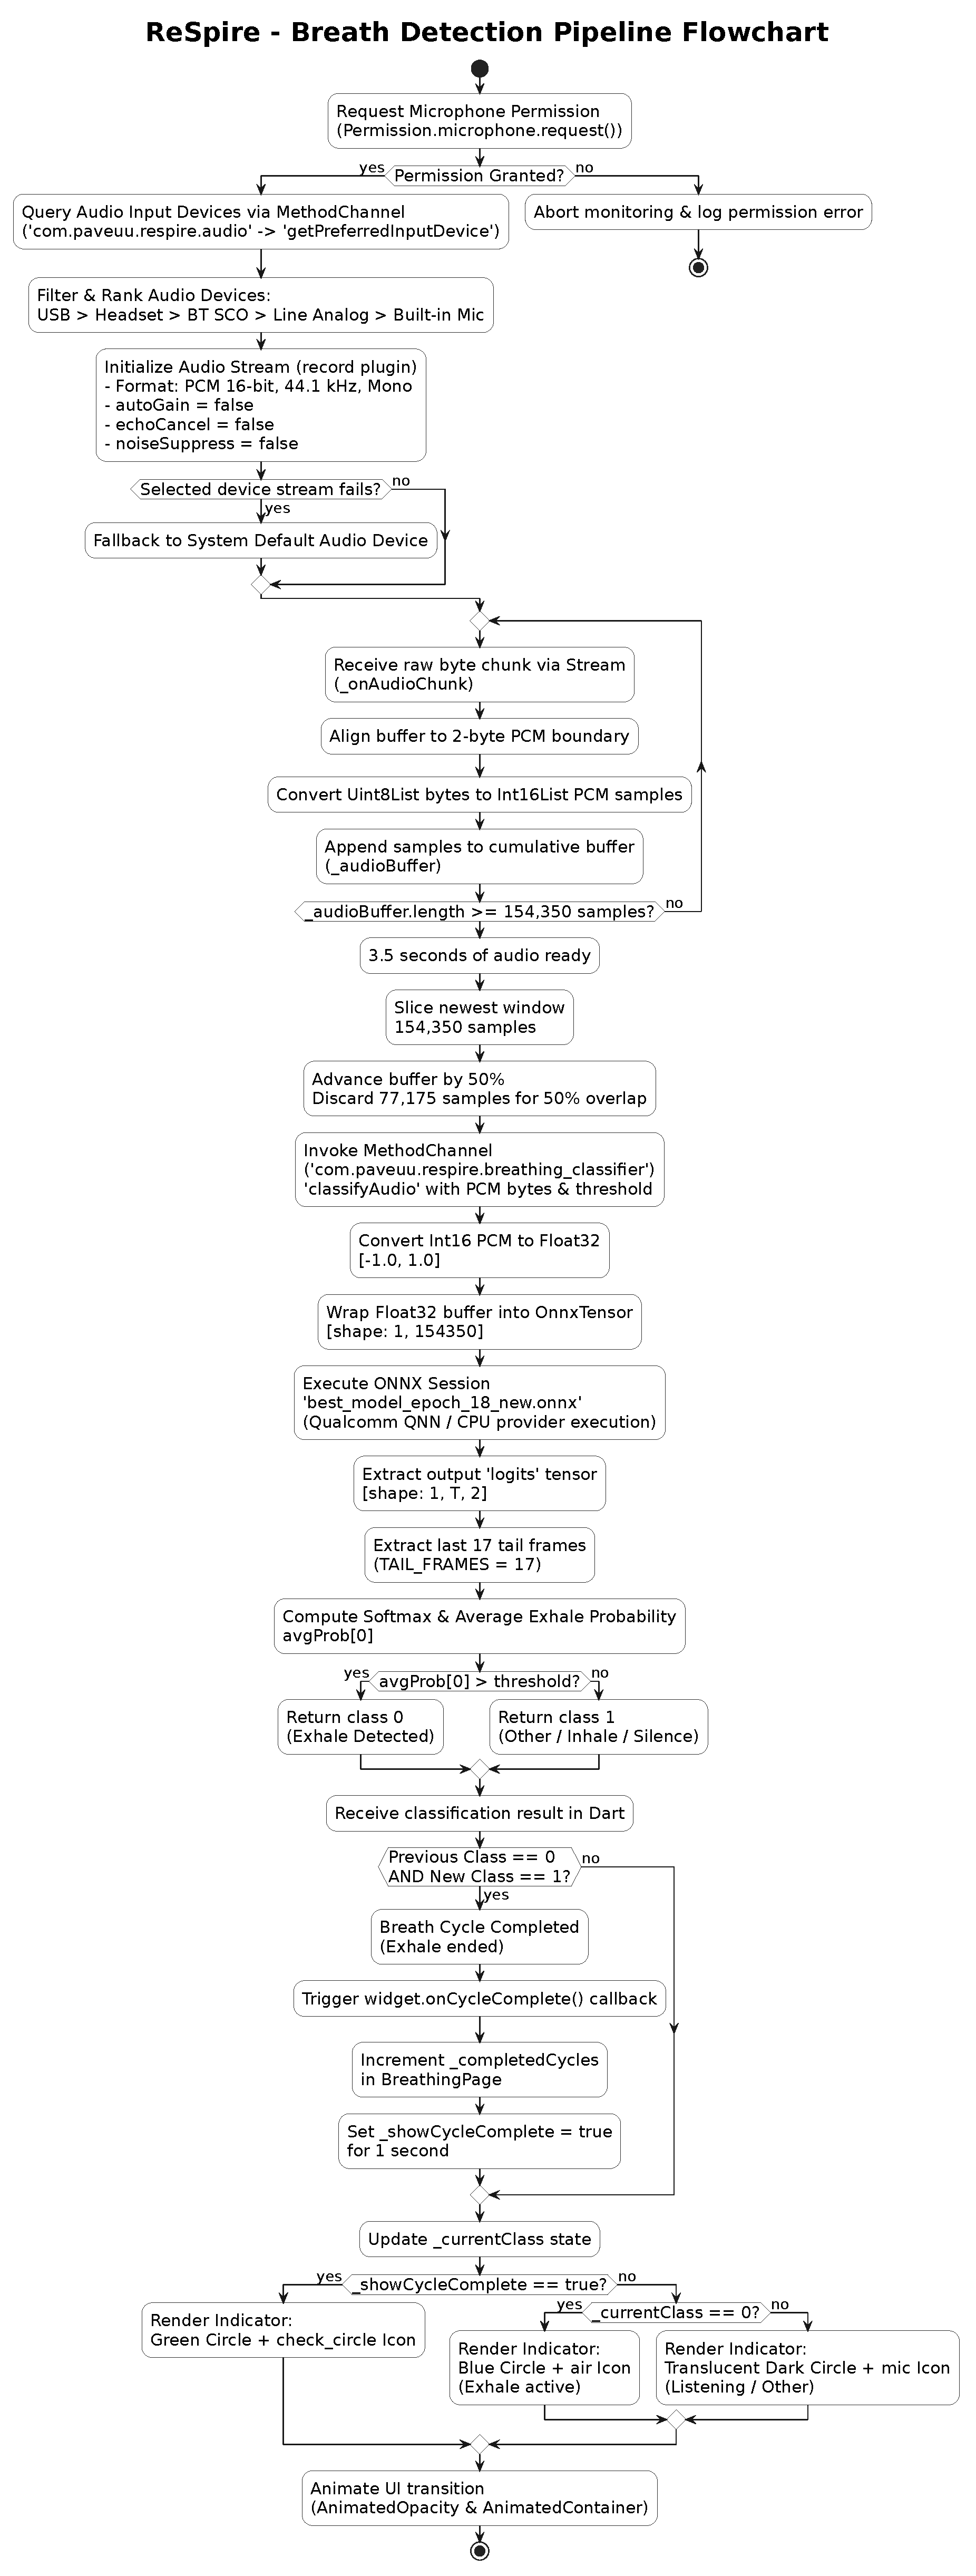
\includegraphics[width=0.95\linewidth,height=0.72\textheight,keepaspectratio]{obrazy/breath_flow_chart.pdf}
    \caption{Przepływ przetwarzania sygnału oddechowego od jego pozyskania do wyświetlenia informacji zwrotnej w interfejsie użytkownika}
    \label{fig:breath_flow_chart}
\end{figure}

Wynik detekcji jest przekazywany do interfejsu aplikacji. Rozpoznanie wydechu oznacza zakończenie bieżącego cyklu oddechowego i powoduje zwiększenie jego licznika. Proces jest powtarzany dla kolejnych fragmentów nagrania, dzięki czemu aplikacja może na bieżąco monitorować przebieg treningu. Implementacja modelu nie służy do pełnej klasyfikacji faz oddechu, lecz wyłącznie do identyfikowania wydechów potrzebnych do zliczania cykli.

Gdy model nie wykryje wydechu, licznik pozostaje bez zmian. Pozwala to pominąć wdechy, przerwy w treningu oraz fragmenty, które nie zawierają cech charakterystycznych dla wydechu.

\section{Iteracyjny proces rozwoju i dokumentacja}

Projekt był rozwijany iteracyjnie, a kolejne wersje kodu zapisywano w repozytorium GitHub. Każda większa zmiana mogła być analizowana jako osobny etap rozwoju: od modyfikacji interfejsu ReSpire, przez integrację modułu \texttt{exhale\_detection}, po zastosowanie transformera i eksport ONNX. Historia zmian umożliwiała porównywanie wariantów, odtwarzanie wcześniejszych wersji oraz wskazanie momentu wprowadzenia poszczególnych funkcji.

Projekt był rozwijany w dwóch oddzielnych repozytoriach, odpowiadających jego głównym warstwom. Repozytorium \textit{ReSpire} zawierało aplikację mobilną. Drugie repozytorium, \textit{breathing-classification-v3} obejmowało część związaną ze sztuczną inteligencją. Zawierało ono kod związany z  przygotowaniem i przetwarzaniem danych, implementację oraz trening modelu, jego ewaluację, jak również eksport do formatu ONNX. Rozdzielenie obu części umożliwiało niezależne rozwijanie aplikacji i modelu, przy zachowaniu jasno określonego sposobu ich integracji. Pozwoliło to zachować czytelność oraz porządek obu części.

\subsection{Zarządzanie zadaniami w Trello}

Do planowania prac i śledzenia postępu wykorzystano również narzędzie Trello. Tablica projektu stanowiła uzupełnienie systemu kontroli wersji. Umożliwiła ona organizowanie zadań związanych z rozwojem aplikacji. Poszczególne listy odpowiadały kolejnym wersjom systemu, a~umieszczone na nich karty opisywały planowane funkcje, poprawki interfejsu, zadania techniczne oraz wykryte problemy.

Taki sposób organizacji ułatwiał określenie zakresu kolejnych iteracji, a także kontrolowanie stopnia realizacji poszczególnych zmian. Po ukończeniu zadania jego stan był aktualizowany na tablicy, dzięki czemu możliwe było szybkie sprawdzenie, które elementy danej wersji zostały wykonane, a~które wymagały dalszej pracy. Ukończenie każdej owej listy było finalizowane zbudowaniem nowej wersji aplikacji. Przykładową postać tablicy wykorzystywanej podczas rozwoju aplikacji przedstawiono na rysunku \ref{fig:trello_board}.

\begin{figure}[H]
    \centering
    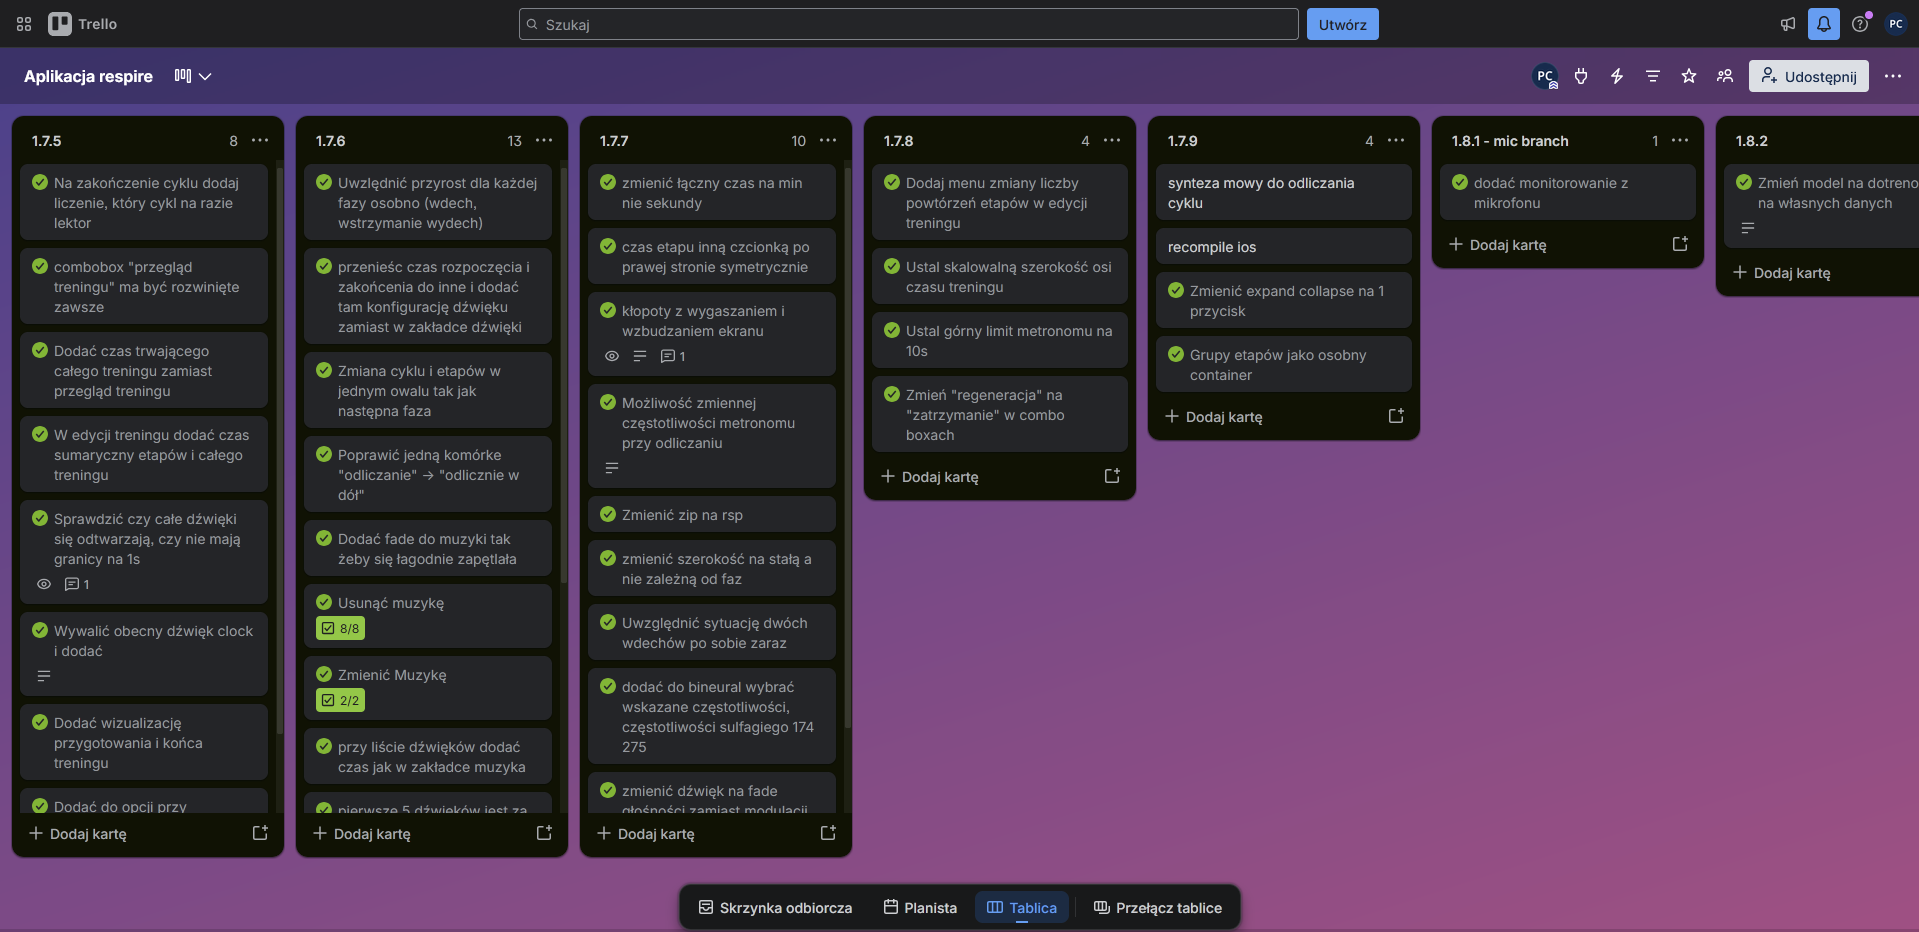
\includegraphics[width=\linewidth,height=0.72\textheight,keepaspectratio]{obrazy/trello-board.png}
    \caption{Tablica Trello wykorzystywana do zarządzania zadaniami i kolejnymi wersjami aplikacji}
    \label{fig:trello_board}
\end{figure}

\section{Podsumowanie}

Zaimplementowane rozwiązanie łączy wieloplatformową aplikację Flutter z modelem CNN-Transformer przygotowanym w PyTorch. Format ONNX oddziela środowisko treningowe od mobilnego środowiska wykonawczego i umożliwia integrację modelu bez osadzania Pythona w aplikacji. ReSpire dostarczył podstawę interfejsu. Projekt klasyfikacji oddechu, jak również moduł detekcji wydechu zapewniły natomiast punkt wyjścia dla analizy dźwięku oraz zliczania cykli na podstawie wykrytych wydechów.

Iteracyjny rozwój w repozytoriach GitHub umożliwił stopniowe udoskonalanie interfejsu, modelu i sposobu ich integracji. Przyjęta architektura pozostawia możliwość dalszego rozwijania każdej warstwy niezależnie, np. zastąpienia modelu nowszą wersją ONNX, dodania kolejnej platformy docelowej lub rozszerzenia aplikacji o historię treningów, a także dodatkowe formy wizualizacji.
\chapter{Eksperymenty i wyniki}

W rozdziale przedstawiono zmiany interfejsu i funkcjonalności aplikacji wprowadzone w celu poprawy doświadczenia użytkownika oraz wyniki badań modelu wykrywania wydechu. Porównano ekrany przed modyfikacjami, a także po ich wdrożeniu, a następnie przeanalizowano skuteczność modeli BCV2 i BCV3 oraz dobór progu decyzyjnego w różnych konfiguracjach sprzętowych.

\section{Badania związane z UX/UI}

Prace nad interfejsem obejmowały przegląd treningu, sposób prezentowania ćwiczeń, edycję etapów, ustawienia dźwięku i konfigurację detekcji wydechu. Celem zmian było zwiększenie czytelności ekranów oraz rozszerzenie możliwości dostosowania treningu do preferencji użytkownika. Poniższe zestawienia dokumentują zakres wprowadzonych usprawnień. Mają charakter porównania funkcjonalnego, jak również wizualnego.

\subsection{Usprawnienie ekranu przeglądu treningu}

Ekran przeglądu treningu rozszerzono o prezentację podziału etapów na grupy. Użytkownik może przed rozpoczęciem ćwiczenia sprawdzić kolejność grup, należące do nich etapy oraz liczbę powtórzeń. Wyróżnienie grup kolorami ułatwia odczytanie struktury treningu, zwłaszcza gdy obejmuje on kilka różnych sekwencji oddechowych.


Dodatkowo przyrost czasu trwania jest przedstawiany osobno dla każdej fazy, gdzie w poprzednich wersjach nie był on wyświetlany w ogóle. Sposób prezentacji wynika z wprowadzonej w edytorze treningu możliwości niezależnego dostosowywania przyrostu dla poszczególnych faz. Widoczne wartości odzwierciedlają ustawienia wybrane podczas edycji i pozwalają użytkownikowi sprawdzić je przed rozpoczęciem ćwiczenia. Porównanie obu wersji ekranu przedstawiono na rysunku \ref{fig:ux_training_overview}.

\begin{figure}[H]
    \centering
    \begin{minipage}[c]{0.44\linewidth}
        \centering
        {\setlength{\fboxsep}{0pt}\setlength{\fboxrule}{0.2pt}\fcolorbox{gray}{white}{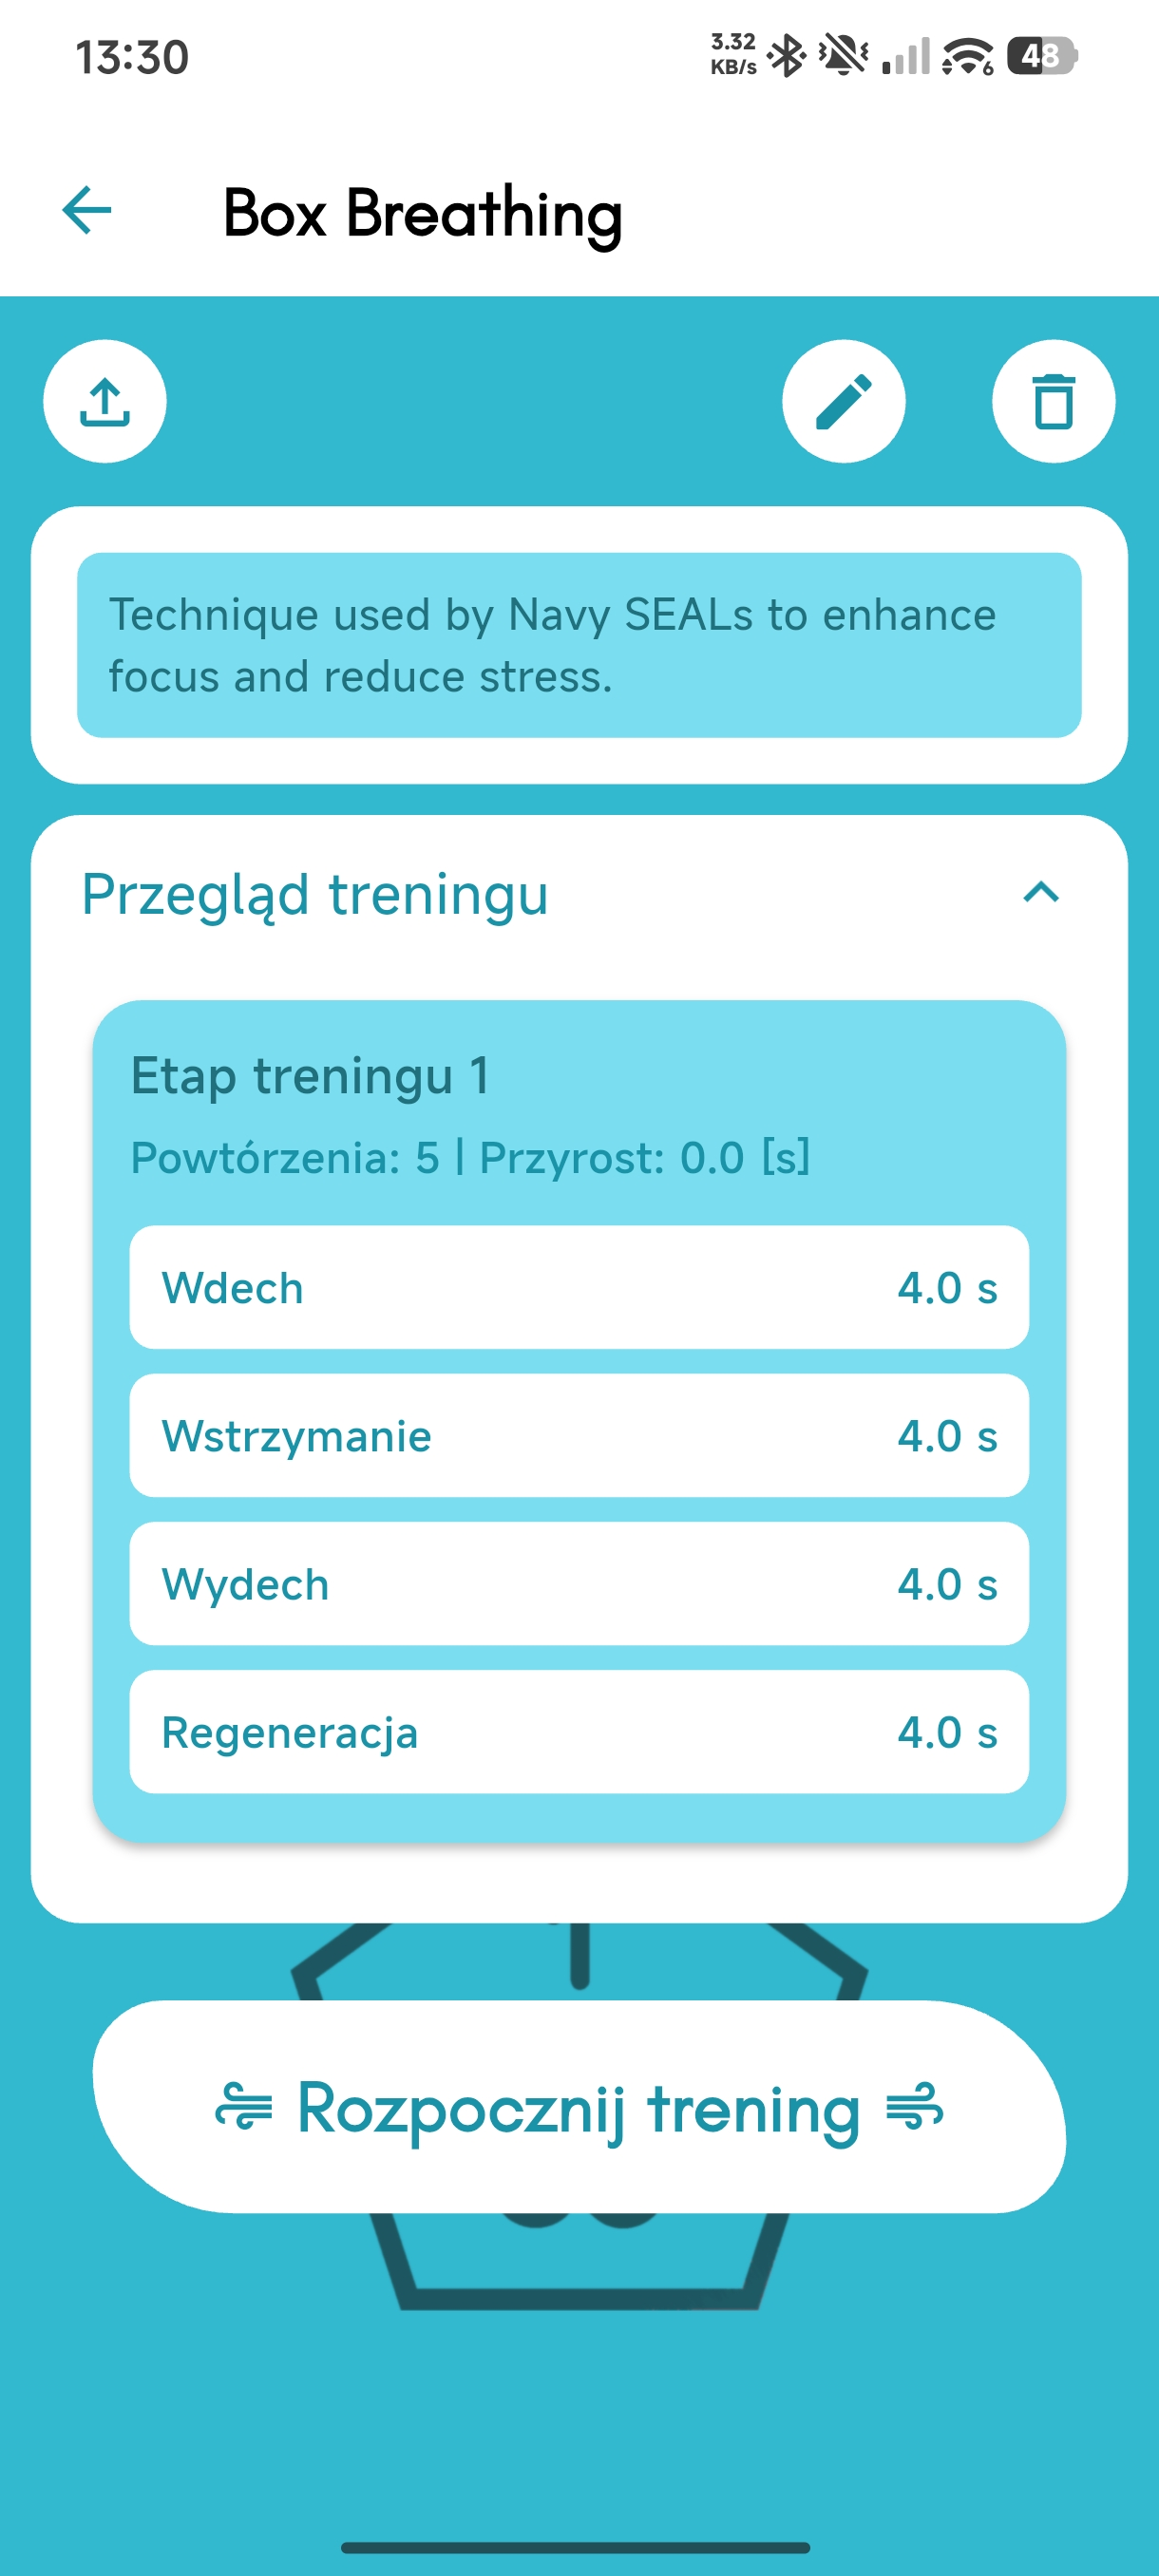
\includegraphics[width=\dimexpr\linewidth-2\fboxrule\relax,height=0.64\textheight,keepaspectratio]{obrazy/badania_interface/start_menu_old.jpg}}}
        \par\small (a)
    \end{minipage}\hfill
    \begin{minipage}[c]{0.08\linewidth}
        \centering
        {\large $\rightarrow$}
    \end{minipage}\hfill
    \begin{minipage}[c]{0.44\linewidth}
        \centering
        {\setlength{\fboxsep}{0pt}\setlength{\fboxrule}{0.2pt}\fcolorbox{gray}{white}{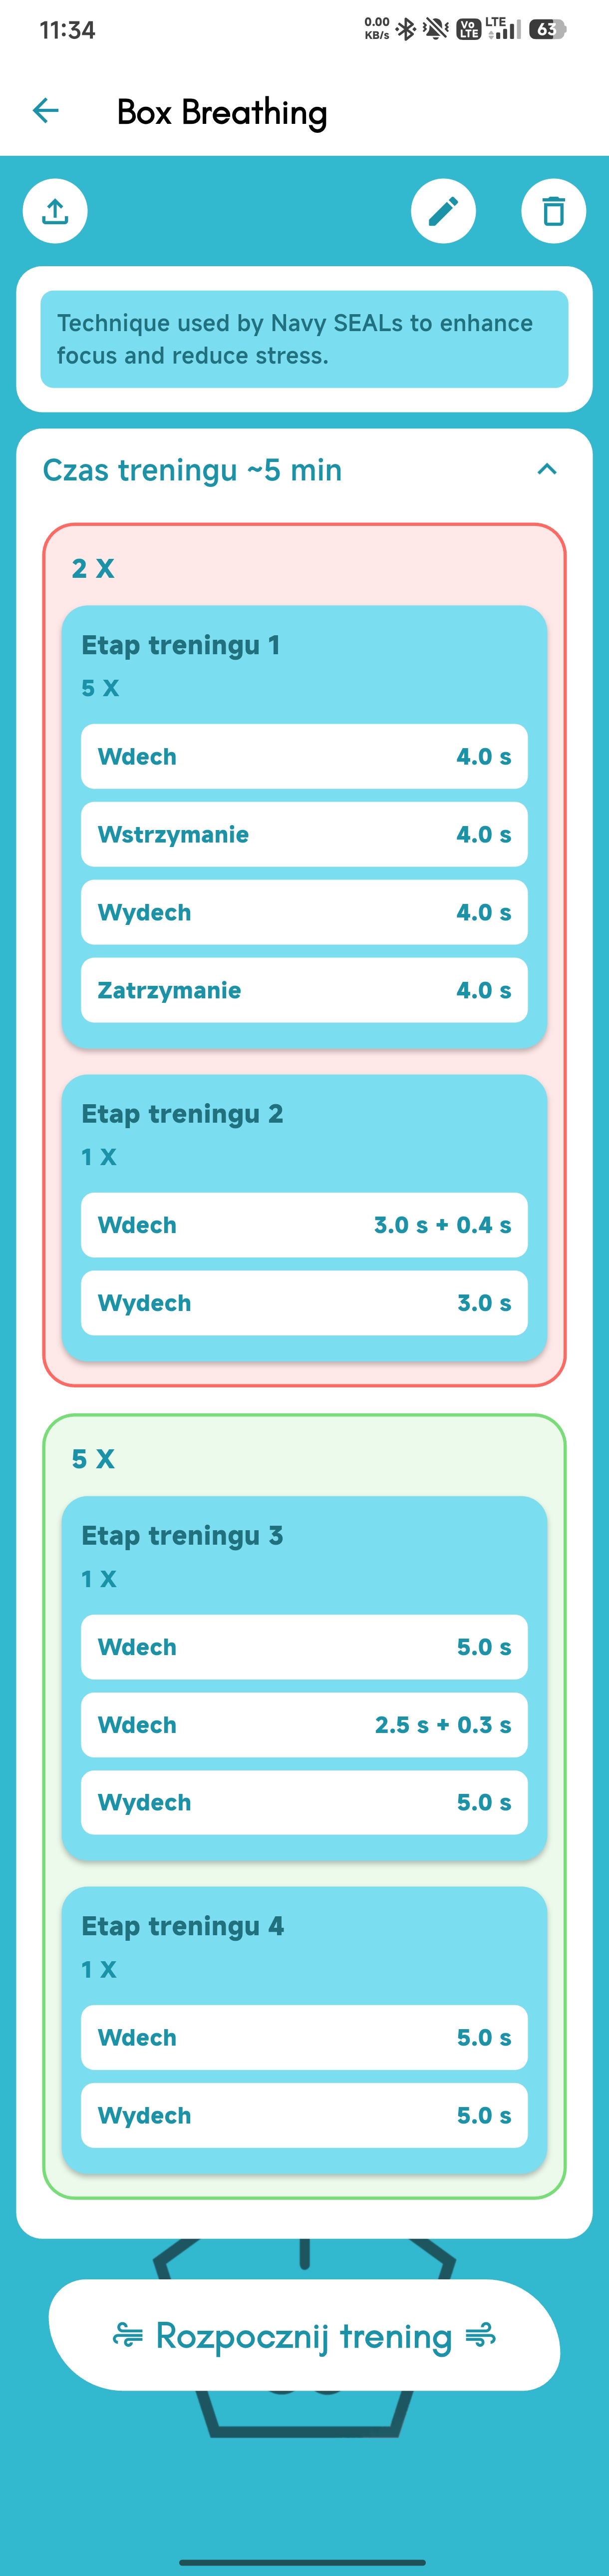
\includegraphics[width=\dimexpr\linewidth-2\fboxrule\relax,height=0.64\textheight,keepaspectratio]{obrazy/badania_interface/start_menu_new.jpg}}}
        \par\small (b)
    \end{minipage}
    \caption[Przegląd treningu przed zmianami i po rozbudowie]{Przegląd treningu: (a) ekran przed zmianami; (b) ekran po dodaniu grup oraz indywidualnych przyrostów czasu faz}
    \label{fig:ux_training_overview}
\end{figure}

\subsection{Ekran treningu oddechowego}
\label{sec:ux_breathing_visualization}

W pierwotnej wersji aplikacji przebieg treningu przedstawiano za pomocą pulsujących okręgów. Dodano alternatywną wizualizację w postaci fali na osi czasu, która pokazuje przebieg kolejnych faz oddechu. Wybór ten nawiązuje do omówionego wcześniej artykułu \textit{Evaluating mobile apps for breathing training: The effectiveness of visualization} \cite{chittaro2014evaluating}, w którym użytkownicy preferowali wizualizację falową. W odróżnieniu od kuli lub okręgu fala pozwala przedstawić także nadchodzące fazy, co było przesłanką do udostępnienia tego wariantu w aplikacji. Wyników przywołanego badania nie należy jednak utożsamiać z pomiarem skuteczności interfejsu ReSpire.

Trening można również realizować, korzystając wyłącznie ze wskazówek dźwiękowych, bez potrzeby obserwowania ekranu. Dostępne są komunikaty lektora oraz sonifikacja, czyli dźwięk narastający i opadający zgodnie z przebiegiem oddechu. Rozszerzenie to umożliwia wybór sposobu prowadzenia ćwiczenia odpowiadającego preferencjom użytkownika.

Dodano ponadto możliwość zaplanowania dwóch szybkich wdechów następujących bezpośrednio po sobie. Funkcja odpowiada na wskazaną potrzebę użytkowników i rozszerza zakres możliwych do skonfigurowania sekwencji faz oddechu. Na rysunku \ref{fig:ux_breathing_views} zestawiono pierwotną wizualizację, widok fali oraz przykład dwóch kolejnych wdechów.

\begin{figure}[H]
    \centering
    \begin{minipage}[c]{0.29\linewidth}
        \centering
        {\setlength{\fboxsep}{0pt}\setlength{\fboxrule}{0.2pt}\fcolorbox{gray}{white}{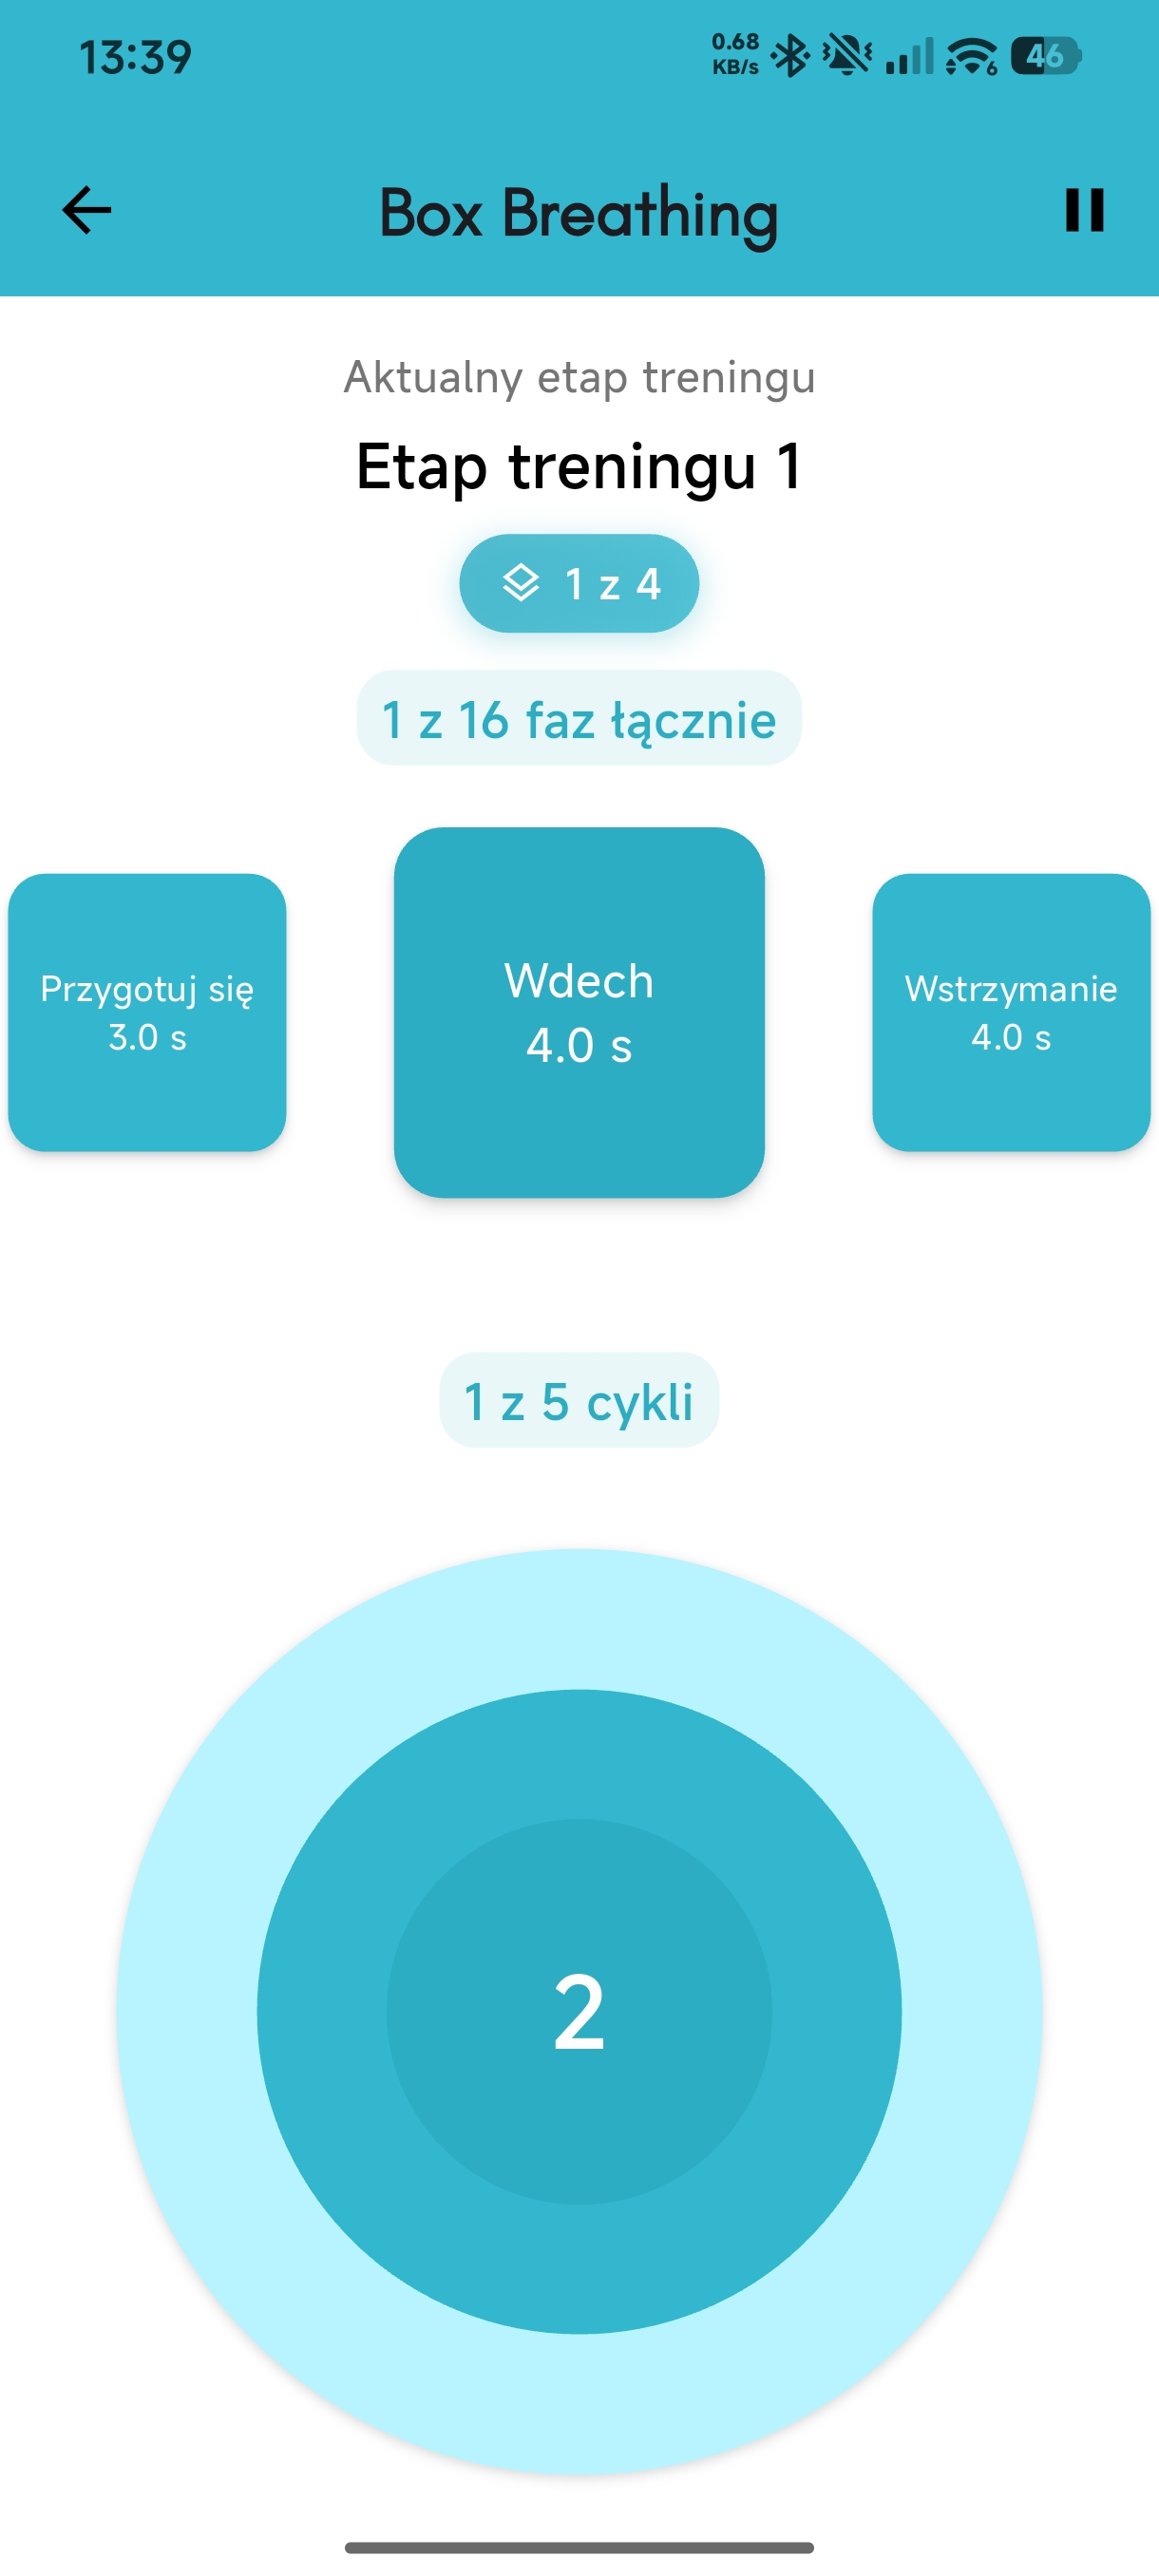
\includegraphics[width=\dimexpr\linewidth-2\fboxrule\relax]{obrazy/badania_interface/breathing_page_ring_old.jpg}}}
        \par\small (a)
    \end{minipage}\hfill
    \begin{minipage}[c]{0.06\linewidth}
        \centering
        {\large $\rightarrow$}
    \end{minipage}\hfill
    \begin{minipage}[c]{0.29\linewidth}
        \centering
        {\setlength{\fboxsep}{0pt}\setlength{\fboxrule}{0.2pt}\fcolorbox{gray}{white}{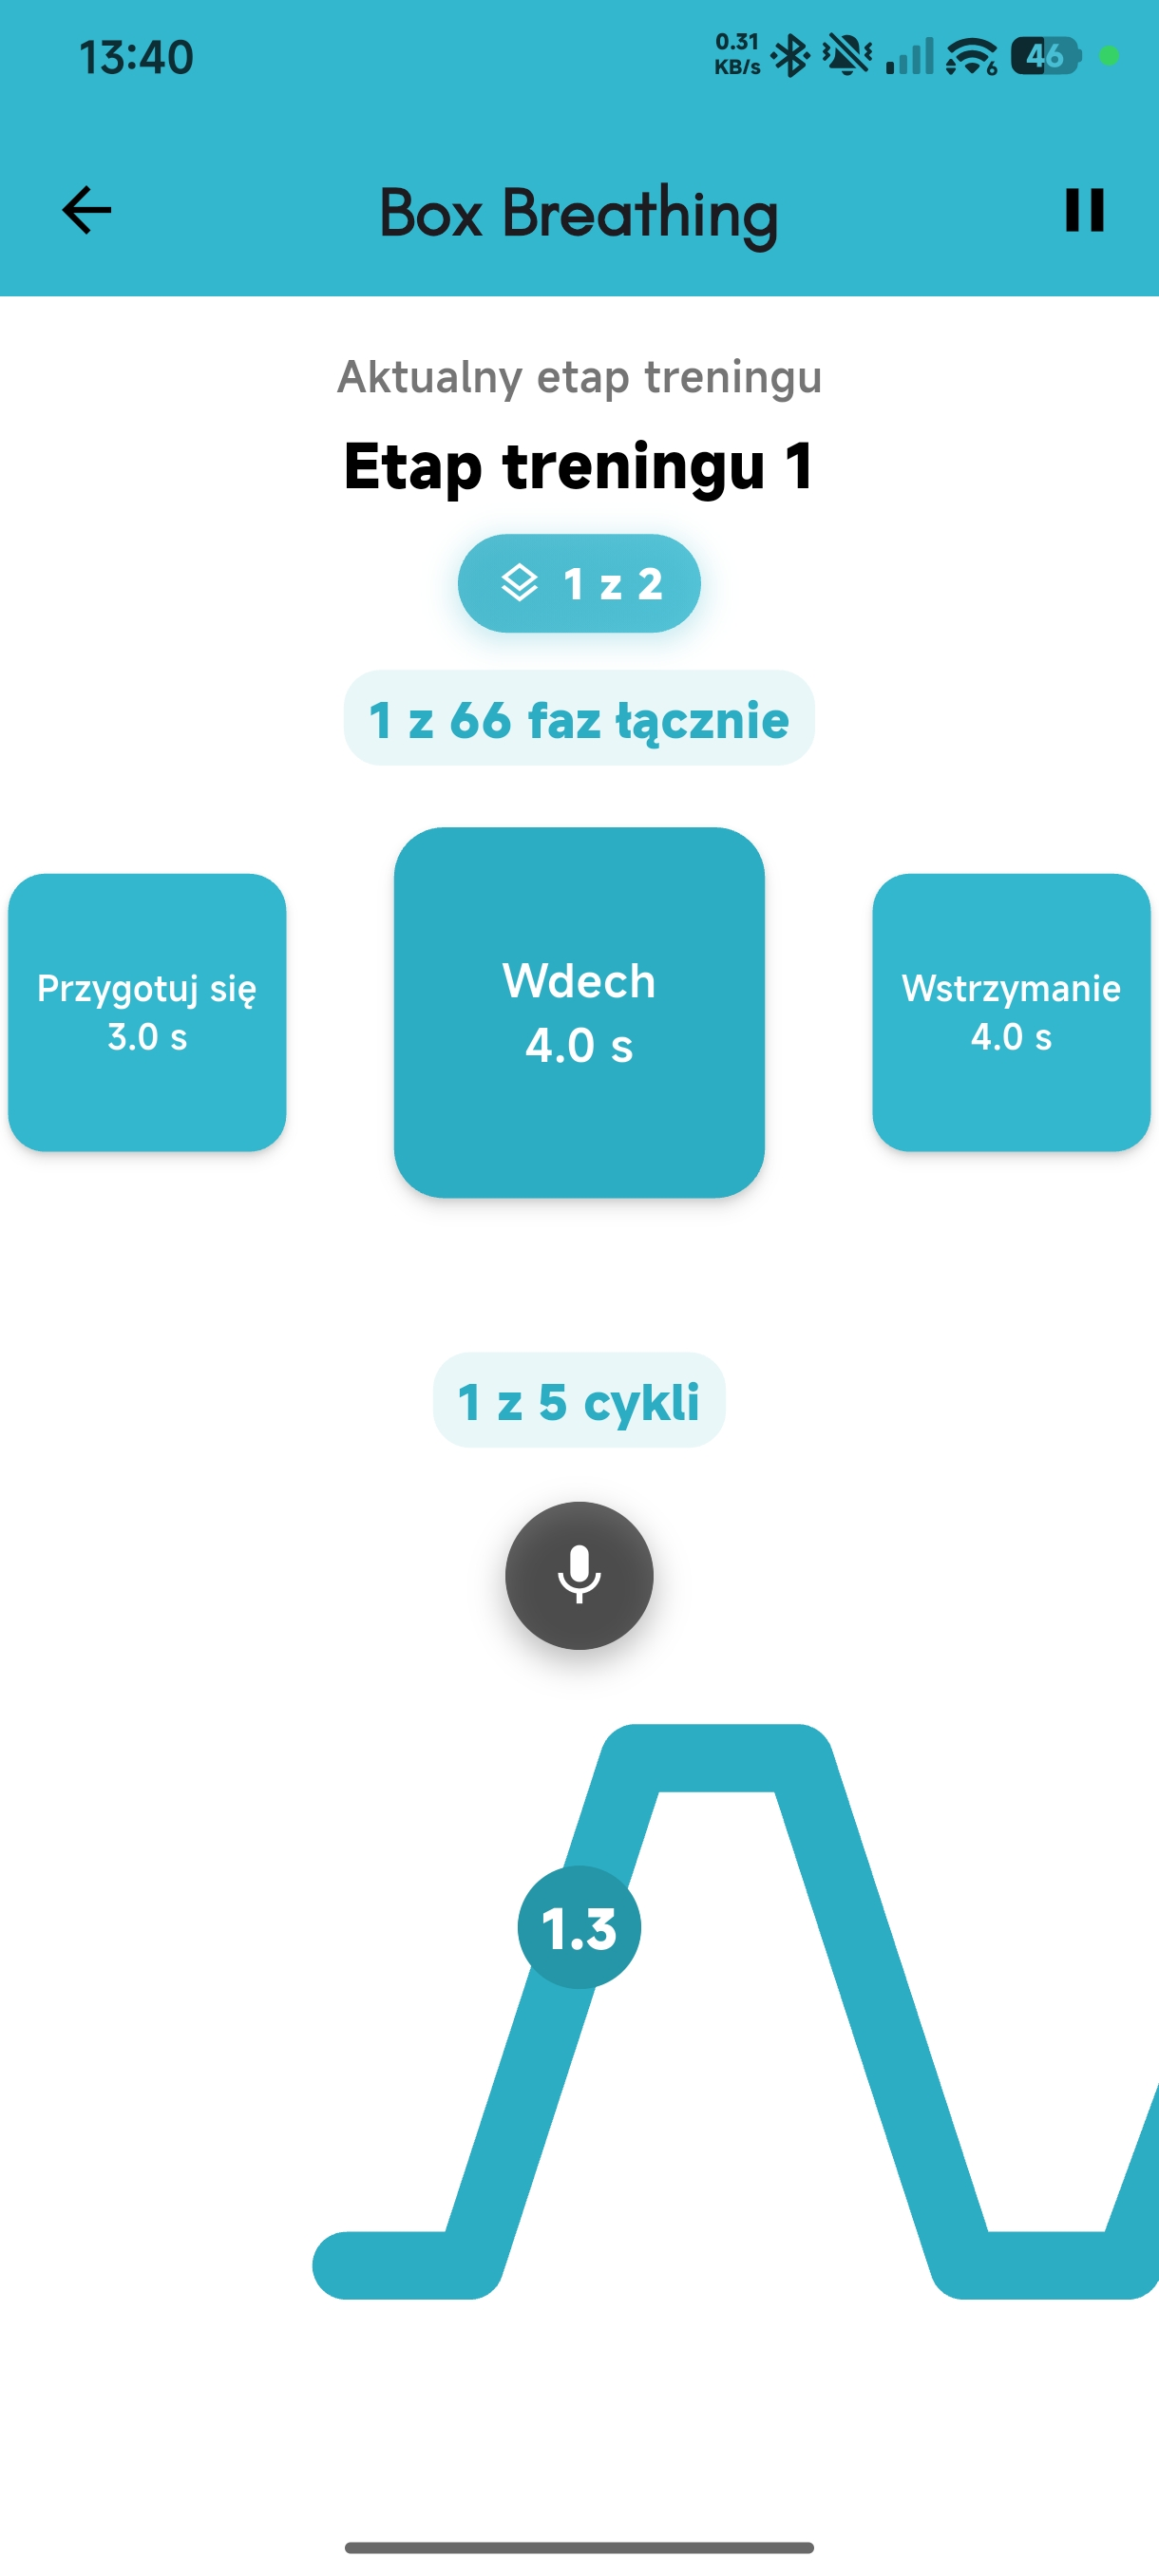
\includegraphics[width=\dimexpr\linewidth-2\fboxrule\relax]{obrazy/badania_interface/breathing_page_wave_new.jpg}}}
        \par\small (b1)
    \end{minipage}\hfill
    \begin{minipage}[c]{0.29\linewidth}
        \centering
        {\setlength{\fboxsep}{0pt}\setlength{\fboxrule}{0.2pt}\fcolorbox{gray}{white}{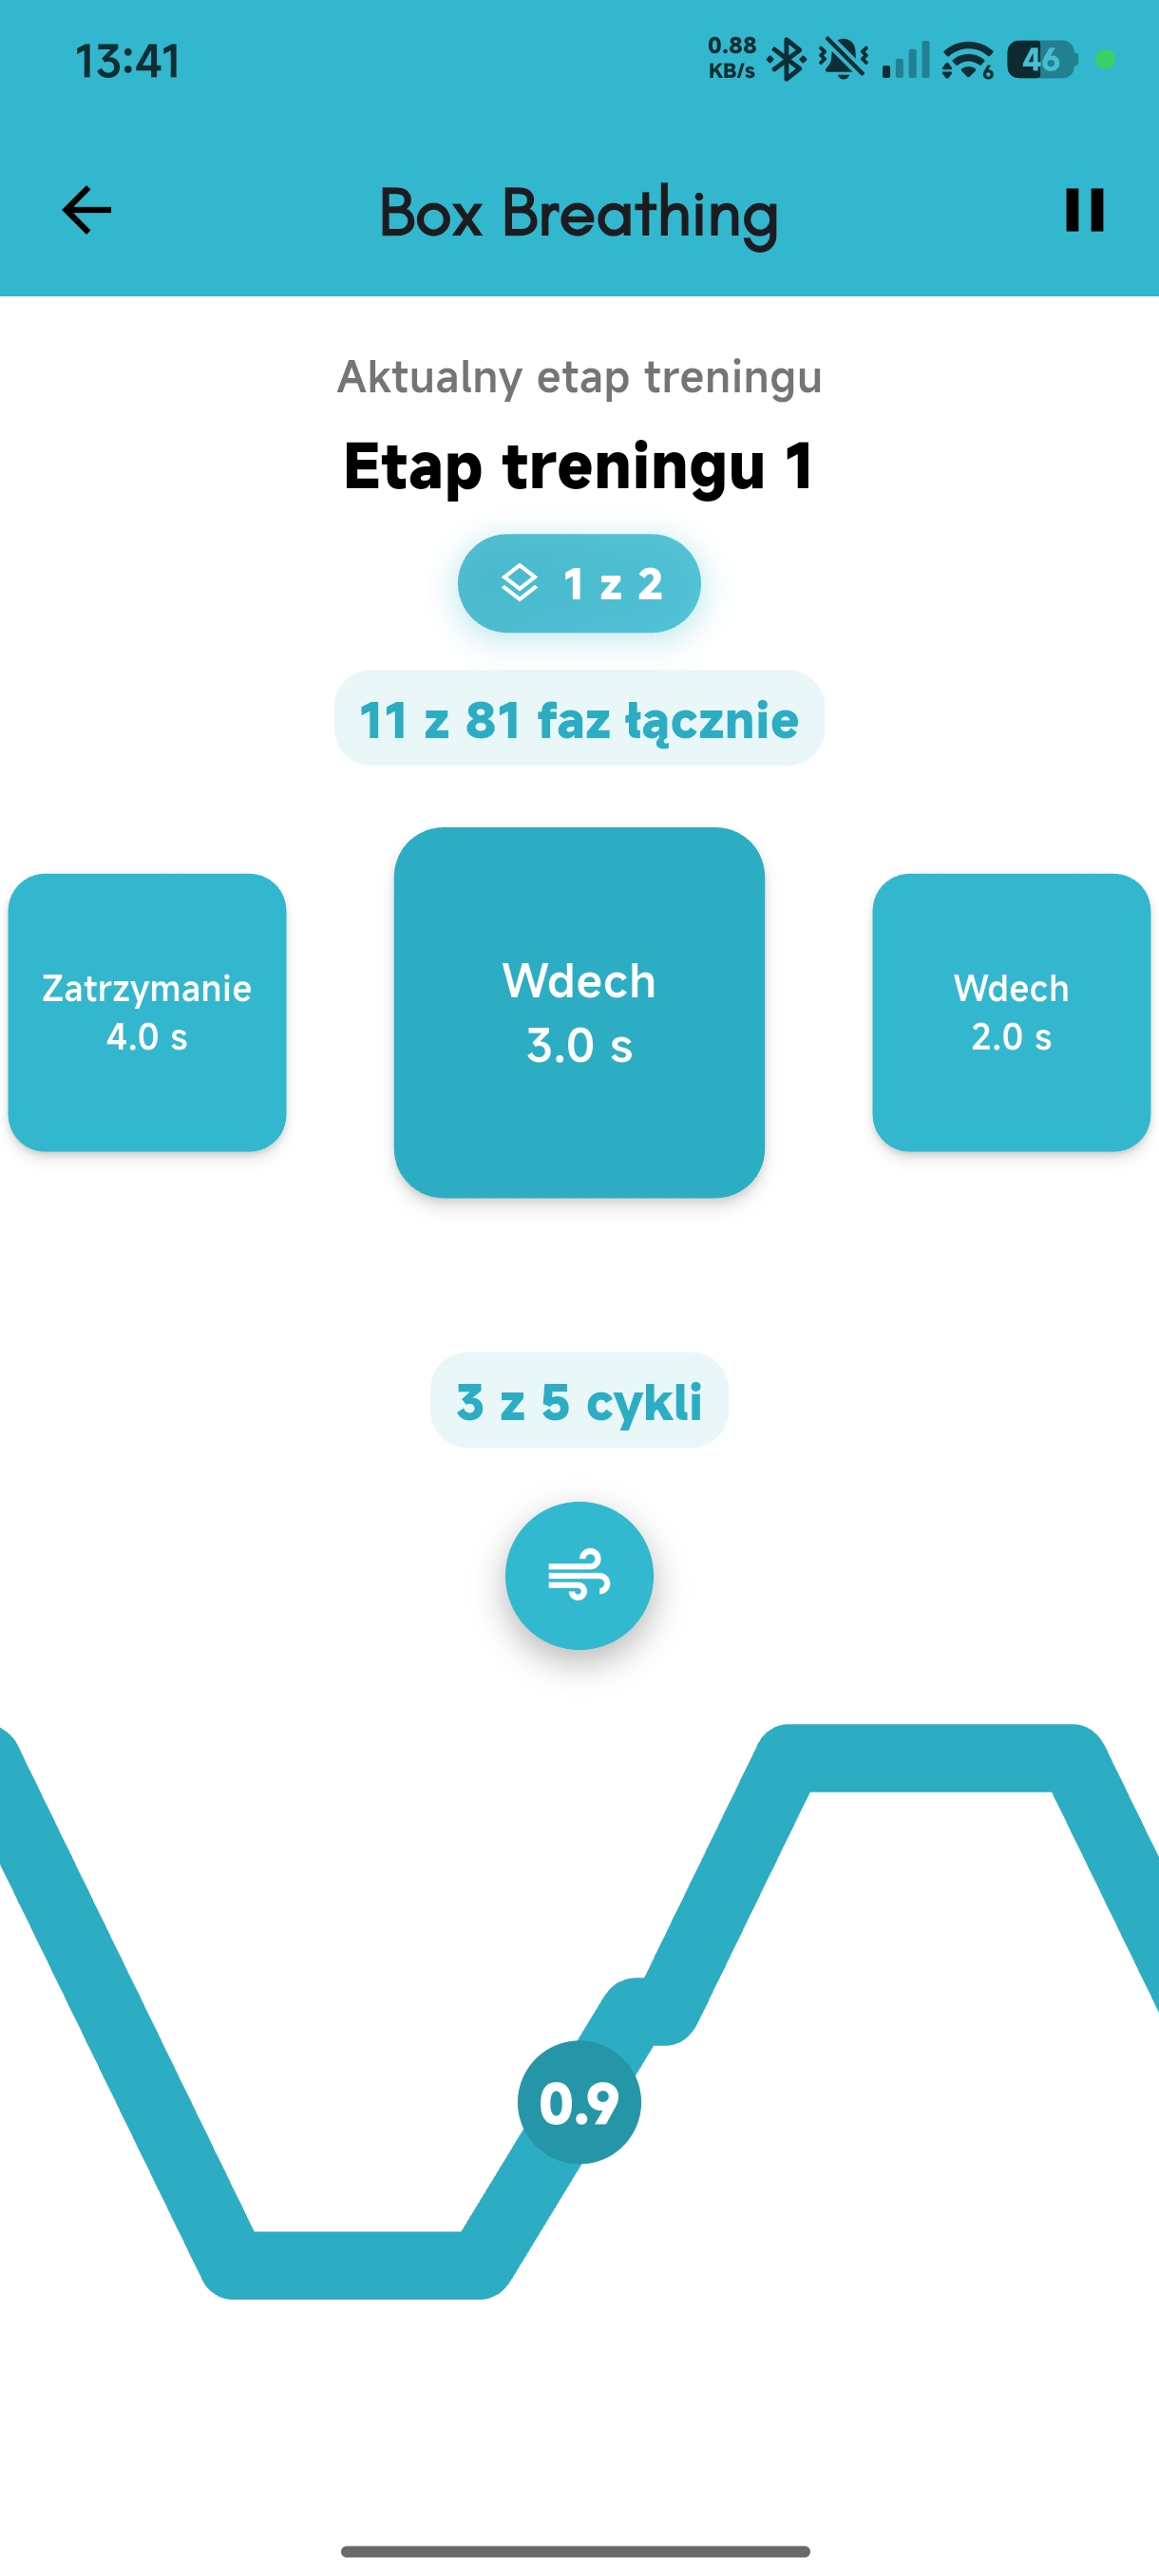
\includegraphics[width=\dimexpr\linewidth-2\fboxrule\relax]{obrazy/badania_interface/breathing_page_doube_inhale_new.jpg}}}
        \par\small (b2)
    \end{minipage}
    \caption[Porównanie sposobów wizualizacji treningu]{Wizualizacja treningu: (a) pierwotny widok okręgów; (b1) nowy widok fali; (b2) widok fali dla sekwencji dwóch kolejnych wdechów}
    \label{fig:ux_breathing_views}
\end{figure}

\subsection{Ekran edycji treningu}

Edytor rozszerzono o możliwość grupowania etapów, a także ustalania liczby powtórzeń dla konkretnej grupy. Etapy należące do danej grupy są wykonywane zgodnie z ustaloną liczbą powtórzeń przed przejściem do kolejnej grupy. Pozwala to tworzyć treningi o bardziej złożonej strukturze bez ręcznego powielania tych samych etapów. Grupy wyróżniono kolorami, a po ich utworzeniu mogą być one edytowane, łączone oraz rozdzielane.

Poprawiono również czytelność pól i etykiet, eliminując przycinanie napisów widoczne w~poprzedniej wersji. W górnej części ekranu umieszczono przybliżony czas treningu, wyznaczany na podstawie sumy czasów wszystkich zaplanowanych faz, z uwzględnieniem powtórzeń oraz zadanych przyrostów. Informacja ta umożliwia ocenę długości sesji już podczas jej konfigurowania. Na rysunku \ref{fig:ux_training_editor} przedstawiono poprzedni ekran i kolejne fragmenty rozbudowanego edytora.

\begin{figure}[H]
    \centering
    \begin{minipage}{0.31\linewidth}
        \centering
        {\setlength{\fboxsep}{0pt}\setlength{\fboxrule}{0.2pt}\fcolorbox{gray}{white}{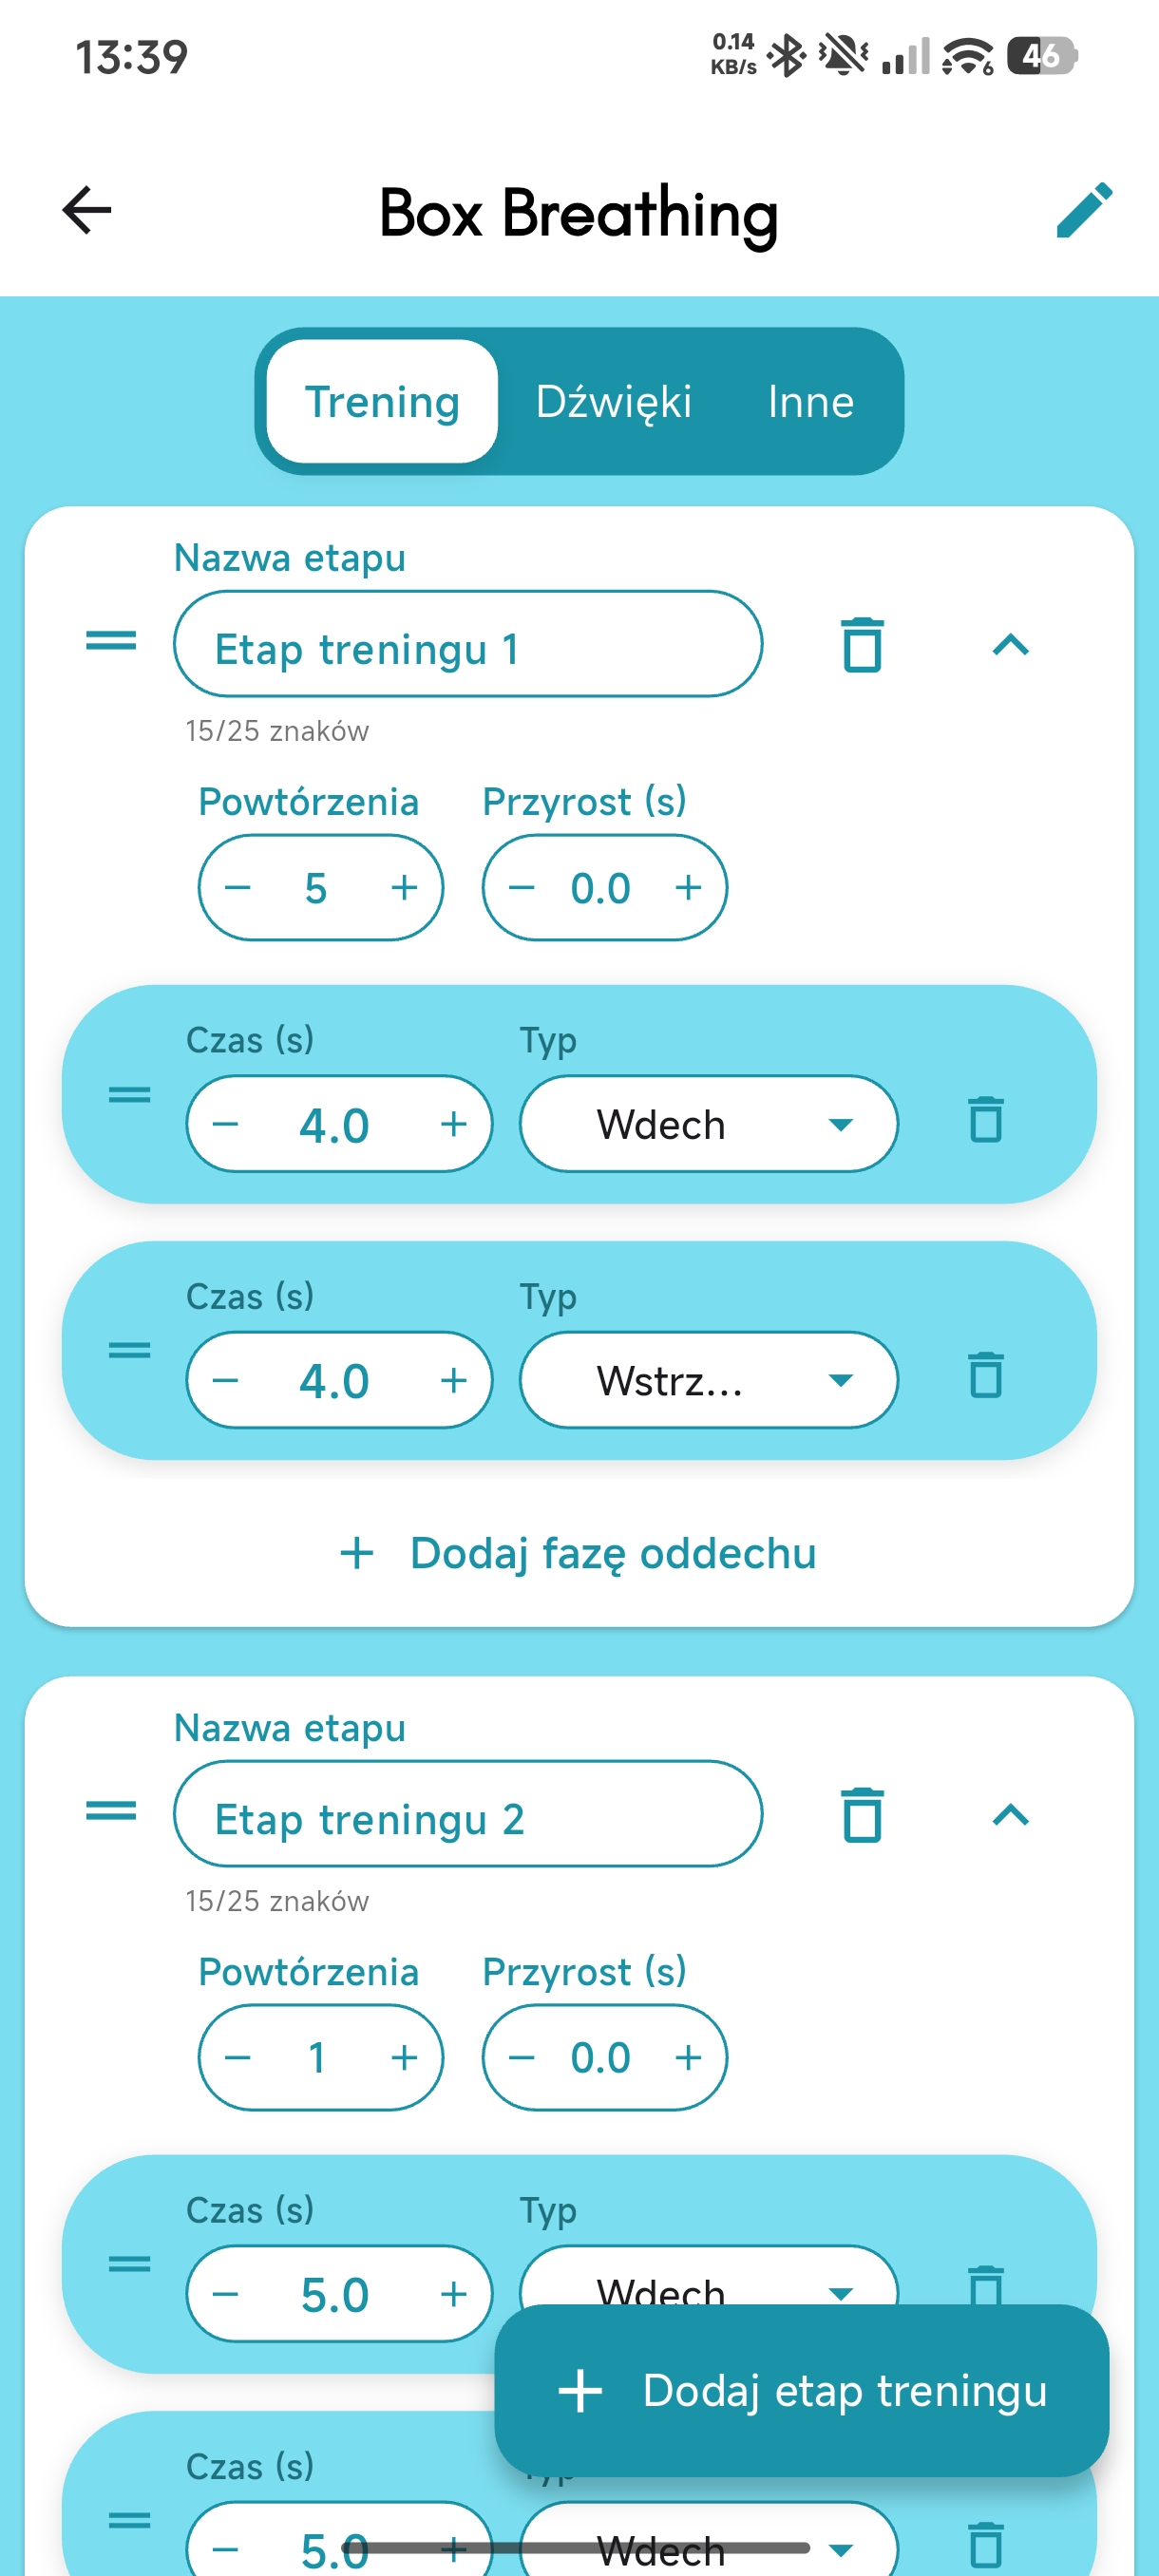
\includegraphics[width=\dimexpr\linewidth-2\fboxrule\relax]{obrazy/badania_interface/trening_edit_old.jpg}}}
        \par\small (a)
    \end{minipage}
    \par\vspace{1pt}
    {\large $\downarrow$}\par
    \vspace{1pt}
    \begin{minipage}[t]{0.31\linewidth}
        \centering
        {\setlength{\fboxsep}{0pt}\setlength{\fboxrule}{0.2pt}\fcolorbox{gray}{white}{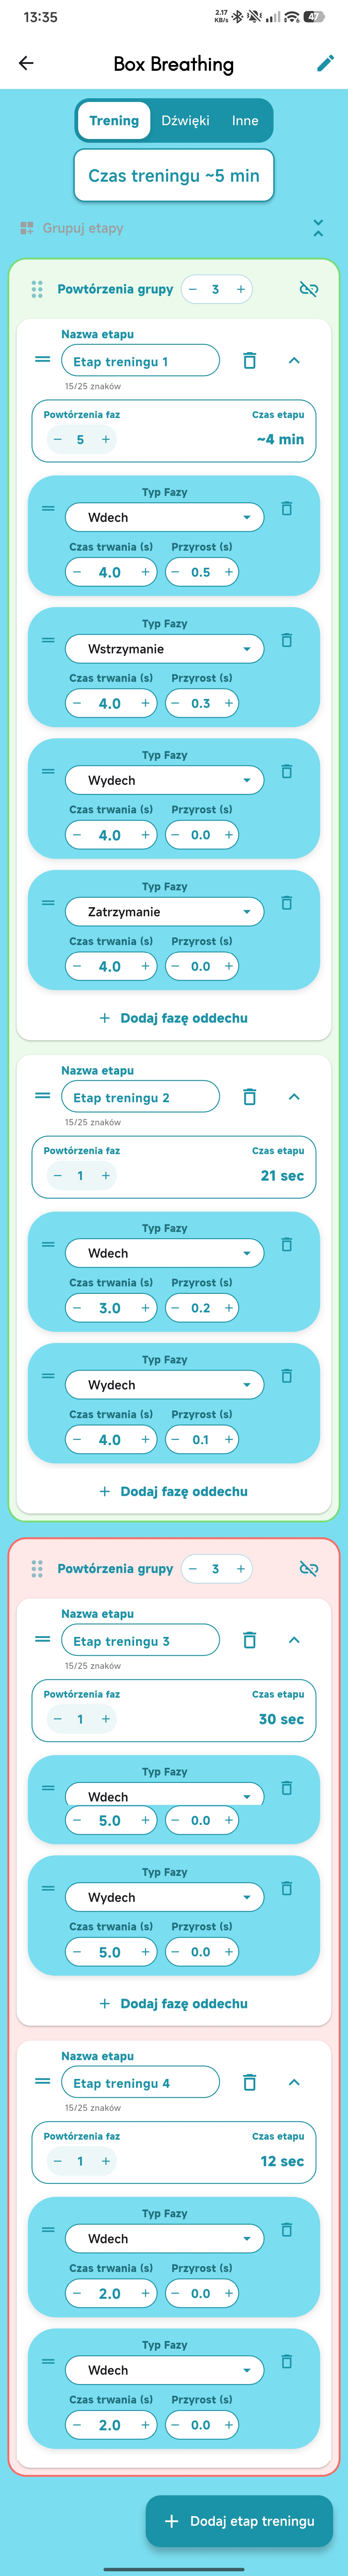
\includegraphics[width=\dimexpr\linewidth-2\fboxrule\relax,trim={0 6022bp 0 0},clip]{obrazy/badania_interface/trening_edit_new.jpg}}}
        \par\small (b1)
    \end{minipage}\hfill
    \begin{minipage}[t]{0.31\linewidth}
        \centering
        {\setlength{\fboxsep}{0pt}\setlength{\fboxrule}{0.2pt}\fcolorbox{gray}{white}{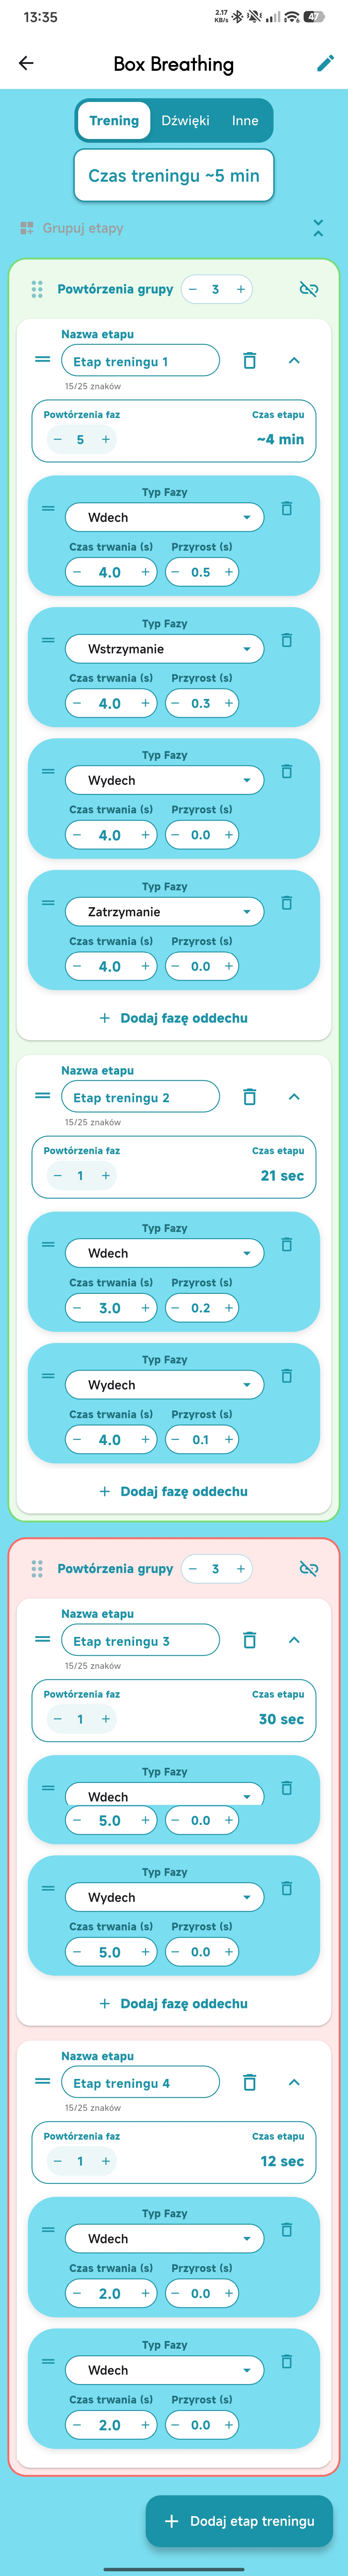
\includegraphics[width=\dimexpr\linewidth-2\fboxrule\relax,trim={0 3011bp 0 3011bp},clip]{obrazy/badania_interface/trening_edit_new.jpg}}}
        \par\small (b2)
    \end{minipage}\hfill
    \begin{minipage}[t]{0.31\linewidth}
        \centering
        {\setlength{\fboxsep}{0pt}\setlength{\fboxrule}{0.2pt}\fcolorbox{gray}{white}{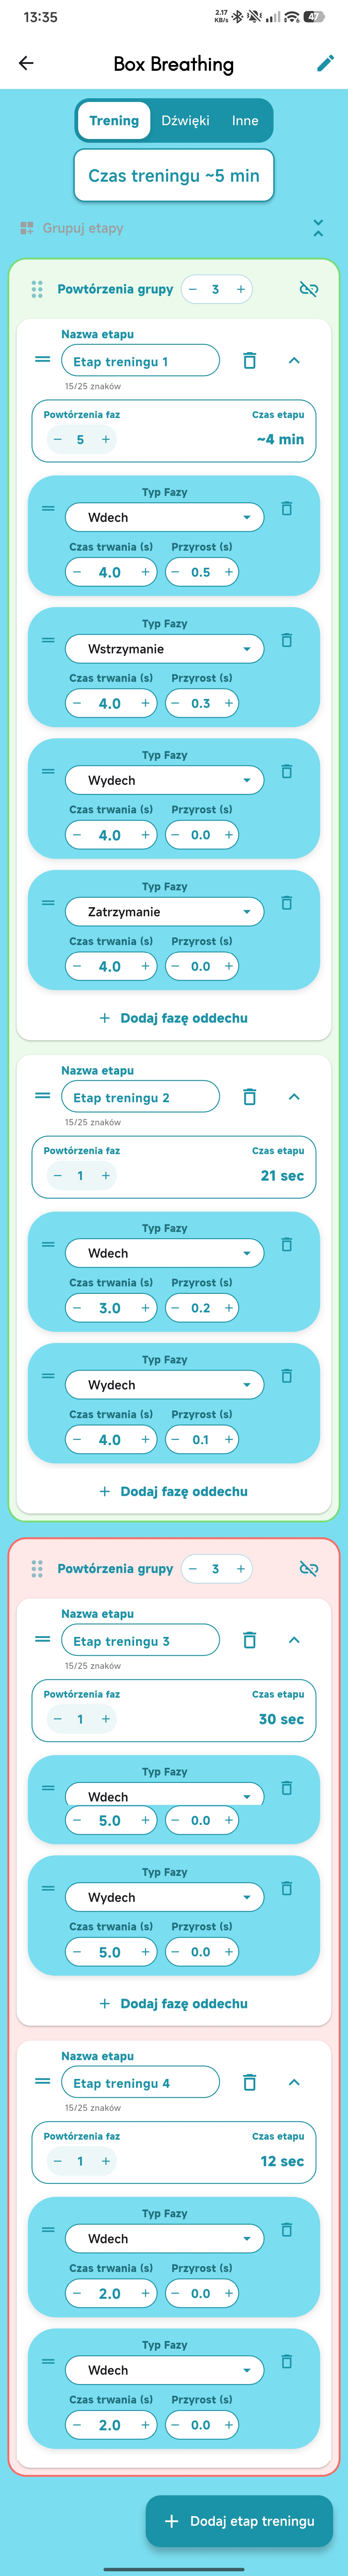
\includegraphics[width=\dimexpr\linewidth-2\fboxrule\relax,trim={0 0 0 6022bp},clip]{obrazy/badania_interface/trening_edit_new.jpg}}}
        \par\small (b3)
    \end{minipage}
    \caption[Edycja treningu przed zmianami i po rozbudowie interfejsu]{Edycja treningu: (a) ekran przed zmianami; (b1) górna część nowego ekranu z czasem treningu i ustawieniami grupy; (b2) środkowa część z kolejnymi etapami i podziałem na grupy; (b3) dolna część z ustawieniami faz oraz przyciskiem dodawania etapu}
    \label{fig:ux_training_editor}
\end{figure}

\subsection{Ekran edycji dźwięku}

W ustawieniach dźwięku ujednolicono styl komponentów, tak aby pola wyboru, suwaki i~przyciski tworzyły spójny interfejs. Ustawienia dźwięków rozpoczęcia oraz zakończenia treningu przeniesiono do zakładki \textit{Inne}, w której znajdują się również parametry czasowe tych części sesji. Rozszerzono ponadto zestaw dostępnych dźwięków. Porównanie ustawień muzyki, a także sygnałów treningowych przedstawiono na rysunku \ref{fig:ux_music_settings}.

\begin{figure}[H]
    \centering
    \begin{minipage}[c]{0.44\linewidth}
        \centering
        {\setlength{\fboxsep}{0pt}\setlength{\fboxrule}{0.2pt}\fcolorbox{gray}{white}{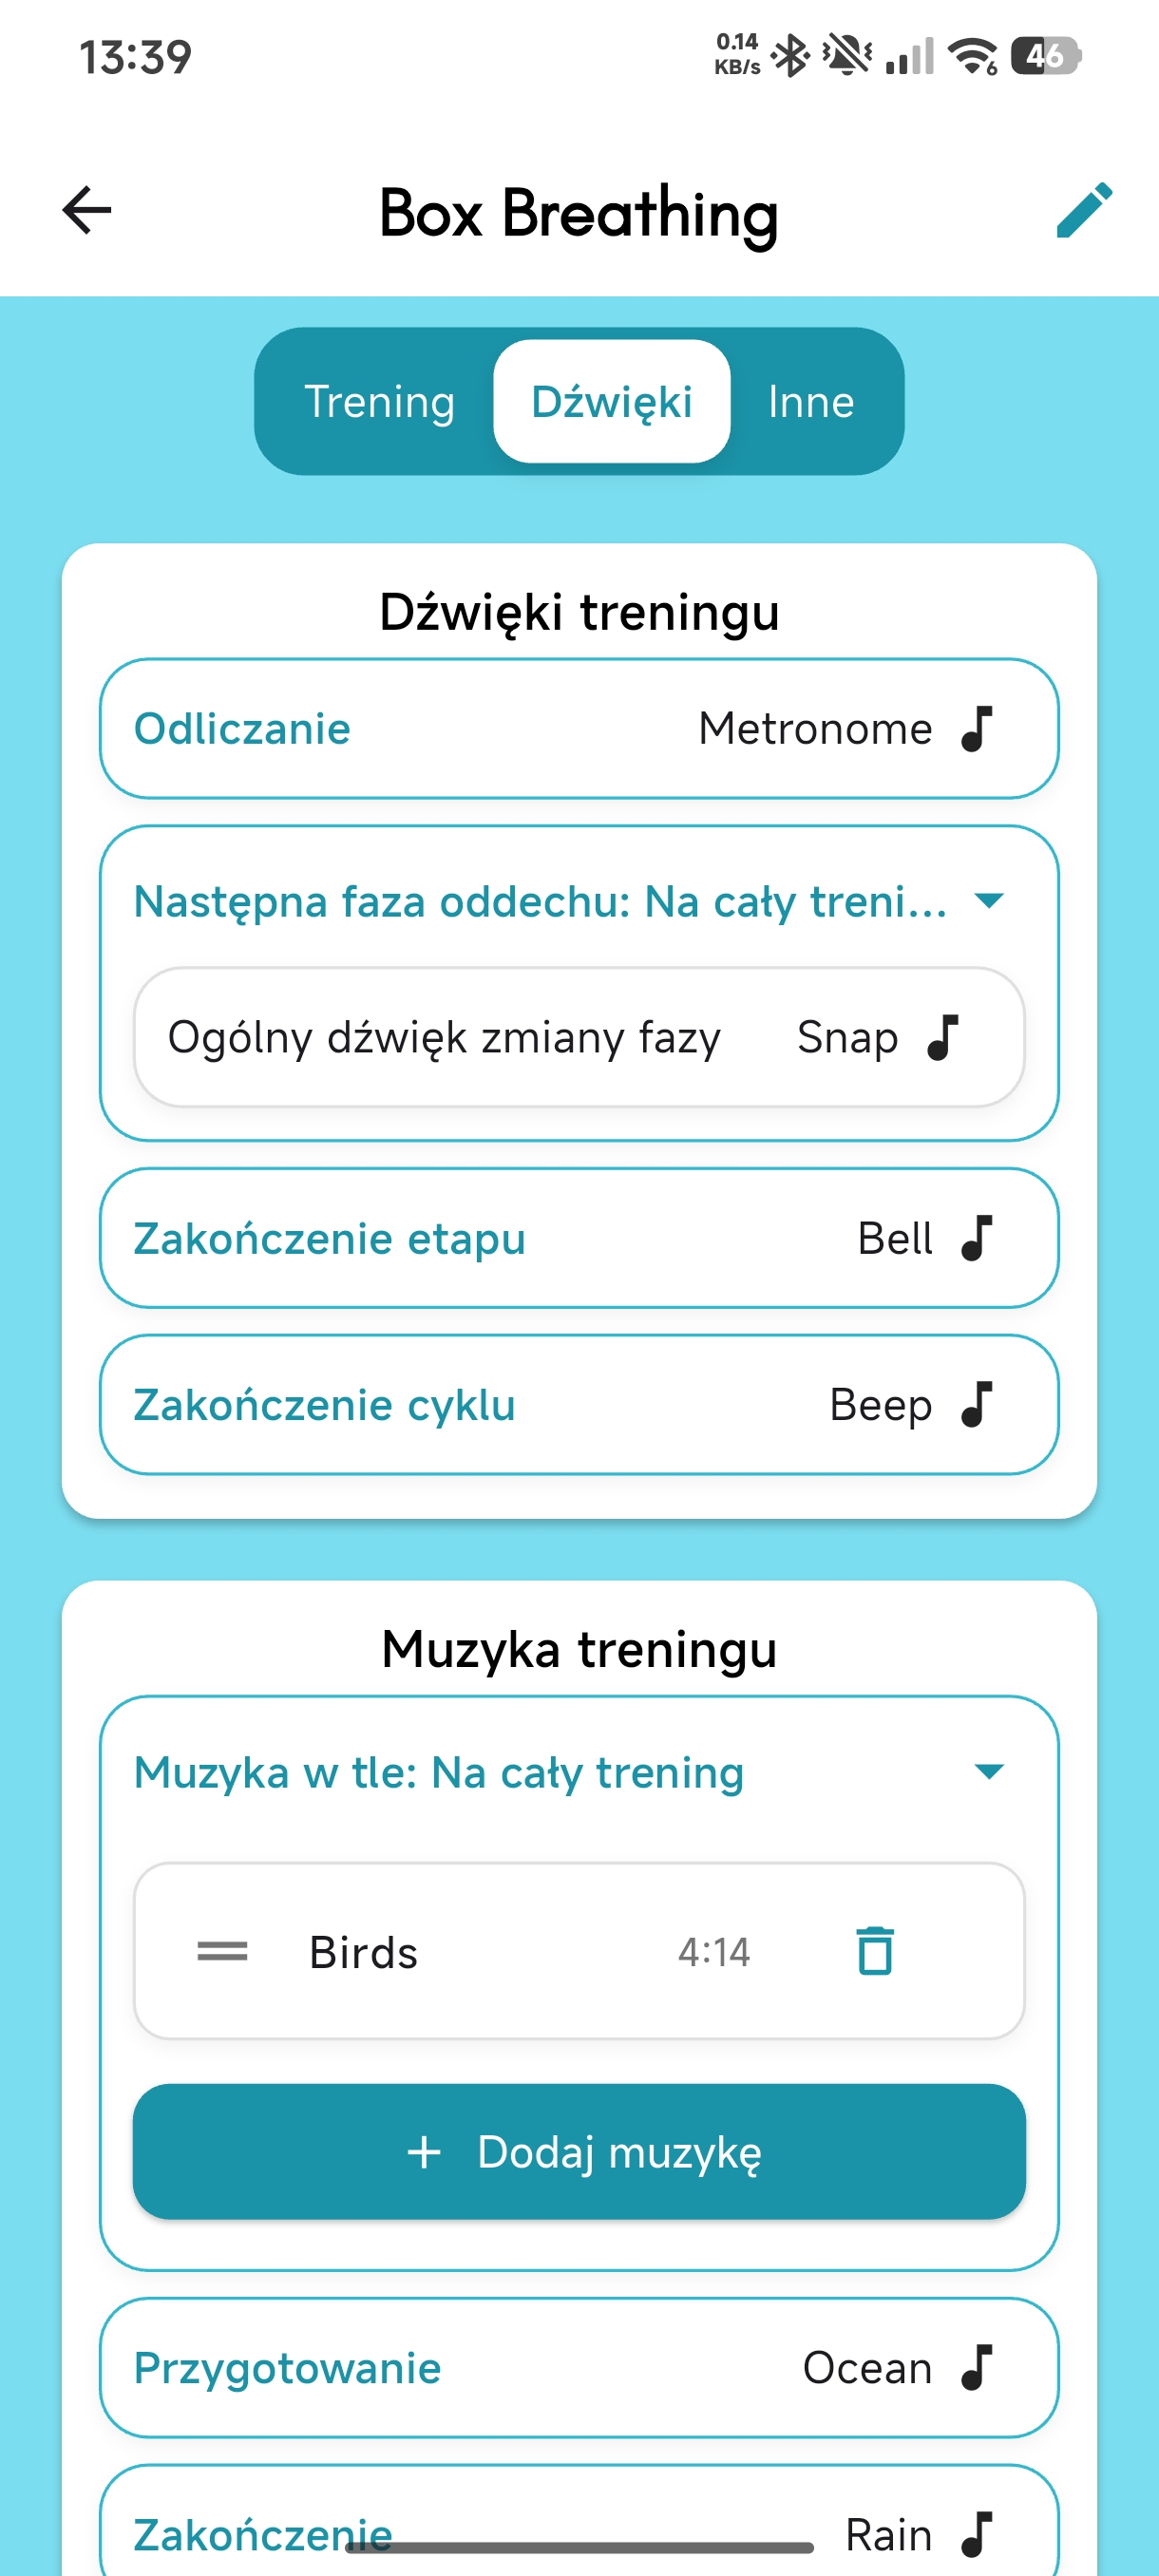
\includegraphics[width=\dimexpr\linewidth-2\fboxrule\relax,height=0.62\textheight,keepaspectratio]{obrazy/badania_interface/sound_settings_old_music.jpg}}}
        \par\small (a)
    \end{minipage}\hfill
    \begin{minipage}[c]{0.08\linewidth}
        \centering
        {\large $\rightarrow$}
    \end{minipage}\hfill
    \begin{minipage}[c]{0.44\linewidth}
        \centering
        {\setlength{\fboxsep}{0pt}\setlength{\fboxrule}{0.2pt}\fcolorbox{gray}{white}{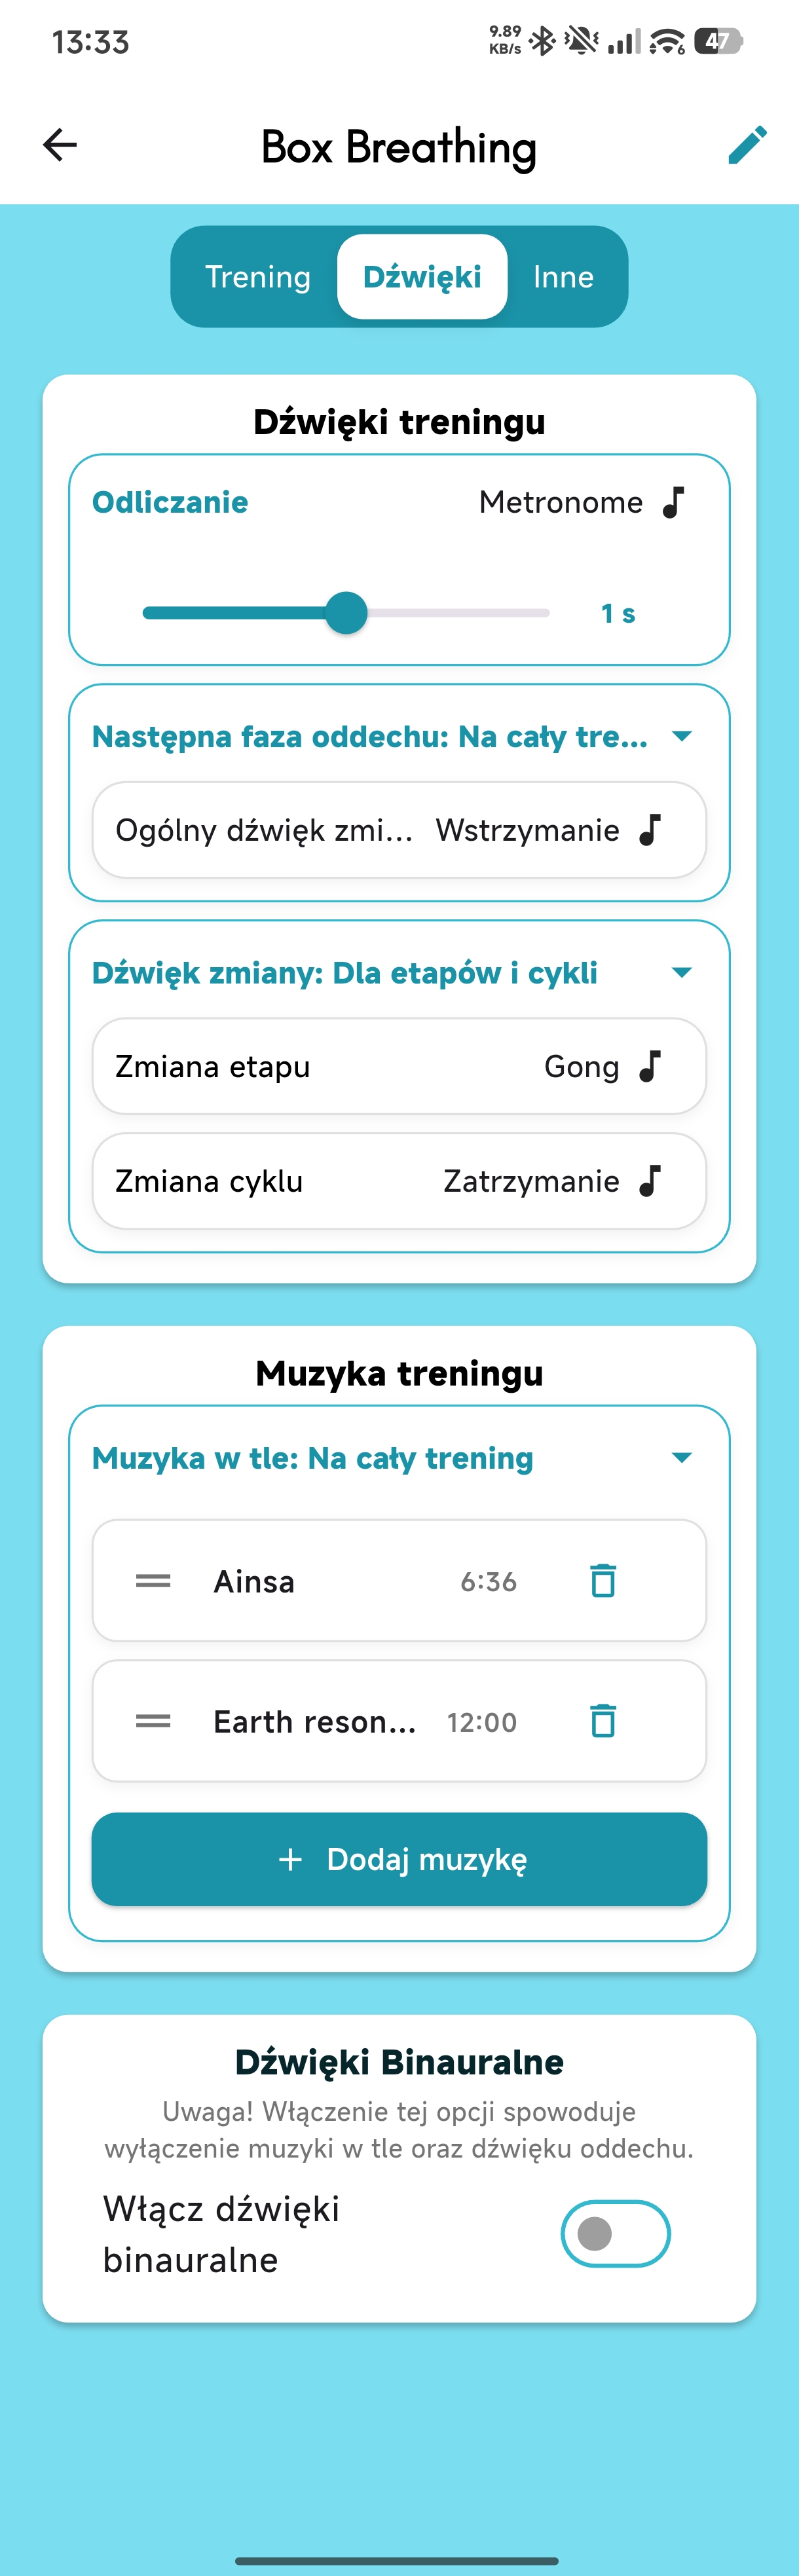
\includegraphics[width=\dimexpr\linewidth-2\fboxrule\relax,height=0.62\textheight,keepaspectratio]{obrazy/badania_interface/sounds_settings_new_music.jpg}}}
        \par\small (b)
    \end{minipage}
    \caption[Ustawienia muzyki i sygnałów dźwiękowych przed zmianami i po reorganizacji]{Ustawienia muzyki i sygnałów dźwiękowych: (a) ekran przed zmianami; (b) ekran po ujednoliceniu komponentów i reorganizacji ustawień}
    \label{fig:ux_music_settings}
\end{figure}

Zmieniono również sposób konfiguracji dźwięków binauralnych. Zamiast niezależnie ustawiać częstotliwość dla lewego i prawego ucha, użytkownik wybiera częstotliwość bazową oraz różnicę częstotliwości. Ekran wskazuje kategorię odpowiadającą wybranej różnicy zgodnej z częstotliwościami Solfeggio, na przykład alpha, beta lub gamma. Są to dźwięki, które mogą w różny sposób wpływać na doświadczenia użytkownika podczas sesji ćwiczeń oddechu. Odpowiednie konfiguracje mogą pomóc w zrelaksowaniu się lub pobudzeniu organizmu. Nowy interfejs pozwala dobierać ustawienie bez samodzielnego obliczania różnicy pomiędzy kanałami. Oba warianty konfiguracji przedstawiono na rysunku \ref{fig:ux_binaural_settings}.

W aplikacji muzyka w tle oraz dźwięki binauralne są trybami wzajemnie wykluczającymi się. Aktywowanie dźwięków binauralnych wymaga wyłączenia muzyki, natomiast uruchomienie muzyki wyklucza jednoczesne korzystanie z dźwięków binauralnych.

\begin{figure}[H]
    \centering
    \begin{minipage}[c]{0.44\linewidth}
        \centering
        {\setlength{\fboxsep}{0pt}\setlength{\fboxrule}{0.2pt}\fcolorbox{gray}{white}{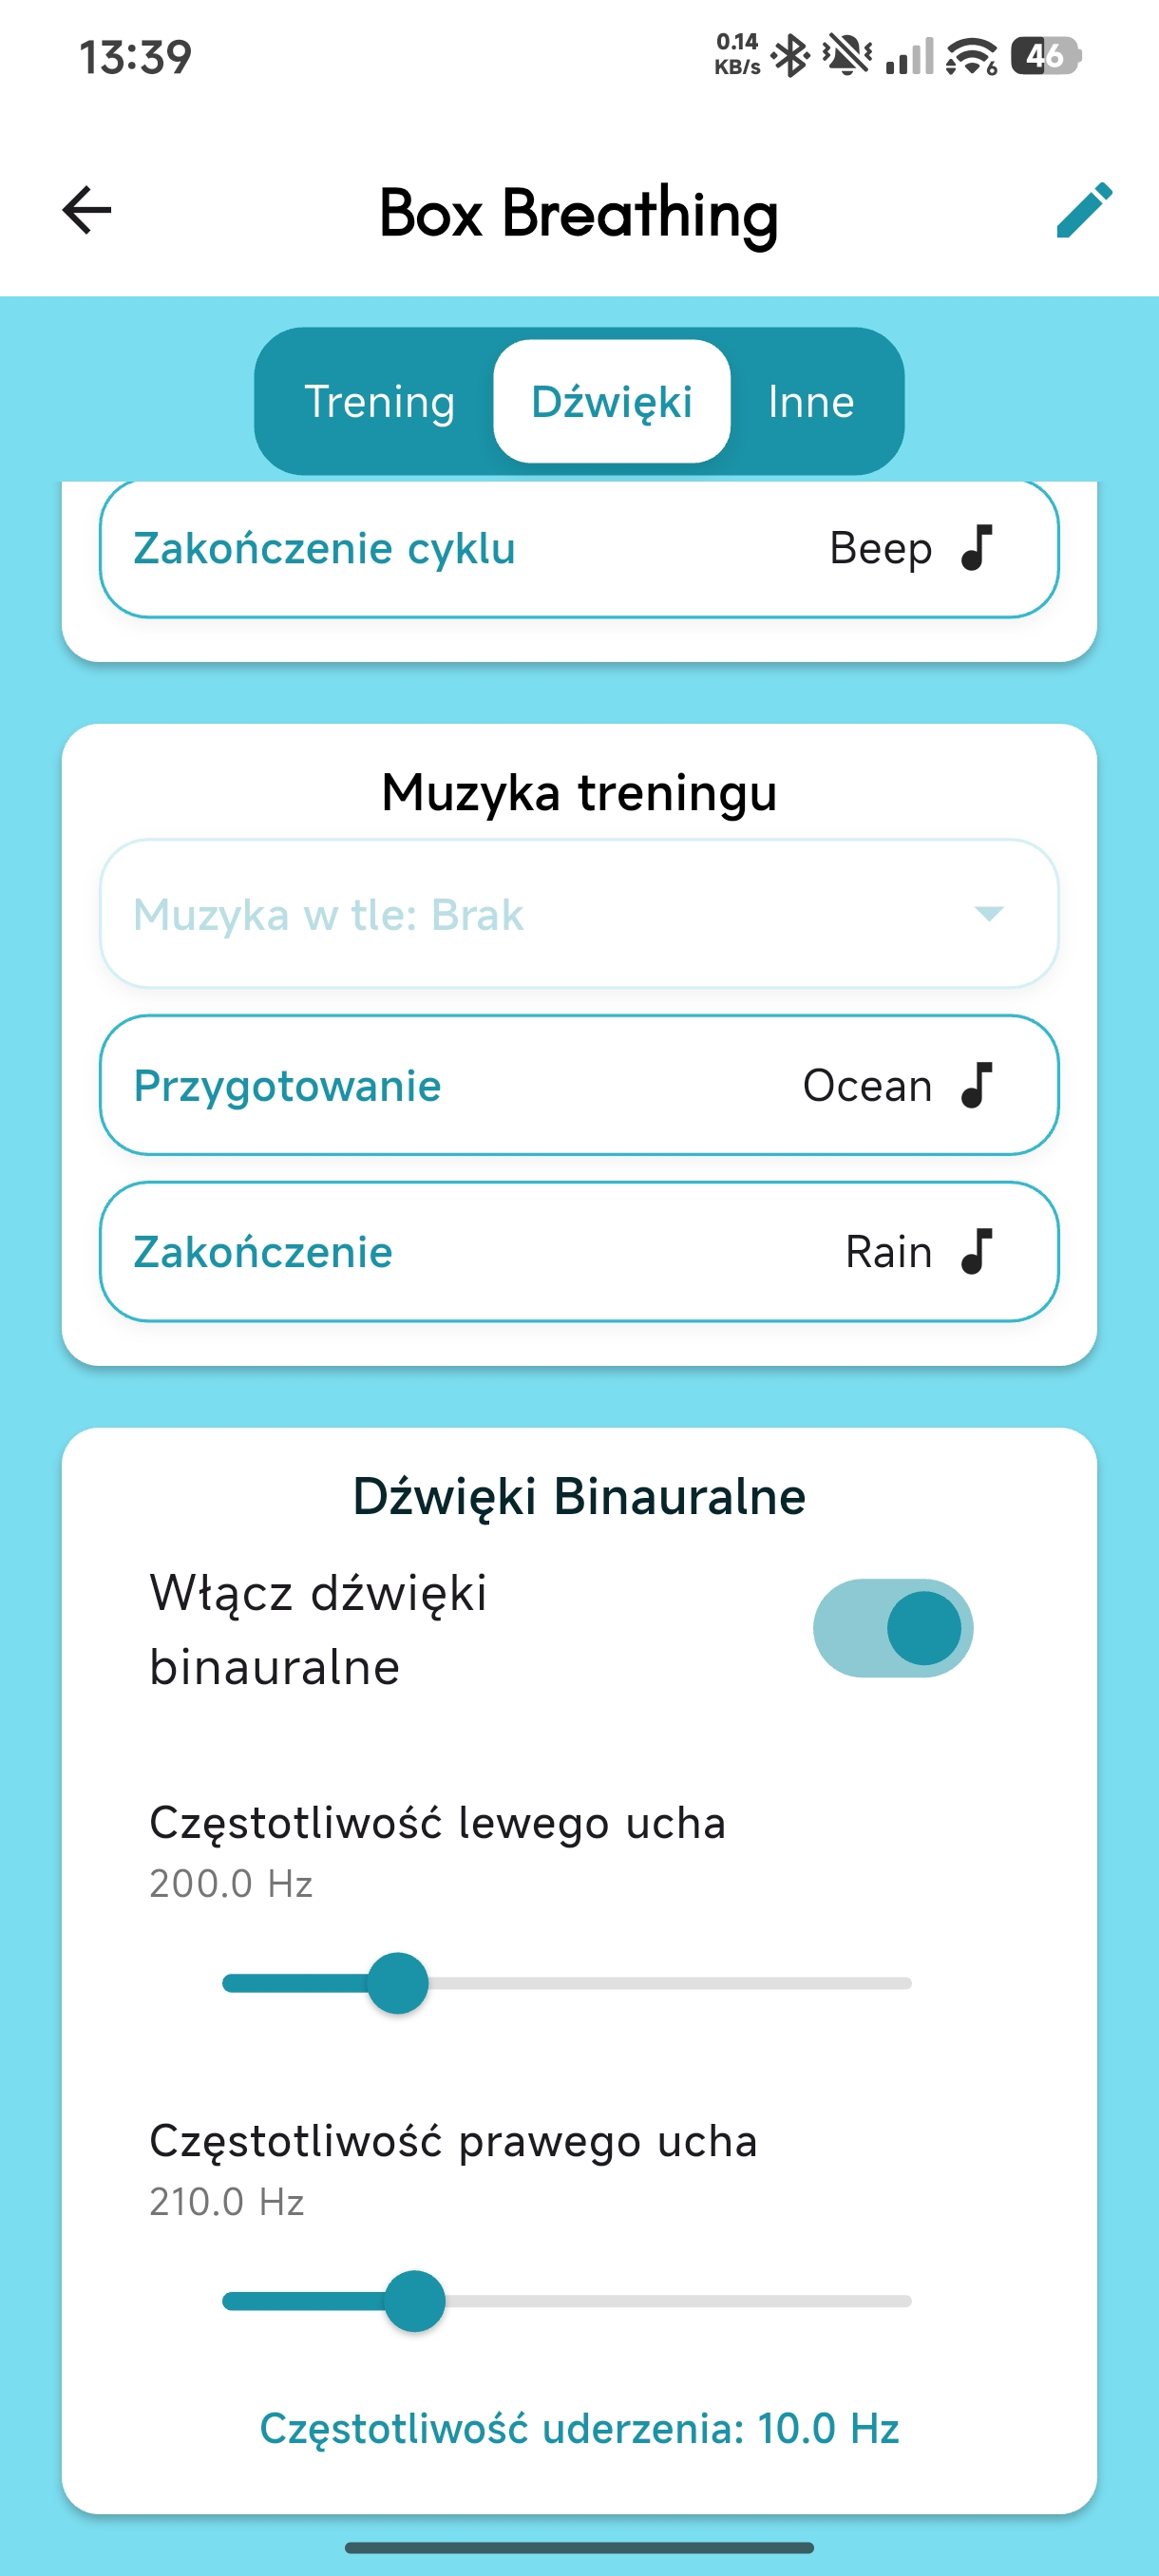
\includegraphics[width=\dimexpr\linewidth-2\fboxrule\relax,height=0.57\textheight,keepaspectratio]{obrazy/badania_interface/sound_settings_old_binaural.jpg}}}
        \par\small (a)
    \end{minipage}\hfill
    \begin{minipage}[c]{0.08\linewidth}
        \centering
        {\large $\rightarrow$}
    \end{minipage}\hfill
    \begin{minipage}[c]{0.44\linewidth}
        \centering
        {\setlength{\fboxsep}{0pt}\setlength{\fboxrule}{0.2pt}\fcolorbox{gray}{white}{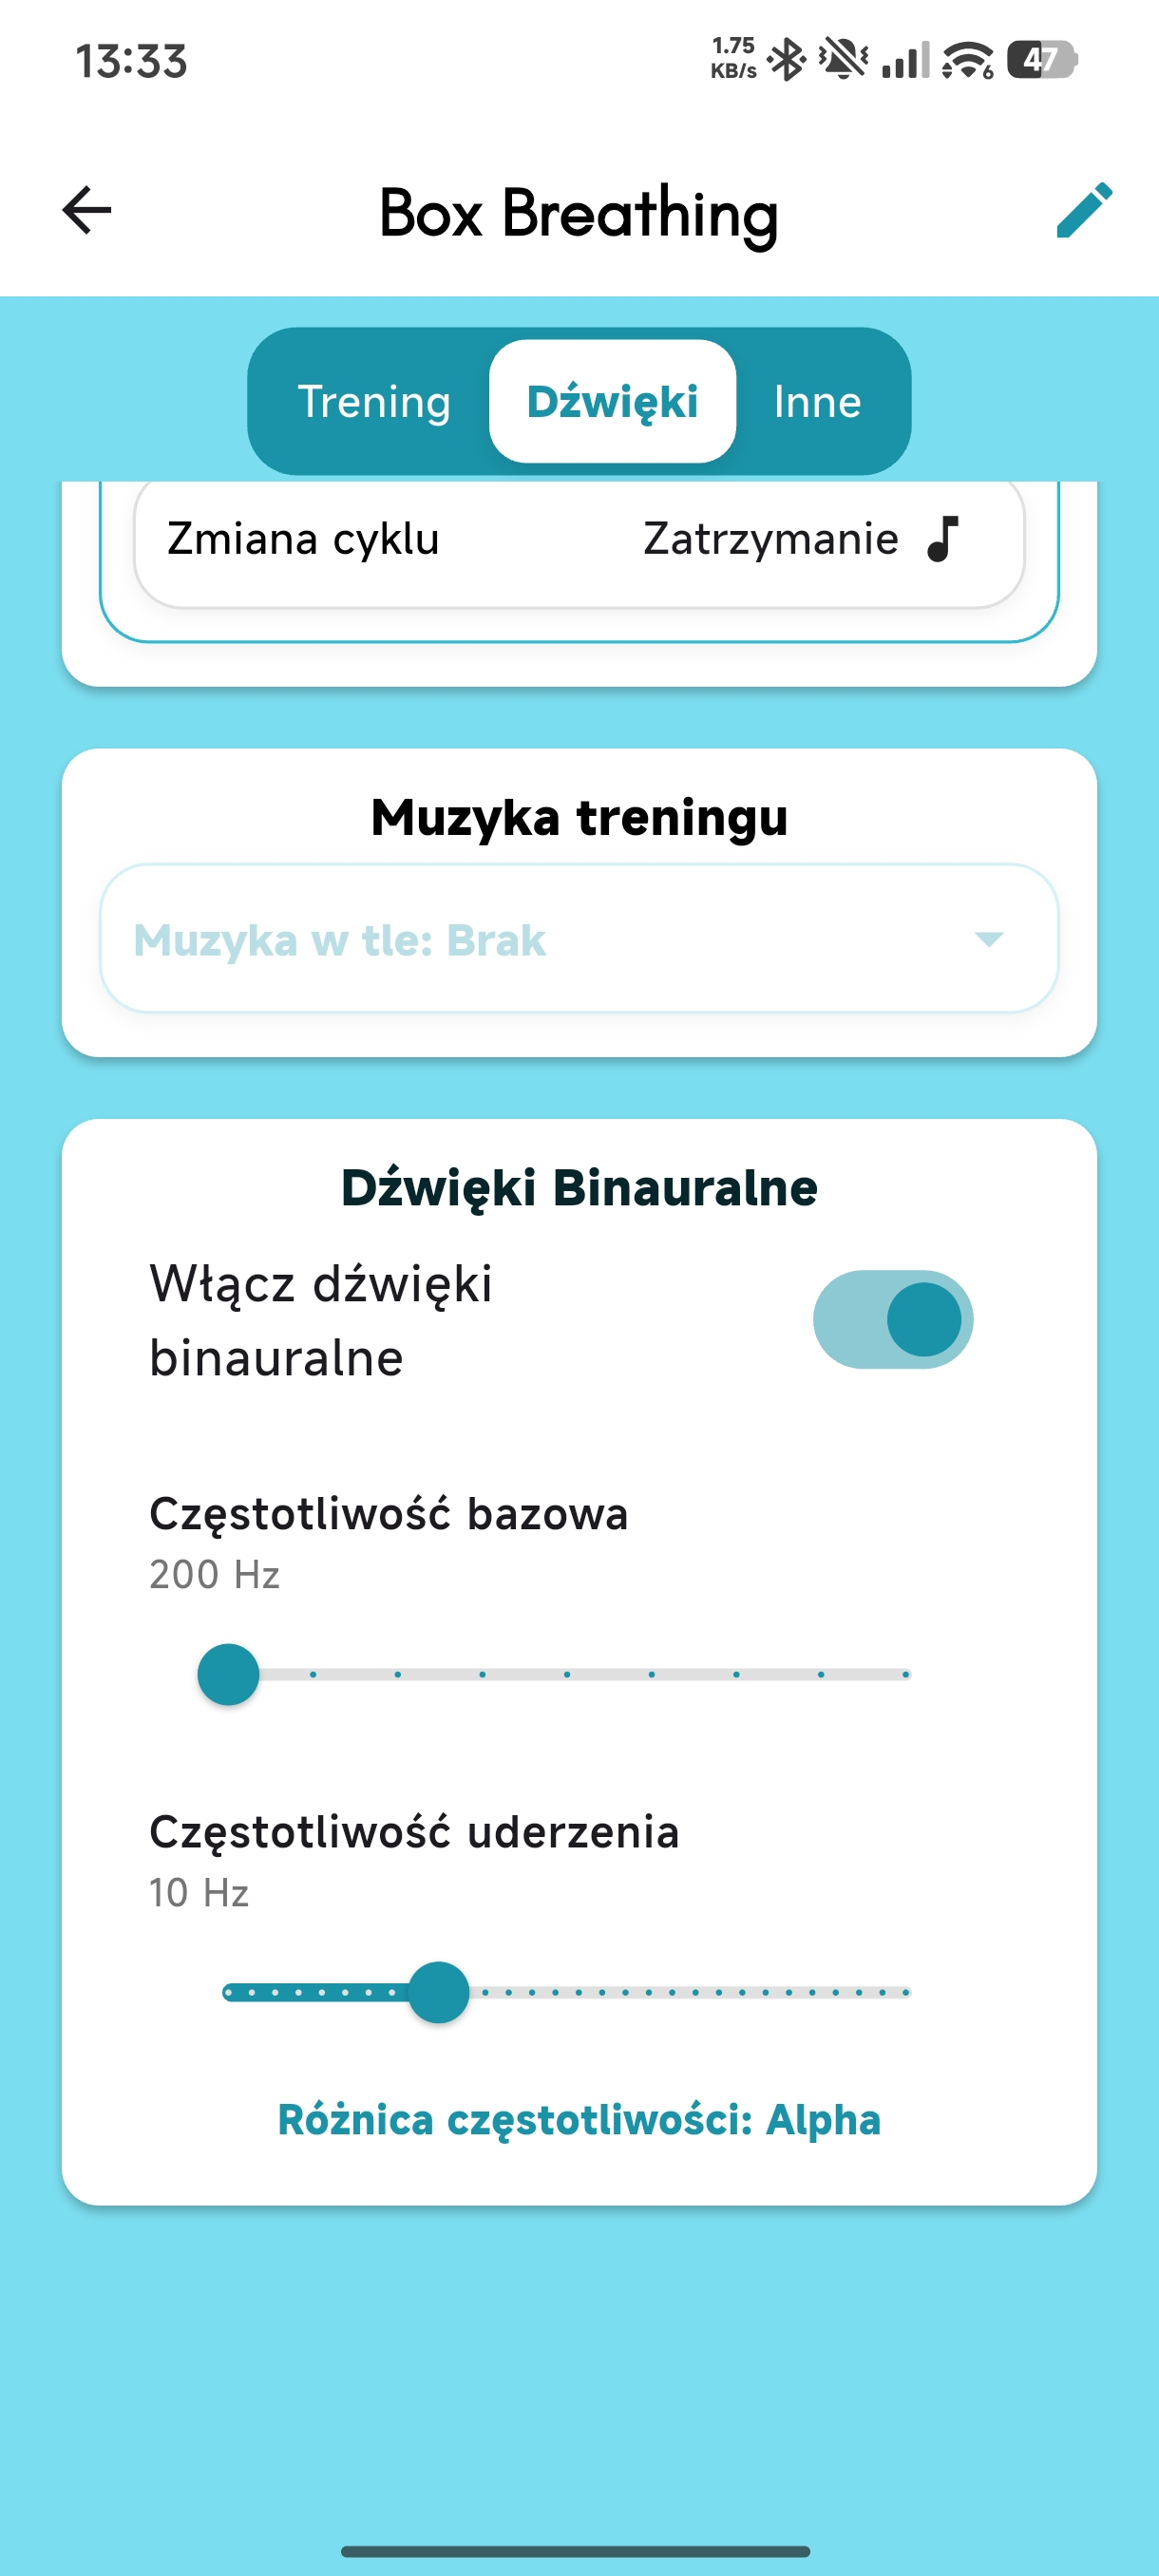
\includegraphics[width=\dimexpr\linewidth-2\fboxrule\relax,height=0.57\textheight,keepaspectratio]{obrazy/badania_interface/sounds_settings_new_binaural.jpg}}}
        \par\small (b)
    \end{minipage}
    \caption[Zmiana sposobu konfiguracji dźwięków binauralnych]{Konfiguracja dźwięków binauralnych: (a) niezależne ustawianie częstotliwości kanałów przed zmianami; (b) wybór częstotliwości bazowej i różnicy częstotliwości po zmianach}
    \label{fig:ux_binaural_settings}
\end{figure}

\subsection{Pozostałe ustawienia treningu}

Zakładkę \textit{Inne} rozszerzono o opcję wygaszania ekranu podczas treningu prowadzonego wyłącznie za pomocą wskazówek dźwiękowych. Użytkownik może określić czas, po którym ekran zostanie wygaszony. Umożliwia to kontynuowanie ćwiczenia bez stałego wyświetlania animacji. W tej samej zakładce umieszczono przełącznik zliczania cykli oddechowych na podstawie sygnału z mikrofonu, dzięki któremu można włączyć lub wyłączyć monitorowanie oddechu.

W dolnej części ekranu dodano wybór stylu wizualizacji opisanego w podrozdziale \ref{sec:ux_breathing_visualization}. Dla widoku osi czasu dostępna jest dodatkowo sonifikacja wskazówek oddechowych. Jej włączenie wyłącza dźwięki binauralne, co zapobiega jednoczesnemu uruchomieniu tych dwóch trybów dźwiękowych. Porównanie zawartości zakładki przed rozbudową i po niej przedstawiono na rysunku \ref{fig:ux_other_settings}.

\begin{figure}[H]
    \centering
    \begin{minipage}[c]{0.44\linewidth}
        \centering
        {\setlength{\fboxsep}{0pt}\setlength{\fboxrule}{0.2pt}\fcolorbox{gray}{white}{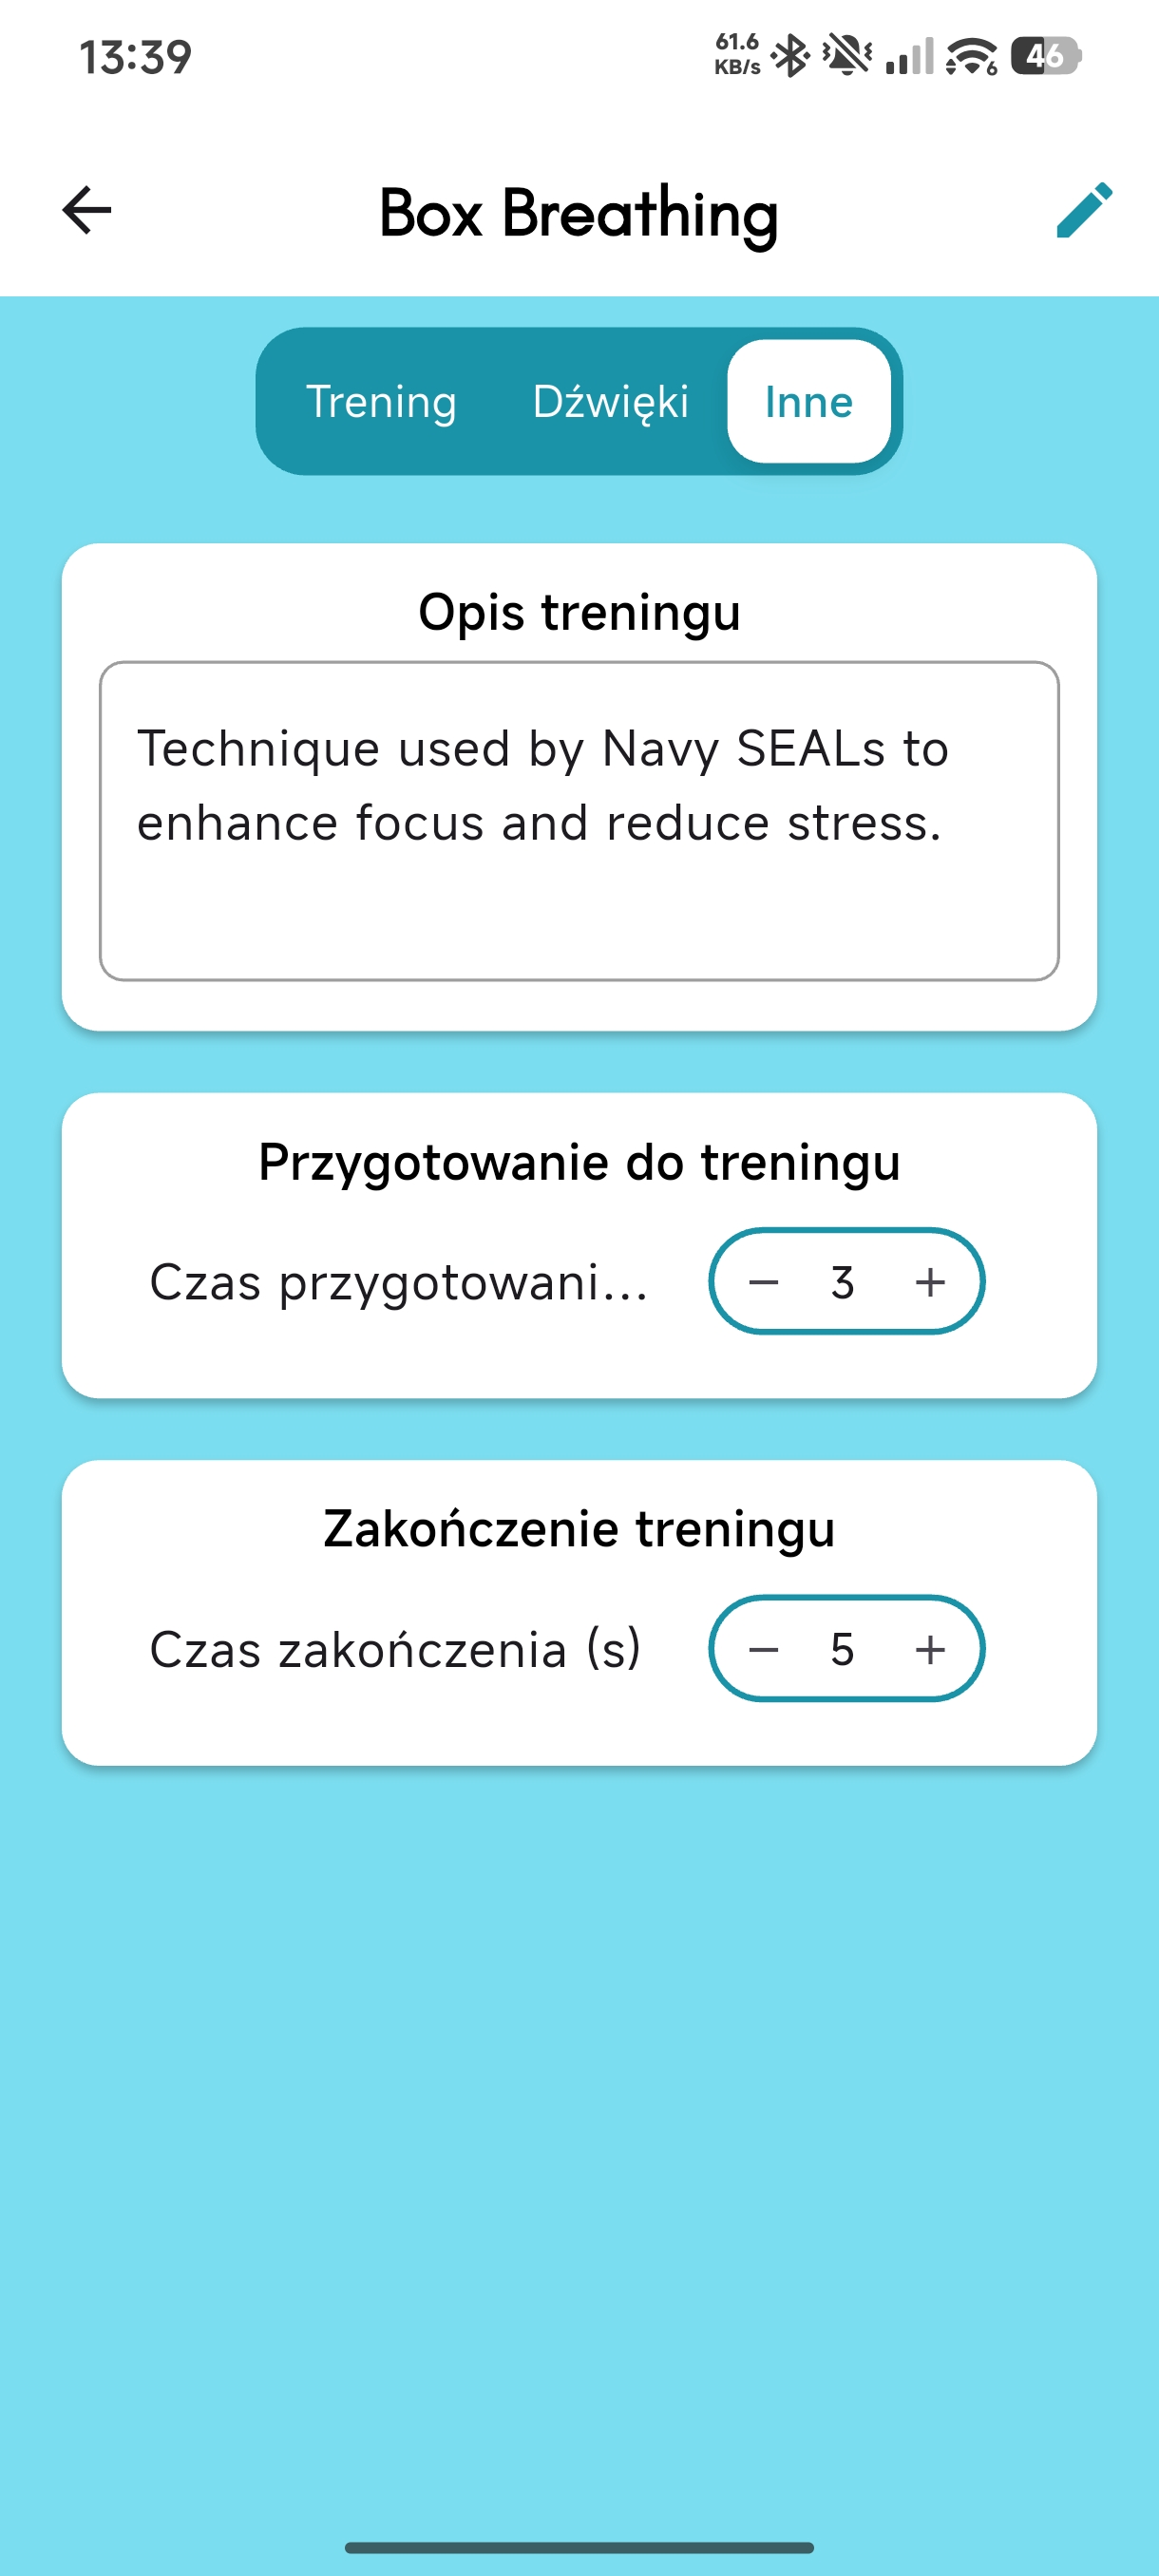
\includegraphics[width=\dimexpr\linewidth-2\fboxrule\relax,height=0.64\textheight,keepaspectratio]{obrazy/badania_interface/other_settings_old.jpg}}}
        \par\small (a)
    \end{minipage}\hfill
    \begin{minipage}[c]{0.08\linewidth}
        \centering
        {\large $\rightarrow$}
    \end{minipage}\hfill
    \begin{minipage}[c]{0.44\linewidth}
        \centering
        {\setlength{\fboxsep}{0pt}\setlength{\fboxrule}{0.2pt}\fcolorbox{gray}{white}{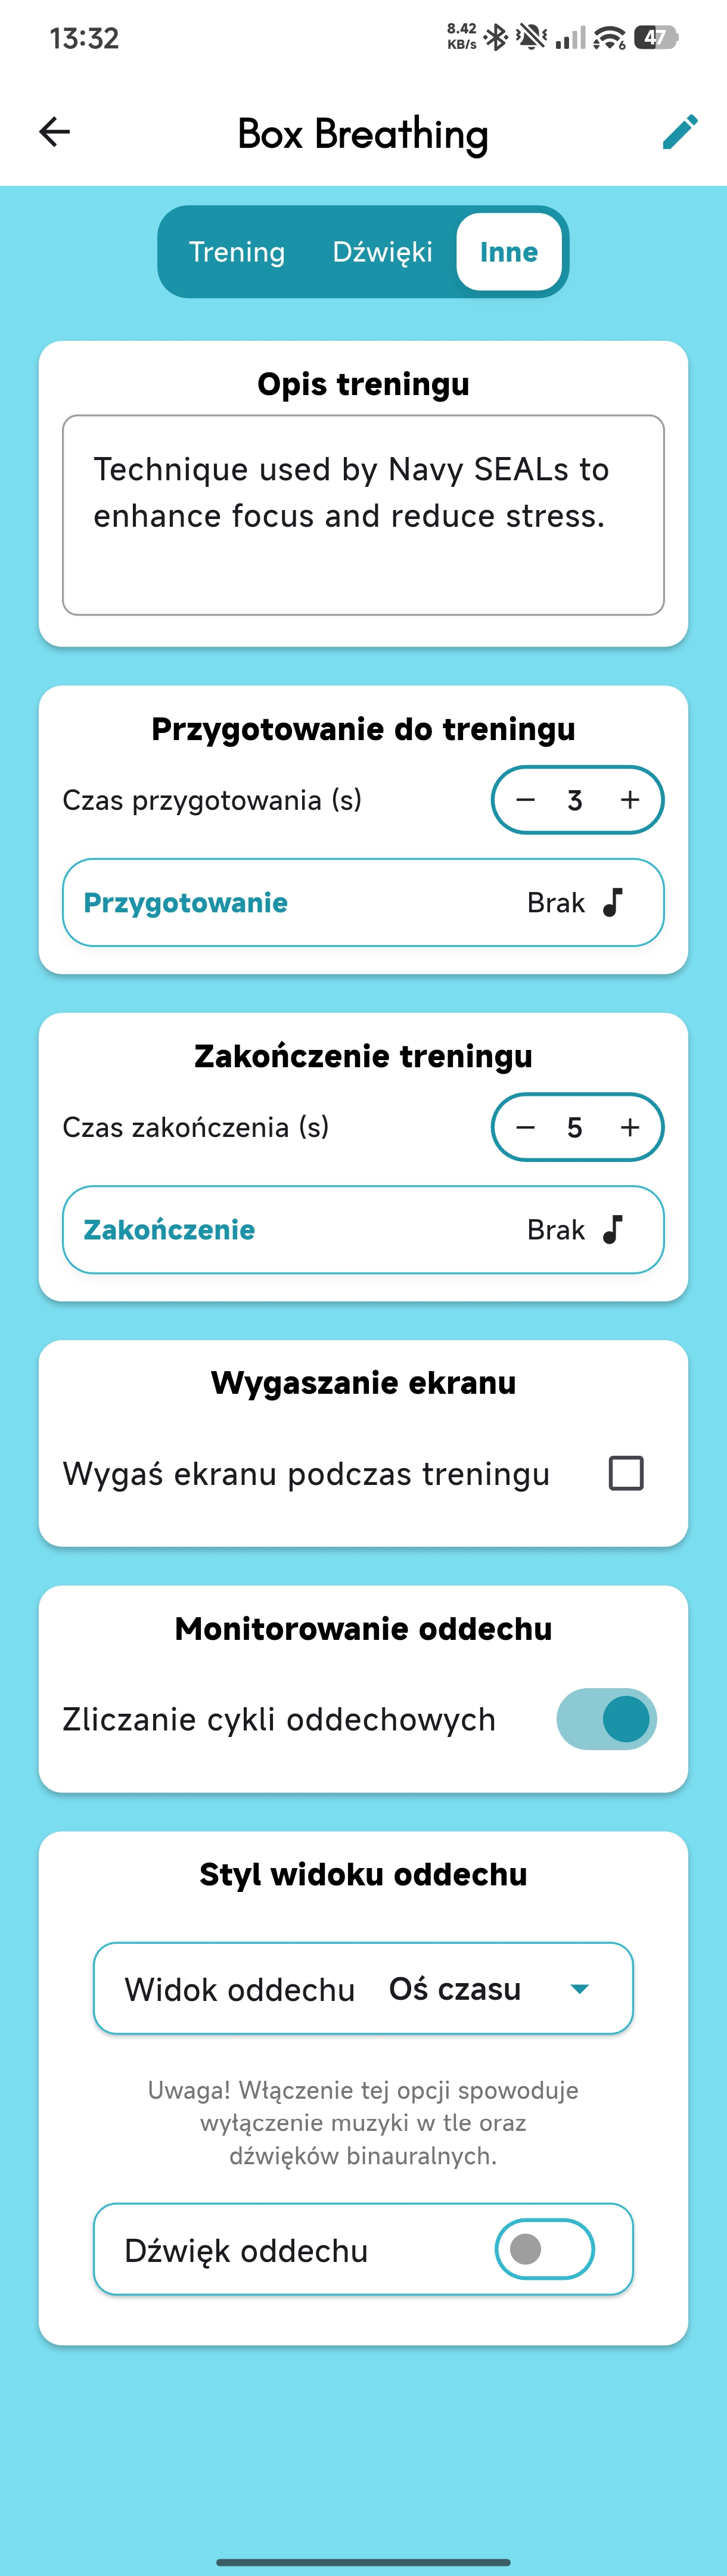
\includegraphics[width=\dimexpr\linewidth-2\fboxrule\relax,height=0.64\textheight,keepaspectratio]{obrazy/badania_interface/other_settings_new.jpg}}}
        \par\small (b)
    \end{minipage}
    \caption[Zakładka Inne przed zmianami i po rozbudowie]{Zakładka Inne: (a) ekran przed zmianami; (b) ekran po dodaniu wygaszania ekranu, monitorowania oddechu i wyboru wizualizacji}
    \label{fig:ux_other_settings}
\end{figure}

\subsection{Kalibracja detekcji wydechu do używanego sprzętu}

Dodano ekran umożliwiający dostosowanie czułości wykrywania wydechu. Użytkownik może zmienić jej wartość za pomocą suwaka, uruchomić test mikrofonu i sprawdzić reakcję detektora na wykonywany wydech. Pozwala to dobrać ustawienie do używanego telefonu oraz zestawu słuchawkowego bez zmiany wag modelu ani ponownego uczenia sieci. Czułość prezentowana w interfejsie nie jest standardowym progiem prawdopodobieństwa klasy \textit{Exhale}: jej zwiększenie ułatwia przypisanie próbki do tej klasy, a więc może zwiększyć zarówno liczbę poprawnych, jak i fałszywych detekcji.

Połączenie regulacji czułości z możliwością bezpośredniego testowania zapewnia informację zwrotną podczas konfiguracji. Użytkownik może sprawdzić, czy wydechy są wykrywane oraz czy detektor reaguje także na inne dźwięki, a następnie skorygować ustawienie. Ekran przedstawiono na rysunku \ref{fig:ux_threshold_tester}. Wyniki doboru czułości w testowanych konfiguracjach sprzętowych omówiono w~dalszej części rozdziału, w podrozdziale dotyczącym testów na urządzeniach mobilnych.

\begin{figure}[H]
    \centering
    {\setlength{\fboxsep}{0pt}\setlength{\fboxrule}{0.2pt}\fcolorbox{gray}{white}{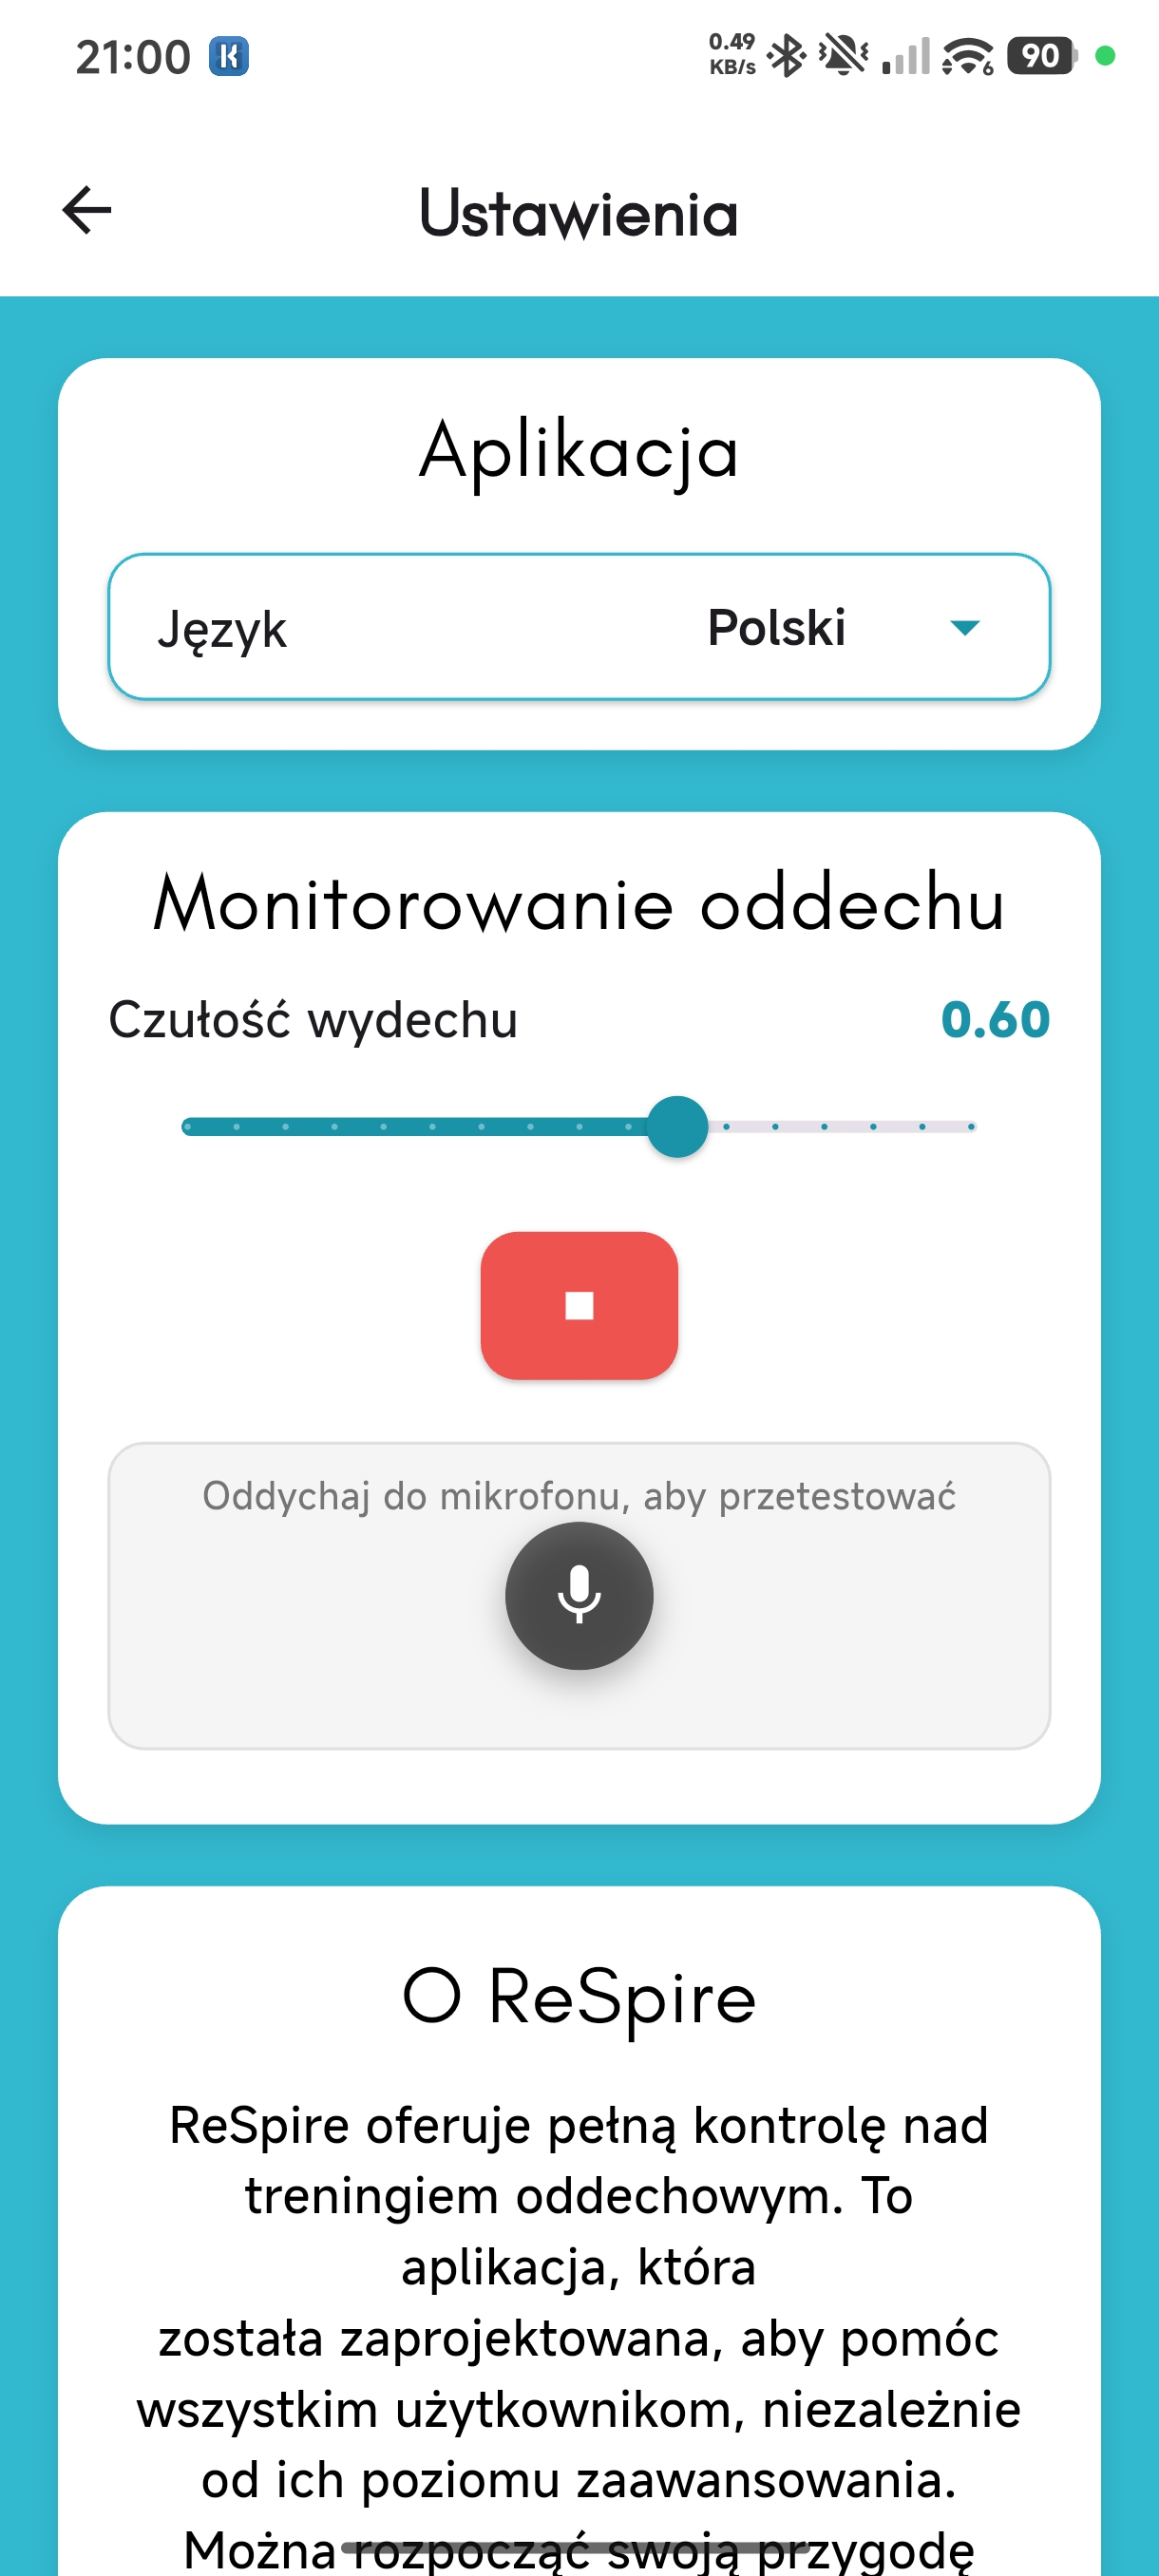
\includegraphics[width=0.43\linewidth,height=0.60\textheight,keepaspectratio]{obrazy/badania_interface/treshold_tester_new.jpg}}}
    \caption{Ekran regulacji czułości i testowania detekcji wydechu z użyciem mikrofonu}
    \label{fig:ux_threshold_tester}
\end{figure}

\section{Usprawnienie działania modelu wykrywania wydechu}

W ramach rozwoju systemu porównano dwie wersje modelu wykrywania wydechu. Model \textit{breathing classification v2} (BCV2) stanowił punkt odniesienia. Udoskonalony model \textit{breathing classification v3} (BCV3) został wytrenowany na rozszerzonym zbiorze danych oraz uzupełniony o mechanizmy ograniczające przeuczenie i wpływ nierównomiernego rozkładu klas. Oba modele oceniono na tym samym zbiorze testowym zawierającym 11~705 próbek dźwięku, w tym 7206 przykładów klasy \textit{Exhale} oraz 4499 przykładów klasy \textit{Other}.

\subsection{Dodatkowe dane}

Podstawowym usprawnieniem BCV3 było zwiększenie liczby danych wykorzystanych podczas uczenia. Większy zbiór zawierał więcej przykładów zróżnicowanych sposobów wykonywania wydechu, a także próbek należących do klasy \textit{Other}. Pozwoliło to modelowi poznać szerszy zakres cech występujących w sygnale i ograniczyć dopasowanie do niewielkiej liczby nagrań. Zwiększenie różnorodności danych jest szczególnie istotne w aplikacji mobilnej, ponieważ natężenie oraz charakter dźwięku oddechu zależą między innymi od użytkownika, odległości od mikrofonu, jak również warunków otoczenia.

\subsection{Dostosowanie architektury}

W architekturze BCV3 dodano warstwy dropout. Podczas treningu losowo wyłączają one część aktywacji, przez co sieć nie może nadmiernie uzależniać predykcji od pojedynczych cech. Rozwiązanie to pełni funkcję regularyzacji i zmniejsza ryzyko przeuczenia, poprawiając zdolność modelu do działania na nagraniach niewykorzystywanych podczas uczenia.

Drugą zmianą było zastosowanie ważonej funkcji straty (ang. \textit{weighted loss}). Klasy w zbiorze treningowym nie były reprezentowane równomiernie, dlatego ich wagi wyznaczono na podstawie udziału poszczególnych klas w danych. Klasa występująca rzadziej otrzymała większą wagę, natomiast częstsza mniejszą. Dzięki temu błąd popełniony dla mniej licznej klasy miał większy wpływ na aktualizację parametrów modelu. Ograniczyło to tendencję sieci do preferowania klasy dominującej oraz pozwoliło uzyskać bardziej zrównoważone wyniki.

\subsection{Porównanie wyników}

Model zwraca dla analizowanego fragmentu dźwięku wartość interpretowaną jako prawdopodobieństwo przynależności do klasy \textit{Exhale}. Próg decyzyjny $\theta$ określa minimalną wartość wymaganą do wykrycia wydechu:

\begin{equation}
    \widehat{y} = \begin{cases}
        \textit{Exhale}, & p(\textit{Exhale}) \geq \theta, \\
        \textit{Other}, & p(\textit{Exhale}) < \theta.
    \end{cases}
\end{equation}

Przykładowo wynik $p(\textit{Exhale})=0{,}62$ zostanie uznany za wydech przy progu 0,5 lub 0,6, ale nie przy progu 0,7. Zwiększenie progu powoduje więc przypisywanie mniejszej liczby próbek do klasy \textit{Exhale}. W konsekwencji maleją wartości TP i FP, natomiast rosną TN i FN.

Badania przeprowadzono dla progów od 0,3 do 0,7. Próg wybierano przez maksymalizację dokładności na zbiorze testowym, zgodnie ze wzorem $\mathrm{Accuracy}=(TP+TN)/(TP+TN+FP+FN)$. Dla BCV3 w formacie ONNX najwyższą wartość uzyskano przy progu 0,5 czyli $89\%$. Nie maksymalizowano osobno czułości ani wyniku F1 klasy \textit{Exhale}. Wybrany został próg zapewniający największy udział wszystkich poprawnych klasyfikacji.

Analiza kilku progów była istotna również ze względu na różnice pomiędzy mikrofonami urządzeń mobilnych. Poszczególne telefony mogą rejestrować dźwięk z inną czułością, poziomem wzmocnienia i charakterystyką szumów, co wpływa na wartości zwracane przez model. Jeden stały próg nie musi zatem zapewniać równie dobrej detekcji na każdym urządzeniu. Z tego względu aplikacja umożliwia regulację odpowiadającej mu czułości bez modyfikowania ani ponownego trenowania modelu.

\begin{table}[htbp]
    \centering
    \caption{Porównanie modeli ONNX dla progu decyzyjnego 0,5}
    \label{tab:model_versions_comparison}
    \scriptsize
    \setlength{\tabcolsep}{4pt}
    \renewcommand{\arraystretch}{1.2}
    \begin{tabular}{@{}lrrrrrr@{}}
        \toprule
        \textbf{Wariant} & \textbf{Dokł.} & \textbf{Prec. E} & \textbf{Czuł. E} & \textbf{F1 E} & \textbf{F1 macro} & \textbf{ROC-AUC} \\
        \midrule
        BCV3 & \textbf{85,89\%} & 84,43\% & \textbf{94,52\%} & \textbf{89,19\%} & \textbf{84,45\%} & 90,19\% \\
        BCV2 & 84,95\% & \textbf{84,80\%} & 92,05\% & 88,28\% & 83,63\% & \textbf{91,56\%} \\
        \bottomrule
    \end{tabular}
\end{table}

BCV3 w formacie ONNX osiągnął dokładność 85,89\%, czyli o 0,94 punktu procentowego więcej od BCV2 przy tym samym progu. Wynik F1 dla klasy \textit{Exhale} wzrósł z 88,28\% do 89,19\%, a jej czułość z 92,05\% do 94,52\%. Wysoka czułość jest istotna z punktu widzenia aplikacji, ponieważ pominięcie wydechu może spowodować niezliczenie wykonanego cyklu oddechowego.

Macierz pomyłek wersji ONNX pokazuje, że przy progu 0,5 BCV3 prawidłowo rozpoznał 6811 z 7206 próbek wydechu, podczas gdy BCV2 rozpoznał ich 6633. Liczba pominiętych wydechów zmniejszyła się z 573 do 395. Jednocześnie liczba próbek klasy \textit{Other} błędnie uznanych za wydech wzrosła z 1189 do 1256. BCV3 przesuwa zatem punkt pracy w stronę większej czułości, co jest korzystne dla zliczania cykli, lecz wymaga uwzględnienia ryzyka dodatkowych fałszywych detekcji.

BCV2 uzyskał nieznacznie wyższy wynik ROC-AUC: 0,9156 w porównaniu z 0,9019 dla BCV3. Oznacza to, że przewaga BCV3 nie występuje dla każdej możliwej wartości progu. Przy przyjętym progu 0,5 BCV3 zapewnia jednak wyższą dokładność, czułość i wynik F1 dla wydechu, dlatego został uznany za lepiej dostosowany do docelowego zastosowania w aplikacji.

\subsection{Macierze pomyłek}

Macierze pomyłek modeli ONNX przeanalizowano dla wszystkich badanych wartości progu. W tabeli \ref{tab:all_confusion_matrices} zastosowano standardowe oznaczenia: TP (ang. \textit{true positive}) oznacza poprawnie wykryty wydech, TN (ang. \textit{true negative}) - poprawnie rozpoznana próbka klasy \textit{Other}, FP (ang. \textit{false positive}) - próbka klasy \textit{Other} błędnie uznany za wydech, natomiast FN (ang. \textit{false negative}) - pominięty wydech.

\begin{table}[htbp]
    \centering
    \caption{Porównanie macierzy pomyłek modeli ONNX dla badanych progów decyzyjnych}
    \label{tab:all_confusion_matrices}
    \scriptsize
    \setlength{\tabcolsep}{4pt}
    \renewcommand{\arraystretch}{1.08}
    \begin{tabular}{@{}lrrrrrr@{}}
        \toprule
        \textbf{Wariant} & \textbf{Próg} & \textbf{TP} & \textbf{TN} & \textbf{FP} & \textbf{FN} & \textbf{Dokł.} \\
        \midrule
        BCV3 & 0,7 & 6214 & \textbf{3599} & 900 & \textbf{992} & 83,84\% \\
        & 0,6 & 6586 & 3402 & 1097 & 620 & 85,33\% \\
        & 0,5 & 6811 & 3243 & 1256 & 395 & \textbf{85,89\%} \\
        & 0,4 & 6932 & 3065 & 1434 & 274 & 85,41\% \\
        & 0,3 & \textbf{7020} & 2837 & \textbf{1662} & 186 & 84,21\% \\
        \midrule
        BCV2 & 0,7 & 6346 & 3535 & 964 & 860 & 84,42\% \\
        & 0,6 & 6502 & 3418 & 1081 & 704 & 84,75\% \\
        & 0,5 & 6633 & 3310 & 1189 & 573 & 84,95\% \\
        & 0,4 & 6755 & 3184 & 1315 & 451 & 84,91\% \\
        & 0,3 & 6871 & 3017 & 1482 & 335 & 84,48\% \\
        \bottomrule
    \end{tabular}
\end{table}

We wszystkich wariantach zwiększanie progu klasy \textit{Exhale} od 0,3 do 0,7 zmniejszało liczbę próbek przypisanych do tej klasy. Dla BCV3 liczba poprawnych detekcji TP spadła z 7020 do 6214, a liczba fałszywych detekcji FP z 1662 do 900. Jednocześnie liczba pominiętych wydechów FN wzrosła ze 186 do 992. Dobór progu stanowi zatem kompromis pomiędzy ograniczaniem fałszywych detekcji a zachowaniem wysokiej czułości wykrywania wydechu.

BCV3 uzyskiwał wyższą dokładność od BCV2 dla progów 0,4, 0,5 i 0,6. Przy skrajnych wartościach 0,3 i 0,7 nieznacznie lepszy był BCV2. Najwyższą dokładność spośród wszystkich konfiguracji, równą 85,89\%, osiągnął BCV3 w formacie ONNX dla progu 0,5. W tym ustawieniu poprawnie wykrył 6811 wydechów, pomijając 395, oraz prawidłowo rozpoznał 3243 próbki klasy \textit{Other}. W porównaniu z BCV2 przy tym samym progu wykrył o 178 wydechów więcej, kosztem 67 dodatkowych fałszywych detekcji.

Najważniejsze macierze dotyczą progu 0,5 i formatu ONNX, ponieważ ten format jest uruchamiany na urządzeniu mobilnym, a wskazany próg zapewnił najwyższą dokładność. Ich bezpośrednie zestawienie przedstawiono na rysunku \ref{fig:model_confusion_matrices}.

\begin{figure}[H]
    \centering
    \begin{minipage}[t]{0.48\linewidth}
        \centering
        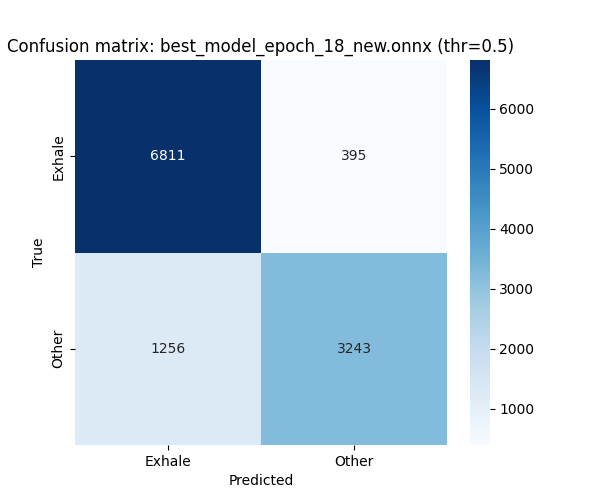
\includegraphics[width=\linewidth]{obrazy/conf_matrix/confusion_best_model_epoch_18_new_onnx_thr_0_5.png}

        \small BCV3
    \end{minipage}
    \hfill
    \begin{minipage}[t]{0.48\linewidth}
        \centering
        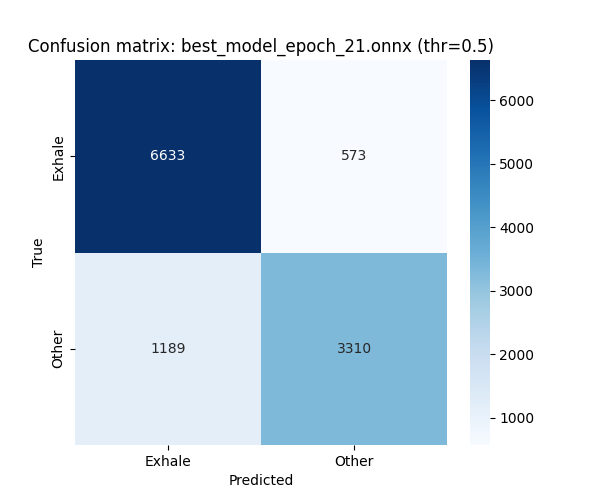
\includegraphics[width=\linewidth]{obrazy/conf_matrix/confusion_best_model_epoch_21_onnx_thr_0_5.png}

        \small BCV2
    \end{minipage}
    \caption{Porównanie macierzy pomyłek modeli BCV3 i BCV2 w formacie ONNX dla progu decyzyjnego 0,5}
    \label{fig:model_confusion_matrices}
\end{figure}

\subsection{Testy na urządzeniach mobilnych}
\subsubsection{Dostosowanie czułości detekcji}
Działanie modelu BCV3 sprawdzono również w warunkach zbliżonych do docelowego wykorzystania aplikacji. Testy przeprowadzono z użyciem emulatora Pixel 3a oraz fizycznych urządzeń Xiaomi Redmi Note 14 Pro i Huawei Mate 20 Lite. Poszczególne konfiguracje różniły się zastosowanym zestawem słuchawkowym, sposobem jego podłączenia oraz dobraną wartością czułości. Zestawienie wykorzystanych konfiguracji przedstawiono w tabeli \ref{tab:mobile_device_thresholds}.

\begin{table}[htbp]
    \centering
    \caption{Konfiguracje wykorzystane podczas testowania modelu na urządzeniach mobilnych}
    \label{tab:mobile_device_thresholds}
    \small
    \setlength{\tabcolsep}{5pt}
    \renewcommand{\arraystretch}{1.2}
    \begin{tabularx}{\textwidth}{@{}p{3.4cm}X p{2.7cm}p{2.1cm}@{}}
        \toprule
        \textbf{Urządzenie} & \textbf{Zestaw słuchawkowy} & \textbf{Połączenie} & \textbf{Dobrana czułość} \\
        \midrule
        Emulator (Pixel 3a) & HyperX Cloud Alpha & Mini jack 3{,}5mm & 0,6 \\
        \midrule
        Huawei Mate 20 Lite & HyperX Cloud Alpha & Mini jack 3{,}5mm & 0,6 \\
        \midrule
        Redmi Note 14 Pro & Poly Blackwire 3220 & USB-C & 0,7 \\
        \bottomrule
    \end{tabularx}
\end{table}

W przypadku emulatora Pixel 3a czułość ustawiono na 0,6 przy wykorzystaniu mikrofonu zestawu HyperX Cloud Alpha. Ten sam zestaw i wartość zastosowano podczas testów na urządzeniu Huawei Mate 20 Lite, gdzie słuchawki podłączono przez złącze mini jack. Dla telefonu Xiaomi Redmi Note 14 Pro użyto zestawu Poly Blackwire 3220 podłączonego przez USB-C, a czułość zwiększono do 0,7. W standardowej interpretacji odpowiada to progom klasy \textit{Exhale} równym odpowiednio 0,4 i 0,3.

Wartości dla urządzeń mobilnych dobrano empirycznie za pomocą ekranu testowania mikrofonu. Przed rozpoczęciem właściwego testu użytkownicy samodzielnie wybierali ustawienie czułości, które w ich subiektywnym odczuciu zapewniało najlepsze działanie detekcji. Sprawdzali przy tym, czy wykonywane wydechy są wykrywane oraz czy inne dźwięki nie powodują nadmiarowych wskazań. Nie maksymalizowano w tym przypadku formalnej miary na oznaczonym zbiorze mobilnym, dlatego wartości te określono jako dobraną czułość, a nie matematycznie optymalny próg. Konieczność zastosowania różnych ustawień potwierdza wpływ charakterystyki mikrofonu, sposobu podłączenia oraz toru przetwarzania dźwięku w urządzeniu.

\subsubsection{Testy wykrywania wydechu podczas treningu}

Skuteczność wykrywania wydechu sprawdzono dodatkowo podczas wykonywania ćwiczeń oddechowych przez użytkowników. Badanie przeprowadzono z użyciem zestawów HyperX Cloud Alpha i Poly Blackwire 3220, zarówno w cichym, jak i głośnym otoczeniu. Każdy uczestnik wykonywał cztery rodzaje treningu: sekwencję obejmującą 4~s wdechu, 2~s wstrzymania oddechu oraz 4~s wydechu, a także symetryczne sekwencje wdechu i wydechu trwające odpowiednio 2~s, 1,5~s oraz 1~s. Dla każdej konfiguracji wartością referencyjną było 30 rzeczywistych wydechów. W tabeli \ref{tab:headset_detection_ratio} przedstawiono zagregowane wyniki pięciu uczestników i obu warunków otoczenia.

Do oceny zastosowano współczynnik detekcji DR (ang. \textit{Detection Ratio}), obliczany według wzoru:

\begin{equation}
    \mathrm{DR} = \frac{N_{\mathrm{det}}}{N_{\mathrm{ref}}} \cdot 100\%,
\end{equation}

gdzie $N_{\mathrm{det}}$ oznacza liczbę wykrytych wydechów, a $N_{\mathrm{ref}}$ liczbę rzeczywistych wydechów.

Wartość DR równa 100\% oznacza zgodność liczby detekcji z liczbą rzeczywistych wydechów. Wynik poniżej 100\% wskazuje na pomijanie wydechów, natomiast wynik przekraczający 100\% oznacza występowanie dodatkowych, fałszywych detekcji. Współczynnik ten opisuje zgodność liczby wykryć, ale nie rozstrzyga, czy każda detekcja została czasowo przypisana do właściwego wydechu.

\begin{table}[H]
    \centering
    \caption{Wyniki wykrywania wydechu dla zestawów HyperX Cloud Alpha i Poly Blackwire 3220}
    \label{tab:headset_detection_ratio}
    \small
    \setlength{\tabcolsep}{5pt}
    \renewcommand{\arraystretch}{1.2}
    \begin{tabular}{@{}lrrrr@{}}
        \toprule
        & \multicolumn{2}{c}{\textbf{HyperX}} & \multicolumn{2}{c}{\textbf{Blackwire}} \\
        \midrule
        \textbf{Test} & \textbf{Detekcje} & \textbf{DR} & \textbf{Detekcje} & \textbf{DR} \\
        \midrule
        4-2-4       & 28,7/30 & 95,60\% & 35,5/30 & 118,30\% \\
        2~s           & 29,0/30 & 96,70\% & 28,0/30 & 93,30\% \\
        1,5~s         & 21,0/30 & 70,00\% & 22,0/30 & 73,30\% \\
        1~s           & 5,0/30  & 16,70\% & 6,0/30  & 20,00\% \\
        \bottomrule
    \end{tabular}
\end{table}

Najlepsze wyniki dla zestawu HyperX uzyskano dla wolniejszych sekwencji 4-2-4 oraz 2~s, dla których DR wyniósł odpowiednio 95,60\% i 96,70\%. Zestaw Blackwire osiągnął zbliżony rezultat dla sekwencji 2~s, natomiast w teście 4-2-4 wartość 118,30\% wskazuje na nadmiarowe detekcje. Wraz ze skracaniem faz skuteczność obu konfiguracji wyraźnie malała. Dla sekwencji 1,5~s współczynnik DR osiągnął 70,00\% dla HyperX i 73,30\% dla Blackwire, a dla najszybszej sekwencji 1~s jedynie 16,70\% oraz 20,00\%.

Wyniki wskazują, że obecna wersja modelu lepiej współpracuje z wolniejszymi treningami, w których dźwięk wydechu trwa wystarczająco długo, aby został prawidłowo zarejestrowany i~sklasyfikowany. Krótkie fazy stanowią większe wyzwanie ze względu na ograniczoną liczbę analizowanych fragmentów sygnału oraz niewielkie odstępy między kolejnymi oddechami. Różnice pomiędzy zestawami potwierdzają również znaczenie charakterystyki mikrofonu, a także dobranej czułości detekcji.

\chapter{Dyskusja}

Praca obejmowała rozwój aplikacji ReSpire oraz modelu wykrywania wydechu, a następnie połączenie obu elementów w system wspomagający trening oddechowy. Uzyskane rozwiązanie umożliwia personalizację ćwiczeń, prowadzenie sesji za pomocą wskazówek wizualnych lub dźwiękowych oraz zliczanie cykli na podstawie sygnału z mikrofonu. W niniejszym rozdziale odniesiono osiągnięte rezultaty do założonych celów, wskazano ograniczenia obecnej wersji i~przedstawiono kierunki dalszego rozwoju.

\section{Realizacja założonych celów}

Założony cel osiągnięto w zakresie stworzenia narzędzia łączącego personalizację treningu z podstawowym monitorowaniem jego przebiegu. Najważniejszym rezultatem nie jest jednak pojedyncza funkcja, lecz połączenie części aplikacyjnej oraz badawczej w rozwiązanie, które można sprawdzać podczas rzeczywistego ćwiczenia. Rozwój wcześniejszych projektów pozwolił skupić się na ich wzajemnym uzupełnieniu oraz dostosowaniu do wspólnego zastosowania.

Aplikacja daje użytkownikowi swobodę definiowania ćwiczeń, natomiast możliwość sprawdzania ich wykonania pozostaje bardziej ograniczona. Jest to istotne rozróżnienie między gotowością narzędzia do prowadzenia treningu a dojrzałością jego funkcji monitorujących.

\section{Interpretacja wyników i ograniczenia}

Aplikacja ReSpire zapewnia pełny zestaw funkcji potrzebnych do konfigurowania i prowadzenia treningów oddechowych. Włączenie modelu BCV3 wzbogaca ją o możliwość automatycznego zliczania cykli, nadając projektowi również wymiar badawczy. Pozwala to sprawdzać, w jakim stopniu analiza dźwięku może uzupełniać prowadzenie ćwiczeń o informację zwrotną na temat ich przebiegu.

Wyniki testów przeprowadzonych z udziałem użytkowników wskazują, że przydatność detekcji zależy przede wszystkim od tempa ćwiczenia. Dla wolniejszych wzorców liczba wykrytych wydechów była zbliżona do wartości referencyjnej, co potwierdza możliwość wykorzystania modelu do wspomagania typowych treningów oddechowych. Wyraźny spadek współczynnika DR dla faz trwających 1,5~s i 1~s pokazuje jednak, że obecne rozwiązanie nie reaguje dostatecznie niezawodnie podczas szybkich sekwencji. Krótki wydech może obejmować zbyt mało analizowanych fragmentów sygnału, a niewielki odstęp pomiędzy kolejnymi fazami dodatkowo utrudnia ich rozdzielenie.

Różnice pomiędzy zestawami HyperX i Blackwire potwierdzają wpływ toru rejestracji dźwięku na działanie modelu. Wartość DR przekraczająca 100\% dla zestawu Blackwire w teście 4-2-4 oznacza, że zwiększenie czułości nie zawsze prowadzi do dokładniejszego zliczania, ponieważ może powodować wielokrotne lub fałszywe detekcje.

Obecna wersja detekcji ma charakter eksperymentalny oraz stanowi demonstrację wykonalności koncepcji (ang. \textit{proof of concept}). Uzyskane wyniki wskazują, że model może skutecznie wspomagać zliczanie cykli podczas treningów wykorzystujących wolniejsze fazy oddechu. W przypadku szybszych sekwencji jego skuteczność jest jednak niewystarczająca, dlatego zastosowanie modelu w takich treningach wymaga dalszego usprawnienia sposobu detekcji.

\section{Kierunki dalszego rozwoju}

Istotnym kierunkiem dalszych prac jest uzupełnienie obsługi systemu iOS. Warstwa aplikacyjna została przygotowana do pracy na urządzeniach z tym systemem, jednak natywna integracja modelu BCV3 w kodzie Swift nie została przeprowadzona. Gotowości wspólnej warstwy aplikacji nie należy więc utożsamiać z pełnym działaniem detekcji wydechu na iOS. Dokończenie tego etapu wymaga przygotowania obsługi modelu w warstwie natywnej, połączenia jej z~kodem Flutter oraz sprawdzenia całego procesu na fizycznych urządzeniach. Testy powinny objąć zgodność przetwarzania sygnału, poprawność predykcji, a także działanie aplikacji podczas sesji treningowej.

Drugim kierunkiem jest dalsze usprawnianie modelu BCV3. Warto rozszerzać zbiór danych o nagrania większej liczby użytkowników, różnych mikrofonów i warunków otoczenia, w tym dźwięków mogących powodować fałszywe detekcje. Kolejne eksperymenty mogą dotyczyć architektury sieci, sposobu przygotowania sygnału oraz parametrów uczenia. Poszczególne modyfikacje powinny być oceniane oddzielnie, aby ustalić ich rzeczywisty wpływ na wynik. Celem powinno być nie tylko zwiększanie czułości, lecz także ograniczanie błędnego zliczania cykli.

W przyszłości model można również rozbudować o wykrywanie wszystkich faz oddechu. Pozwoliłoby to pełniej monitorować przebieg ćwiczenia, jak również odnosić go do zaplanowanego wzorca. Aby takie rozwiązanie działało niezawodnie, konieczne będzie jednak zwiększenie skuteczności rozpoznawania poszczególnych faz. Rozszerzenie zakresu detekcji powinno zatem iść w parze z~poprawą jakości predykcji, tak aby przekazywana użytkownikowi informacja zwrotna była wiarygodna.

\section{Wnioski końcowe}

Rezultatem pracy jest funkcjonalnie kompletna aplikacja do personalizacji i prowadzenia treningów oddechowych, rozszerzona o eksperymentalny moduł wykrywania wydechu. Zrealizowana na Androidzie integracja BCV3 stanowi podstawę dalszych badań nad automatycznym monitorowaniem ćwiczeń. Dalsze prace mogą koncentrować się na poprawie skuteczności tego dodatku oraz jego natywnej integracji na iOS, przy zachowaniu niezależności podstawowych funkcji treningowych od modelu detekcji.
% ---------------------- Bibliografia -----------------------
\nocite{*} % dodajemy całą zawartość refs.bib
\printbibliography[heading=bibintoc,title={Bibliografia}]
% -----------------------------------------------------------

%------------------------------------------------------------
%	Dodanie wykazu rysunków oraz tabeli

\renewcommand{\baselinestretch}{1.0}\normalsize	% interlinia w sekcji wykazów
\addcontentsline{toc}{chapter}{\listfigurename}	% dodanie wykazu rysunków do spisu treści
\listoffigures									% generacja wykazu rysunków

\addcontentsline{toc}{chapter}{\listtablename}	% dodanie wykazu tabel do spisu treści
\listoftables									% generacja wykazu tabel
\renewcommand{\baselinestretch}{1.3}\normalsize	% powrót do interlinii 1.5


% ---------------------- DODATKI -----------------------\
\appendix
%\addcontentsline{toc}{chapter}{Dodatek A}
% Zależnie od dodatku, zaleca się dodawnie dodatków jako
% dokumenty PDF
% \includepdf{dodatki/dodatek1.pdf}
%\include{dodatki/instrukcja_uzytkowania}
%\include{dodatki/repozytorium}

% -----------------------------------------------------------
\end{document}
%------------------------------------------------------------
			 	%	Koniec pracy dyplomowej  %
%------------------------------------------------------------
